\section[Offline/Postmortem Analysis]{Offline Analysis}
\label{sec:offline}

Power grid studies on distribution of frequency deviation/fluctuation aid in developing suitable control mechanisms for power grid operators. Conventionally, the Gaussian model has been used to model its distribution \cite{woodAndWollenbergPowerGenerationOperationAndControl}, but certain features of real power grids such as heavier tails (i.e. when the PDF of frequency fluctuations at a distance of several standard deviation have a significantly higher magnitude than the corresponding PDF magnitudes of the assumed Gaussian distribution. This is also called as having a high kurtosis), skewness (frequency fluctuations being asymmetric around the mean) and even having bimodal or multimodal distributions are not explained by the simple model. The first part of the `Offline Analysis' chapter explores this aspect by plotting PDFs of several world power grid frequency archives and visually analyzing the results.
 
Various frequency time-series archives for a diverse set of real-world grids were obtained and analyzed by plotting their bulk distribution probability density functions and autocorrelation decay functions. The data for most European and US grids was conveniently curated by the authors of \cite{lrydin01, lrydinGithub}. For the other regions of the world, \cite{tokyo2017, tokyo2020} had the data for the Tokyo grid, \cite{nordic2018, nordic2019} for the Nordic grids, \cite{ce2019, ce2020} for Continental European grid and \cite{ukNationalGridESOData} for the UK Grid.
All time series were collected at sampling rates between 0.5 seconds (Tokyo) and 10 seconds (Continental Europe). Refer to Table \ref{tab:realGridSamplingData} for further details on sampling times and total duration of sampling.

\renewcommand{\arraystretch}{1.0}

\begin{table}[!ht]
	\centering
	\caption{Grid-wise sampling data}
	\label{tab:realGridSamplingData}
	\begin{tabular}{c|c|c|c|c}
		\toprule
		Grid & 
		\begin{tabular}{c}
			Nominal\\
			Frequency\\
		\end{tabular} & 
		\begin{tabular}{c}
			Sampling \\
			time\\
		\end{tabular} & 
		\begin{tabular}{c}
			Total\\
			Sampled\\
			Duration\\
		\end{tabular} & 
		\begin{tabular}{c}
			Presented\\
			in Fixed Time\\
			Autocorrelation Plot?\\
		\end{tabular}\\
		\midrule
		\begin{tabular}{c}
			Continental \\
			European (CE) \\
		\end{tabular}
		& $50$Hz & $1$s &  \begin{tabular}{c}
			$1$ year\\
			(2019)\\
		\end{tabular} & Yes \\[15pt]
		Nordic & $50$Hz & $0.5$s & \begin{tabular}{c}
			$2$ years\\
			(2018 and 2019)\\
		\end{tabular} & Yes \\[15pt]
		\begin{tabular}{c}
			Great\\
			Britain (GB)
		\end{tabular} & $50$Hz & $0.5$s & \begin{tabular}{c}
			$2$ years\\
			(2019 and 2020)\\
		\end{tabular} & Yes\\[15pt]
		\begin{tabular}{c}
			Mallorcan \\
			(Spain) \\
		\end{tabular} & $50$Hz &  $1$s & \begin{tabular}{c}
			$3$ months\\
			(Oct to Dec 2019)\\
		\end{tabular} & Yes\\[15pt]
		\begin{tabular}{c}
			Western\\
			Interconnection \\
			(US-WI)\\
		\end{tabular} & $60$Hz & $1$s & \begin{tabular}{c}
			$7$ days\\
			(in May 2019)\\
		\end{tabular} & Yes\\[25pt]
		\begin{tabular}{c}
			Texas\\
			(US-TX)\\
		\end{tabular} & $60$Hz & $1$s & \begin{tabular}{c}
			$3$ days\\
			(in May 2019)\\
		\end{tabular} & No\\[15pt]
		Tokyo & $50$Hz & $1$s & \begin{tabular}{c}
			$5$ months\\
			(Jan, July, Aug,\\
			Oct, Dec 2020)\\
		\end{tabular} & No\\[25pt]
		\begin{tabular}{c}
			France\\
			(RTE)
		\end{tabular} & $50$Hz & $10$s & \begin{tabular}{c}
			$1$ year\\
			(2019)\\
		\end{tabular} & No\\[15pt]
		\begin{tabular}{c}
			Indian\\
			(NRLDC)
		\end{tabular} & $50$Hz & $30$s & \begin{tabular}{c}
			$5$ days\\
			($3$ days in 2019\\
			and $2$ days in 2020)\\
		\end{tabular} & No\\[25pt] 
		\bottomrule
	\end{tabular}
\end{table}


For all grids, the frequency data was:
\begin{itemize}
	\item plotted as a Probability Distribution Function (PDF)
	\item used to estimate values for mean $\mu$ and standard deviation $\sigma$ in order to plot the closest fitting Gaussian curve denoted by
	\begin{equation}
		PDF(f) = \frac{1}{\sigma \sqrt{2\pi}}\exp{\left\{-\frac{1}{2}\left(\frac{f-\mu}{\sigma^2}\right)\right\}}
	\end{equation}
\end{itemize}
with the objective of visually checking the level of agreement/disagreement between the generally used Gaussian curve used to model grid frequency PDFs.

\begin{figure}[!ht]
	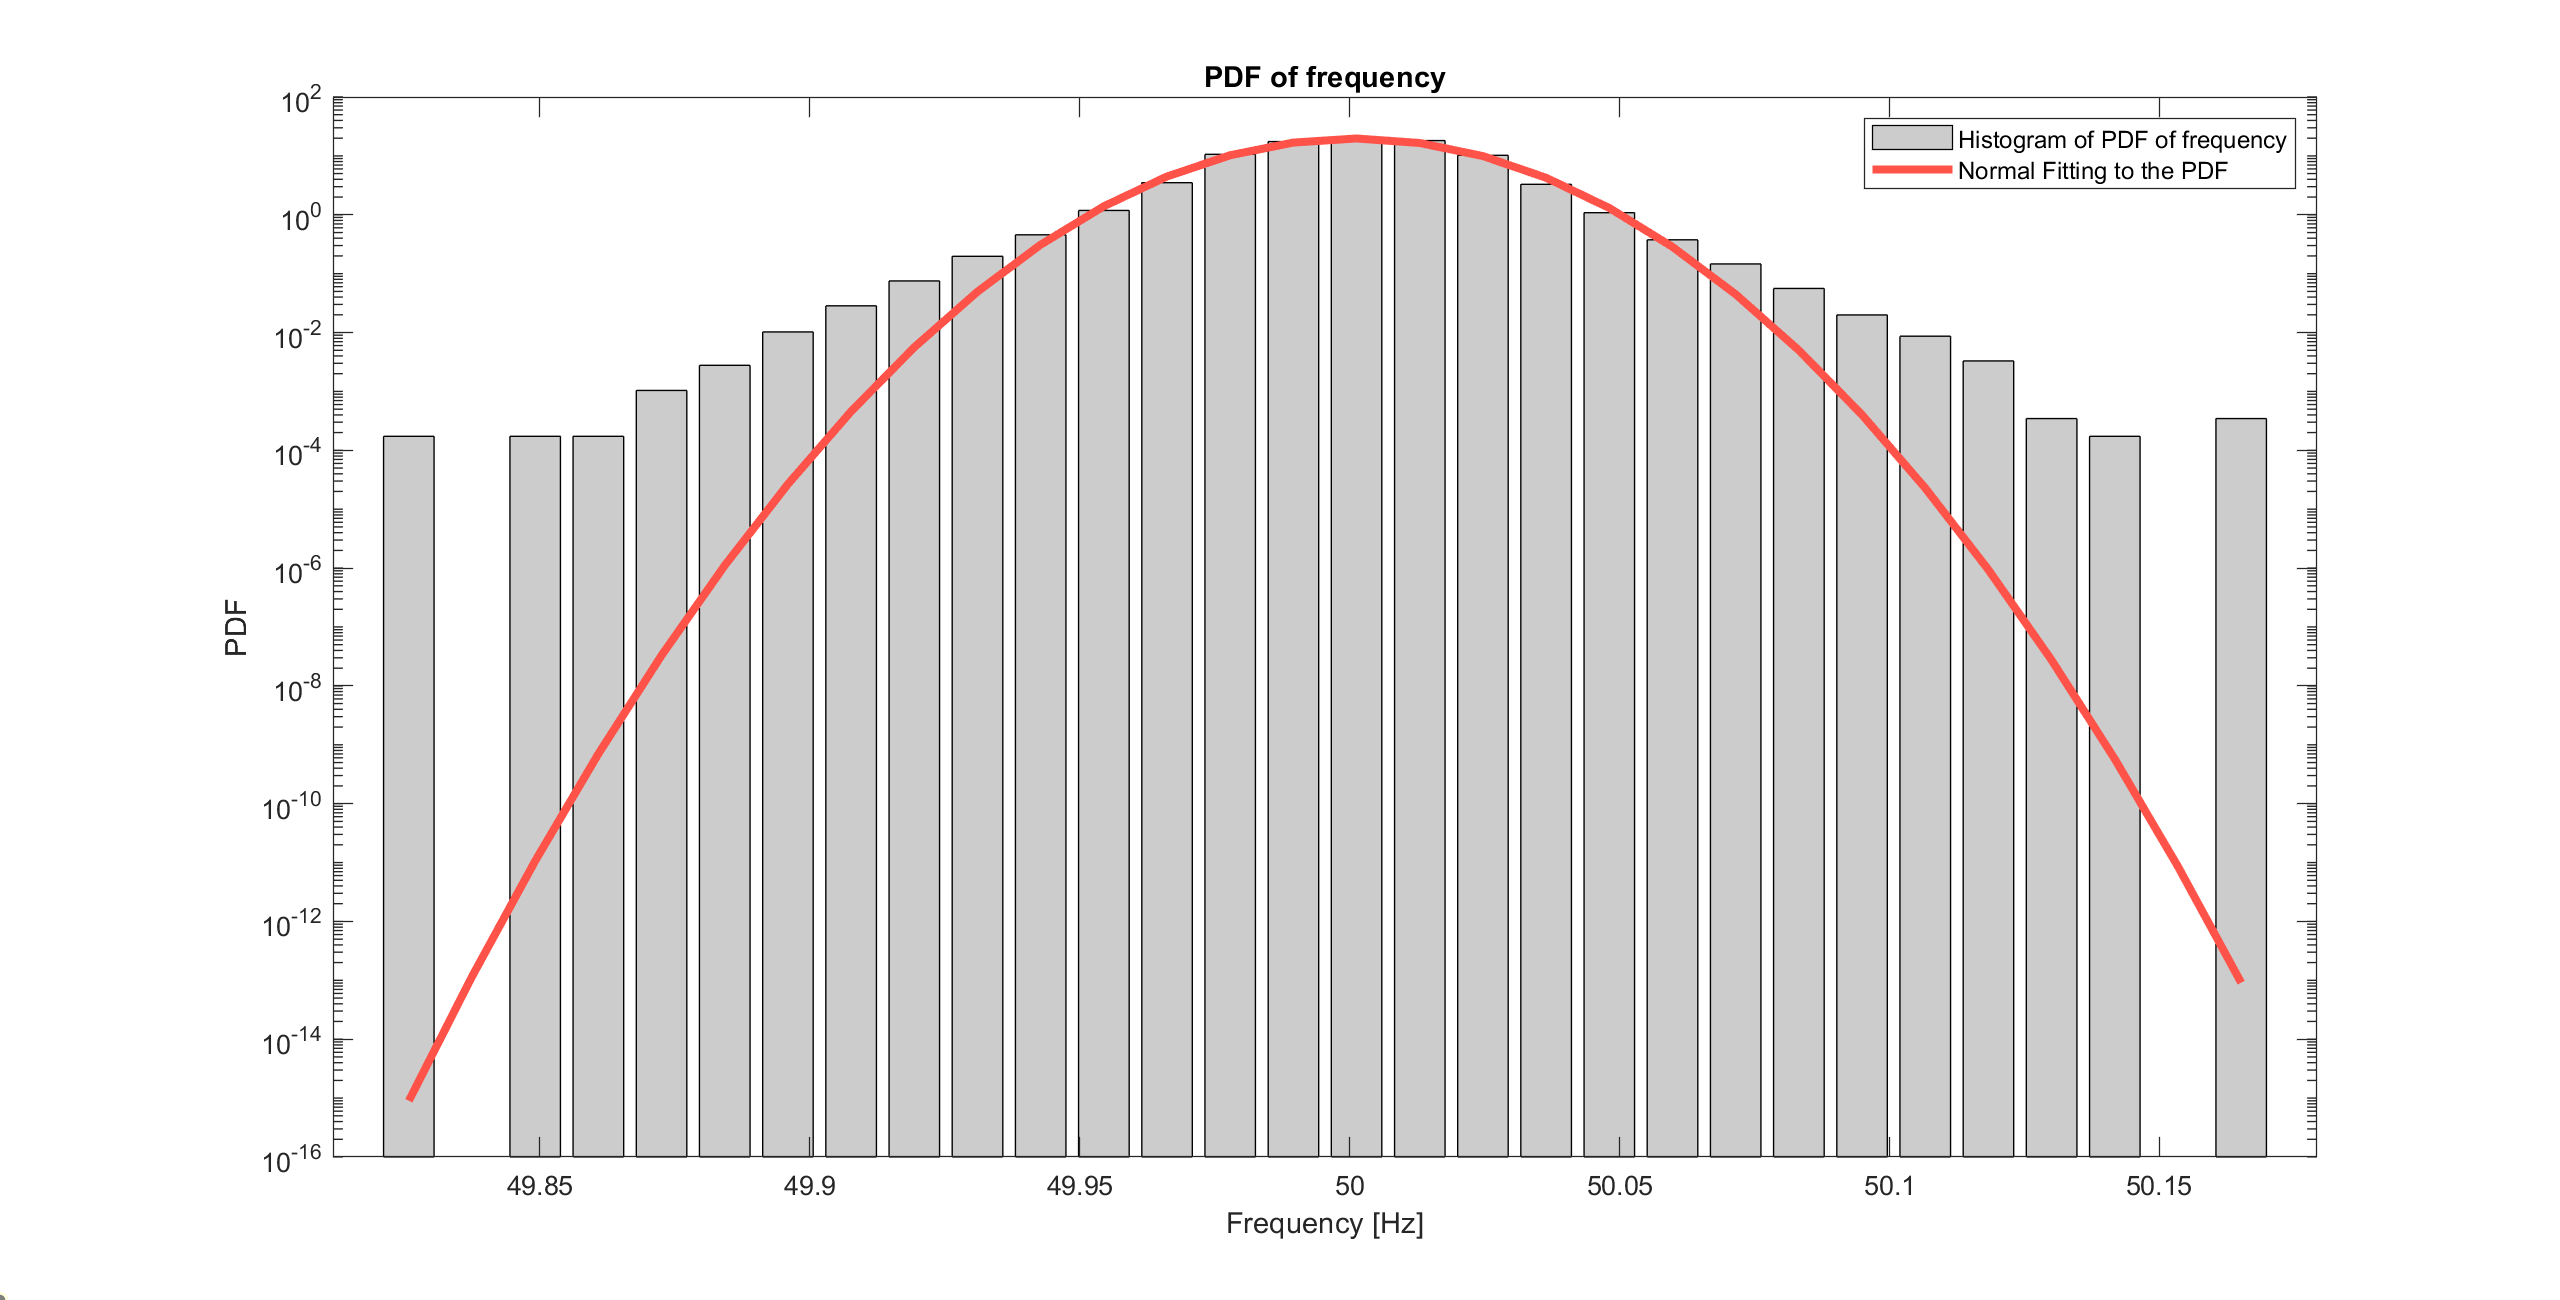
\includegraphics[scale=0.25]{../figures/pdf/pdf_frequency_continental_europe_2019}
	\caption{Frequency Probability Density Function plots for the Continental European grid for the year 2019. There is significant deviation of the actual PDF values (grey bars) from the closest Gaussian model fitted to the same data (red curve) at the tails, which are much heavier in the former.	}
\end{figure}

\begin{figure}[!ht]
	\centering
	\begin{subfigure}{\textwidth}
		\centering
		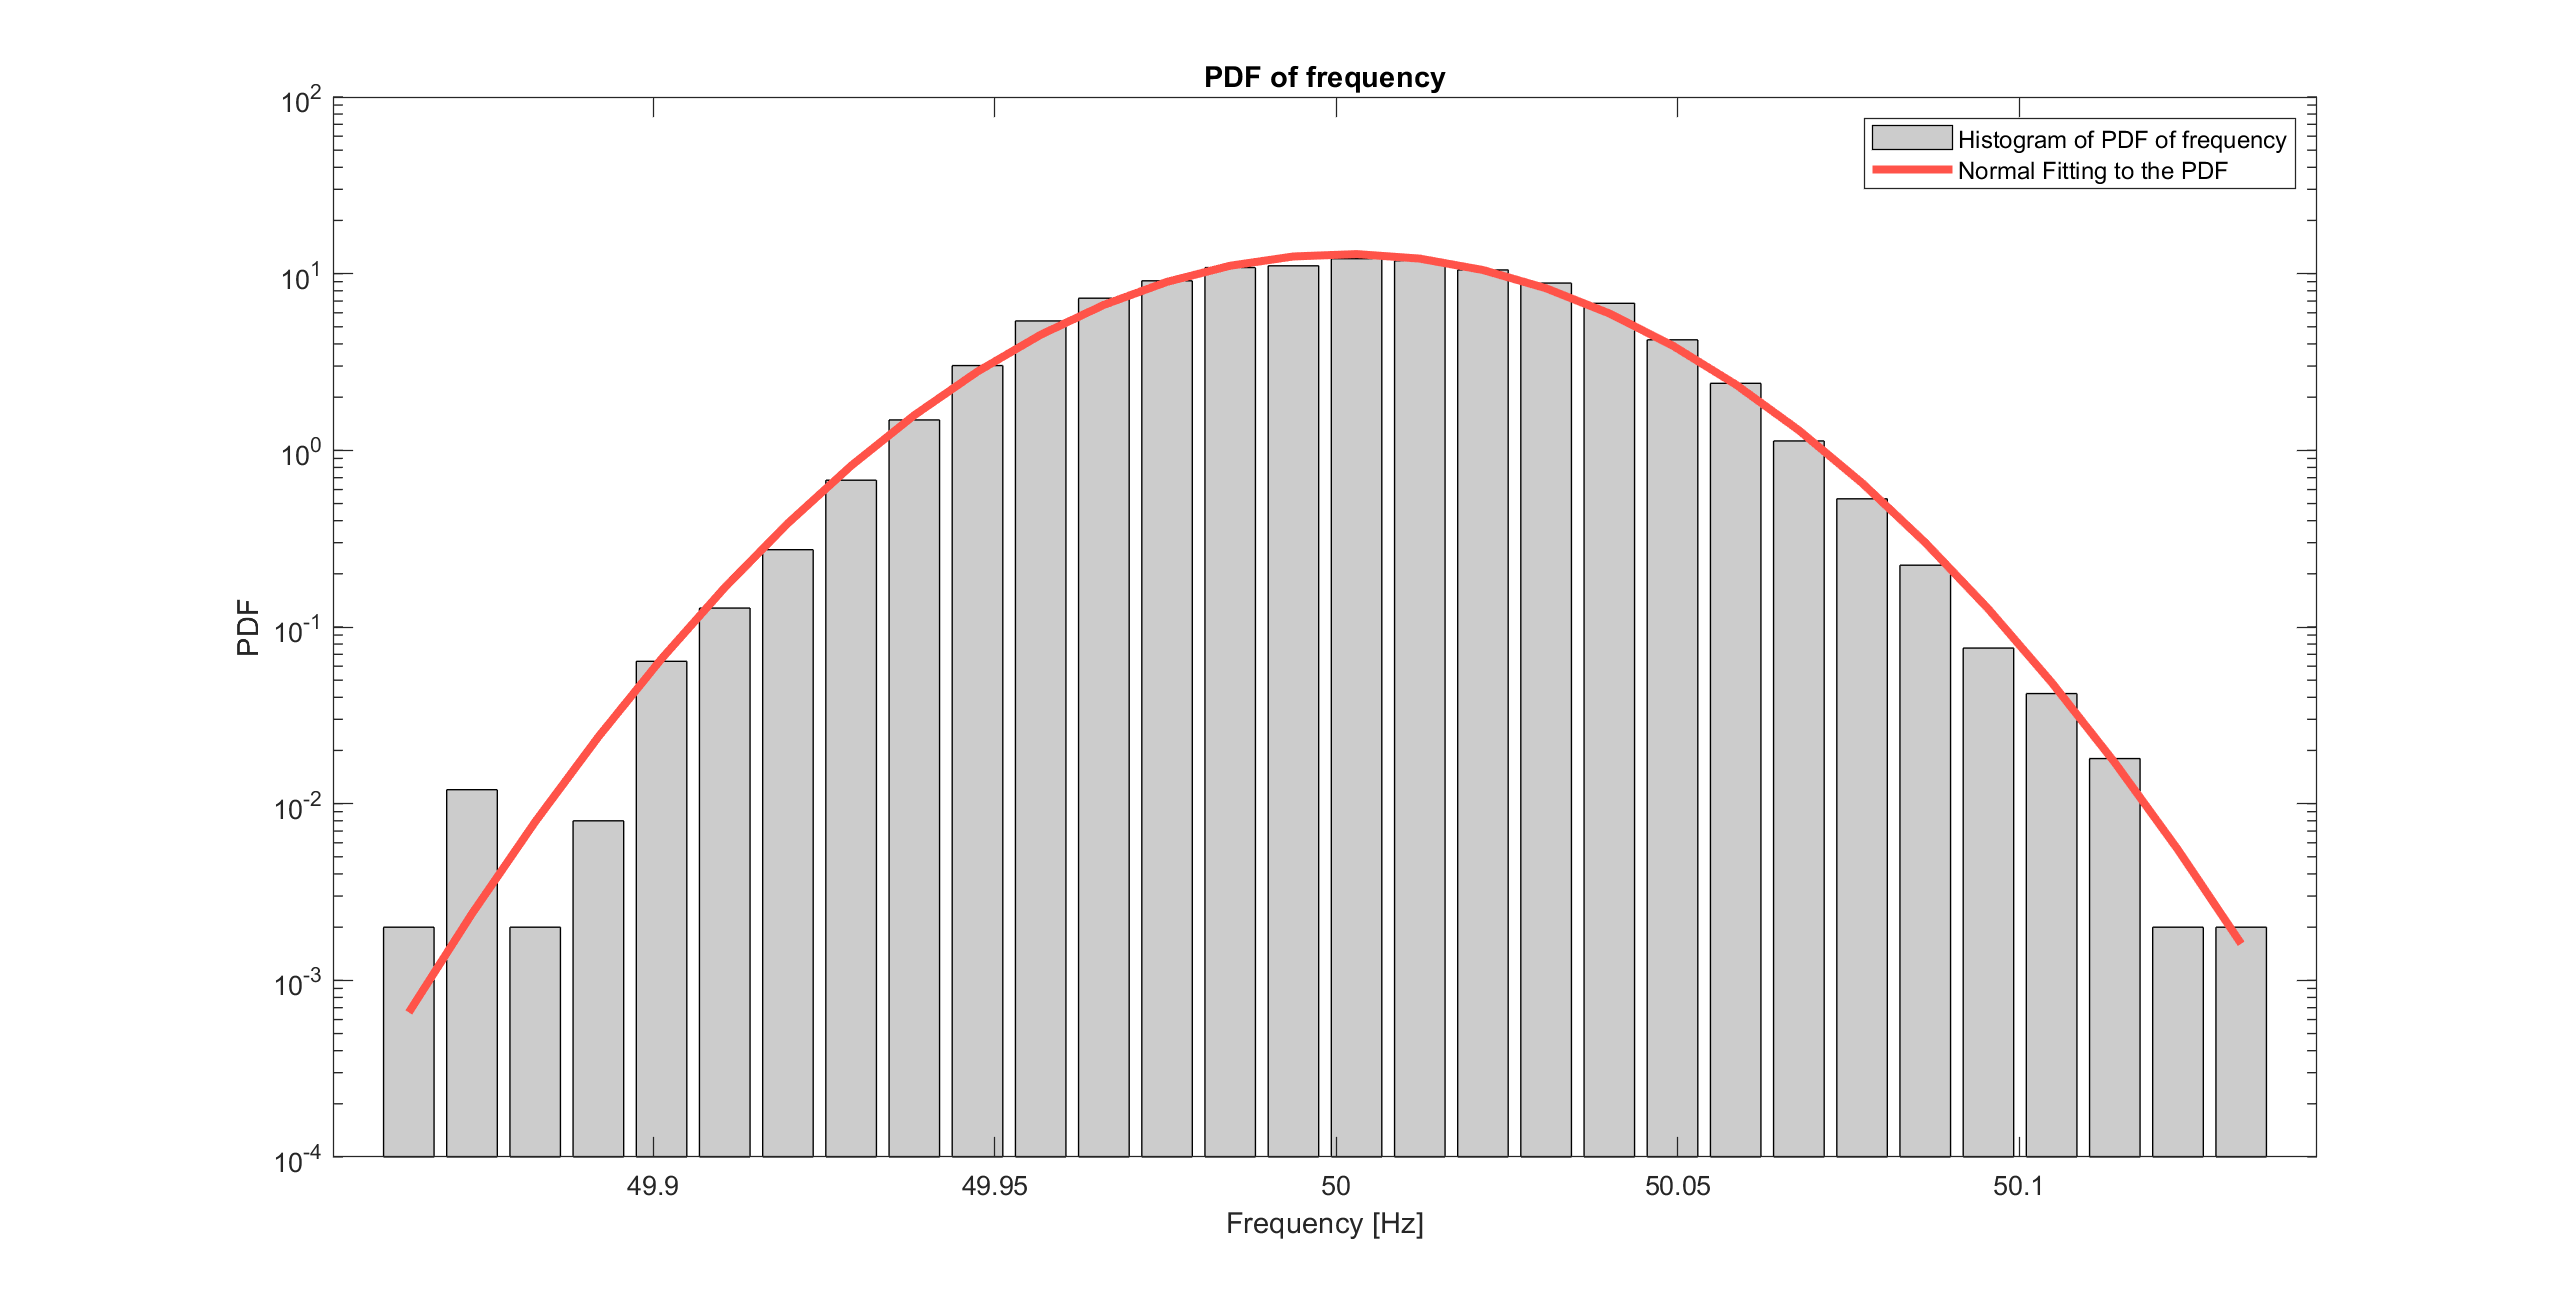
\includegraphics[scale=0.25]{../figures/pdf/pdf_frequency_tokyo_2020_01}
		\caption{Frequency Probability Density Function plots for the Tokyo grid for January 2020.}
	\end{subfigure}

	\begin{subfigure}{\textwidth}
		\centering
		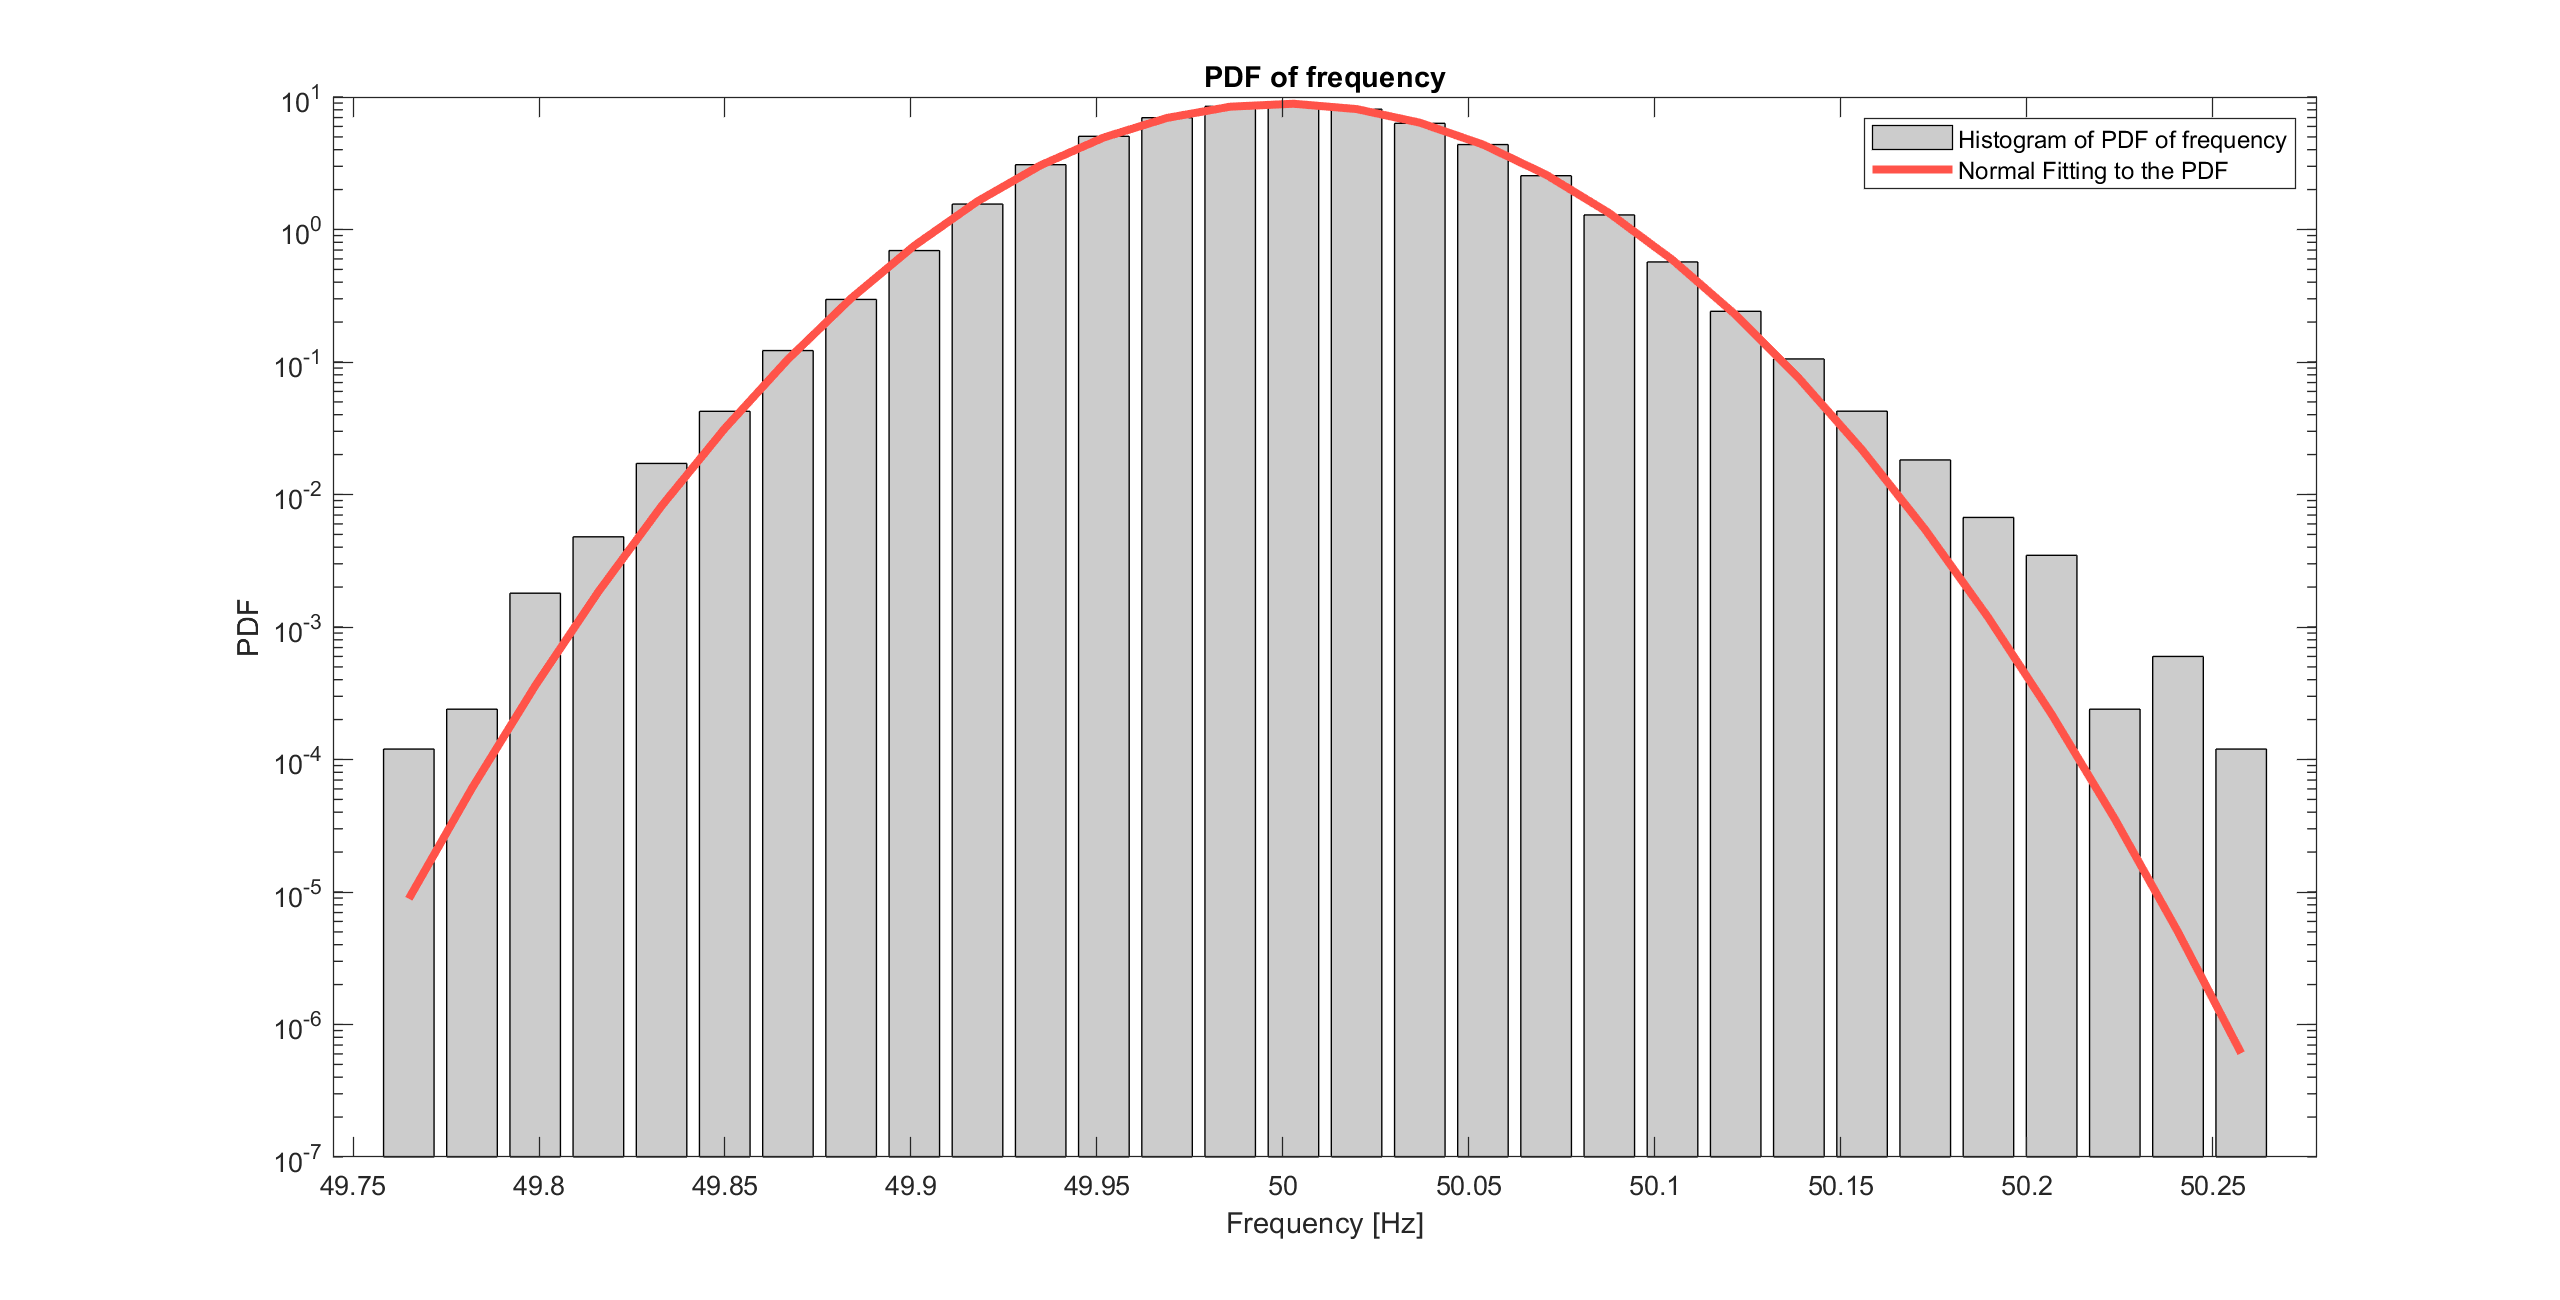
\includegraphics[scale=0.25]{../figures/pdf/pdf_frequency_nordic_2019}
		\caption{Frequency Probability Density Function plots for the Nordic grid for the year 2019.}
	\end{subfigure}
	\caption{Frequency distribution PDFs of some grids show almost identical characteristics to the Gaussian Distribution. For the case of Tokyo and Nordic grids, there is a fair level of agreement between the actual PDF values (grey bars) and the closest fitted Gaussian model (red curve). An assumption of Guassianity, for some grids, therefore is not completely unfounded.}
\end{figure}

\begin{figure}[!ht]
	\centering
	\begin{subfigure}{\textwidth}
		\centering
		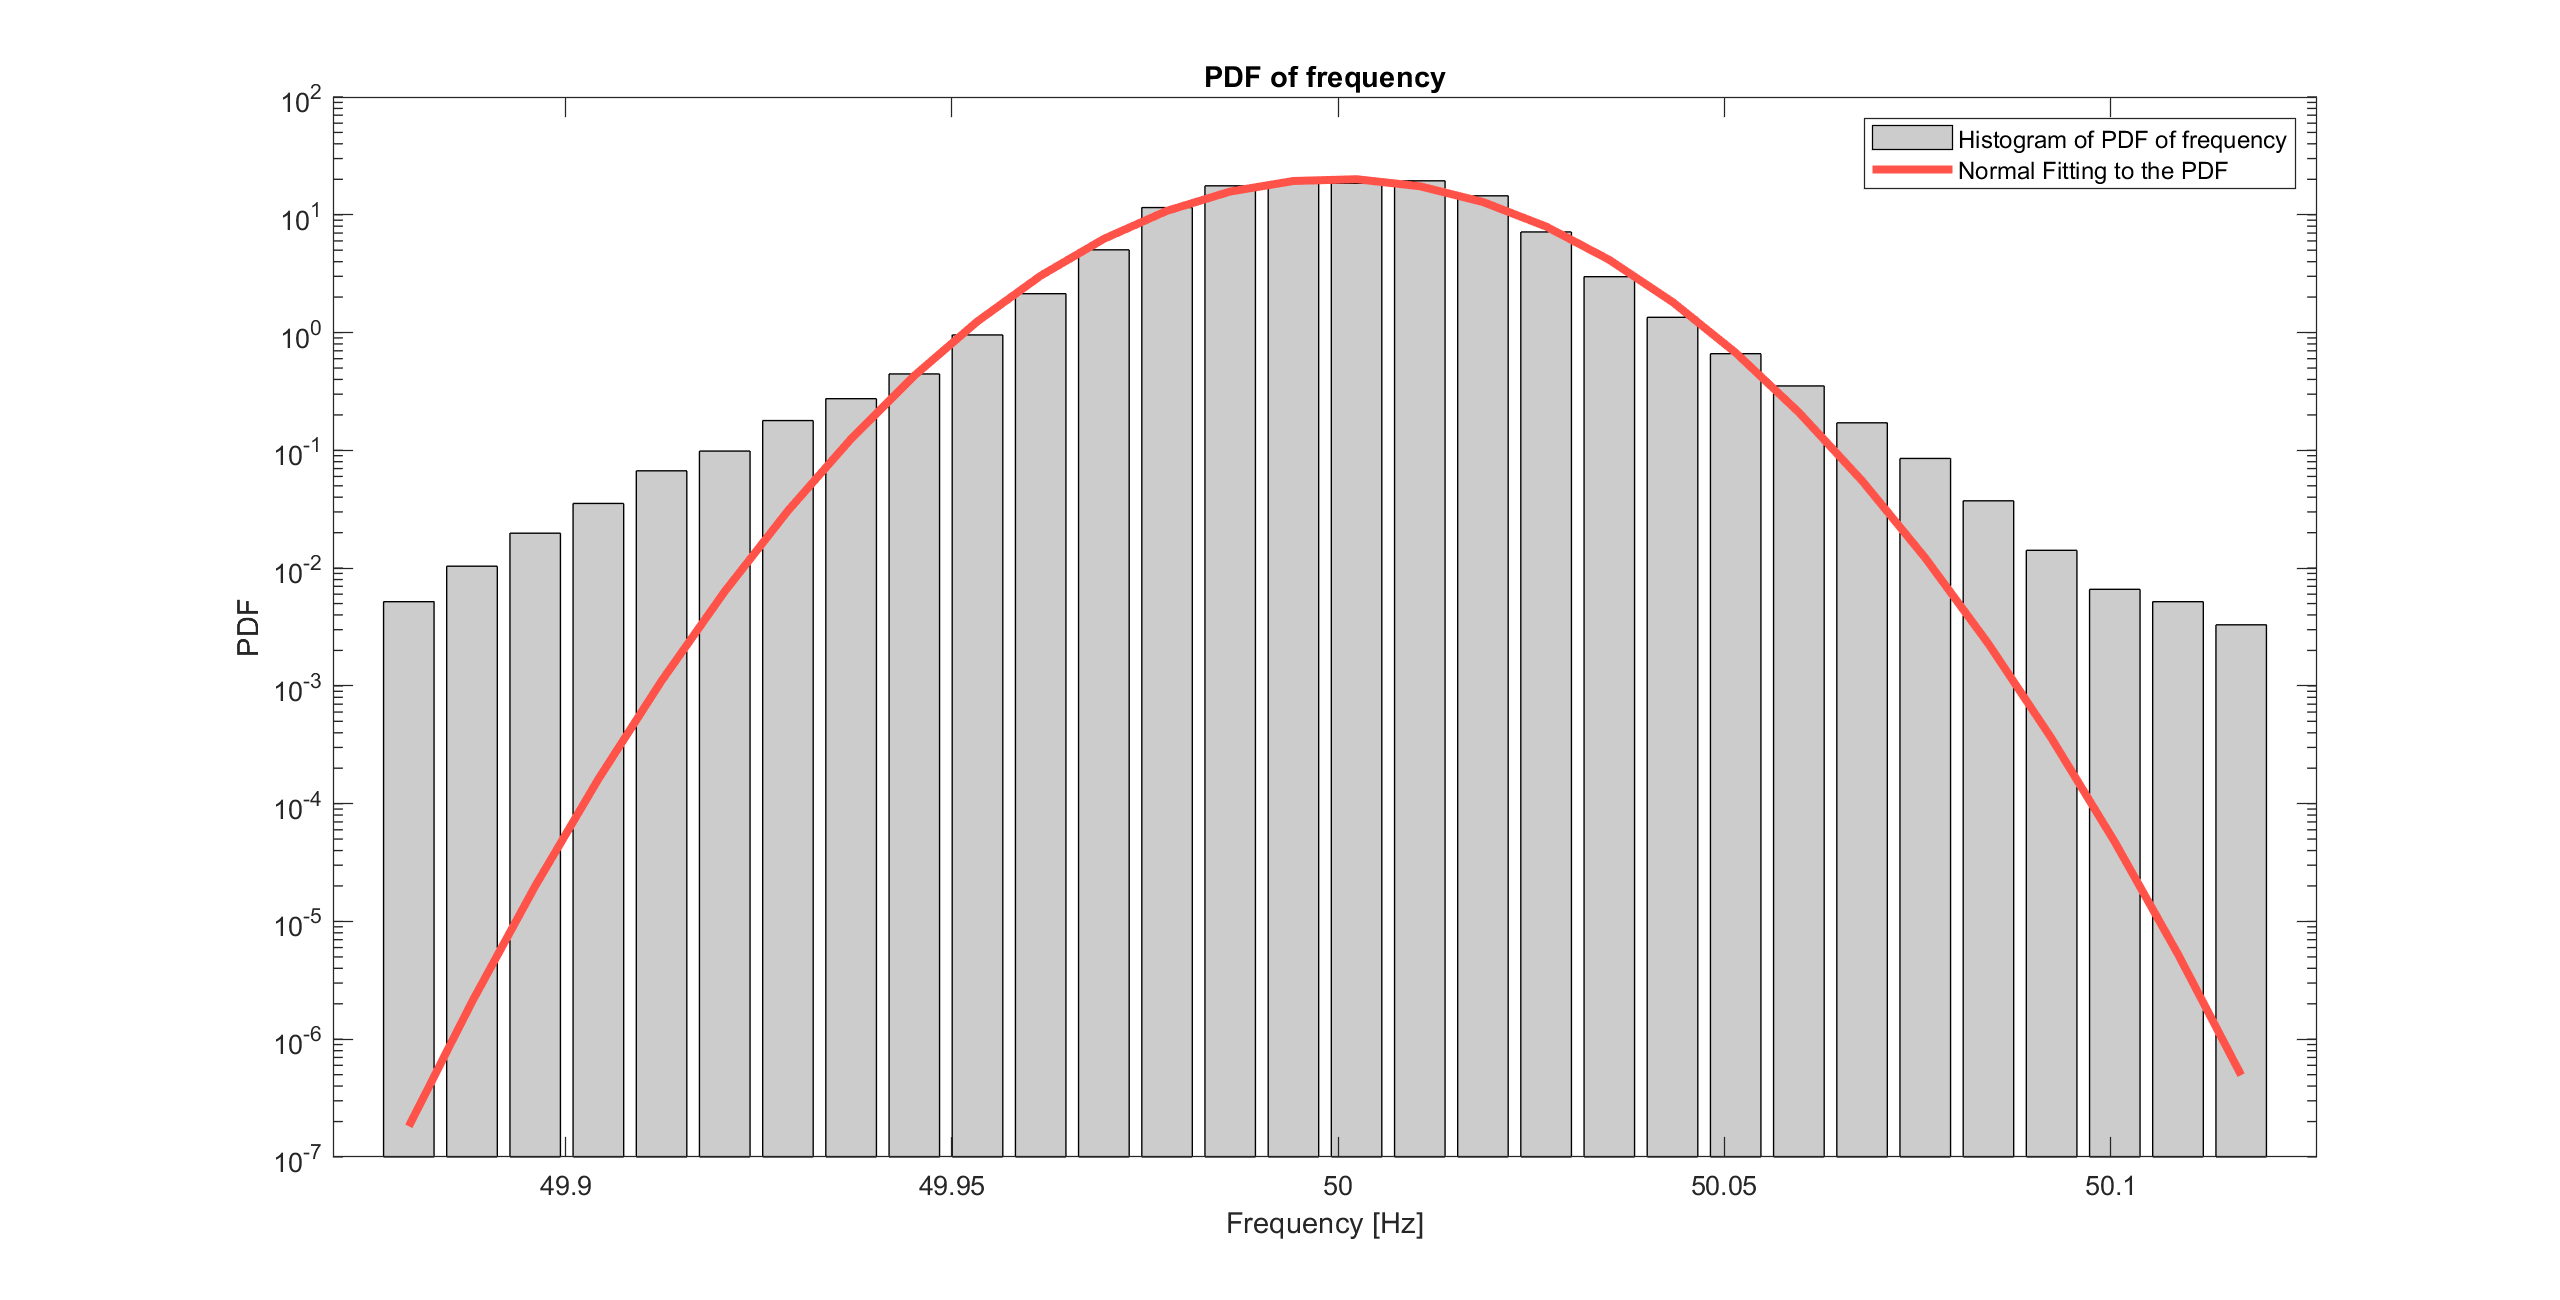
\includegraphics[scale=0.25]{../figures/pdf/pdf_frequency_rte_2019_09}
		\caption{Frequency Probability Density Function plot for the French RTE grid for September 2019.}
	\end{subfigure}
	
	\begin{subfigure}{\textwidth}
		\centering
		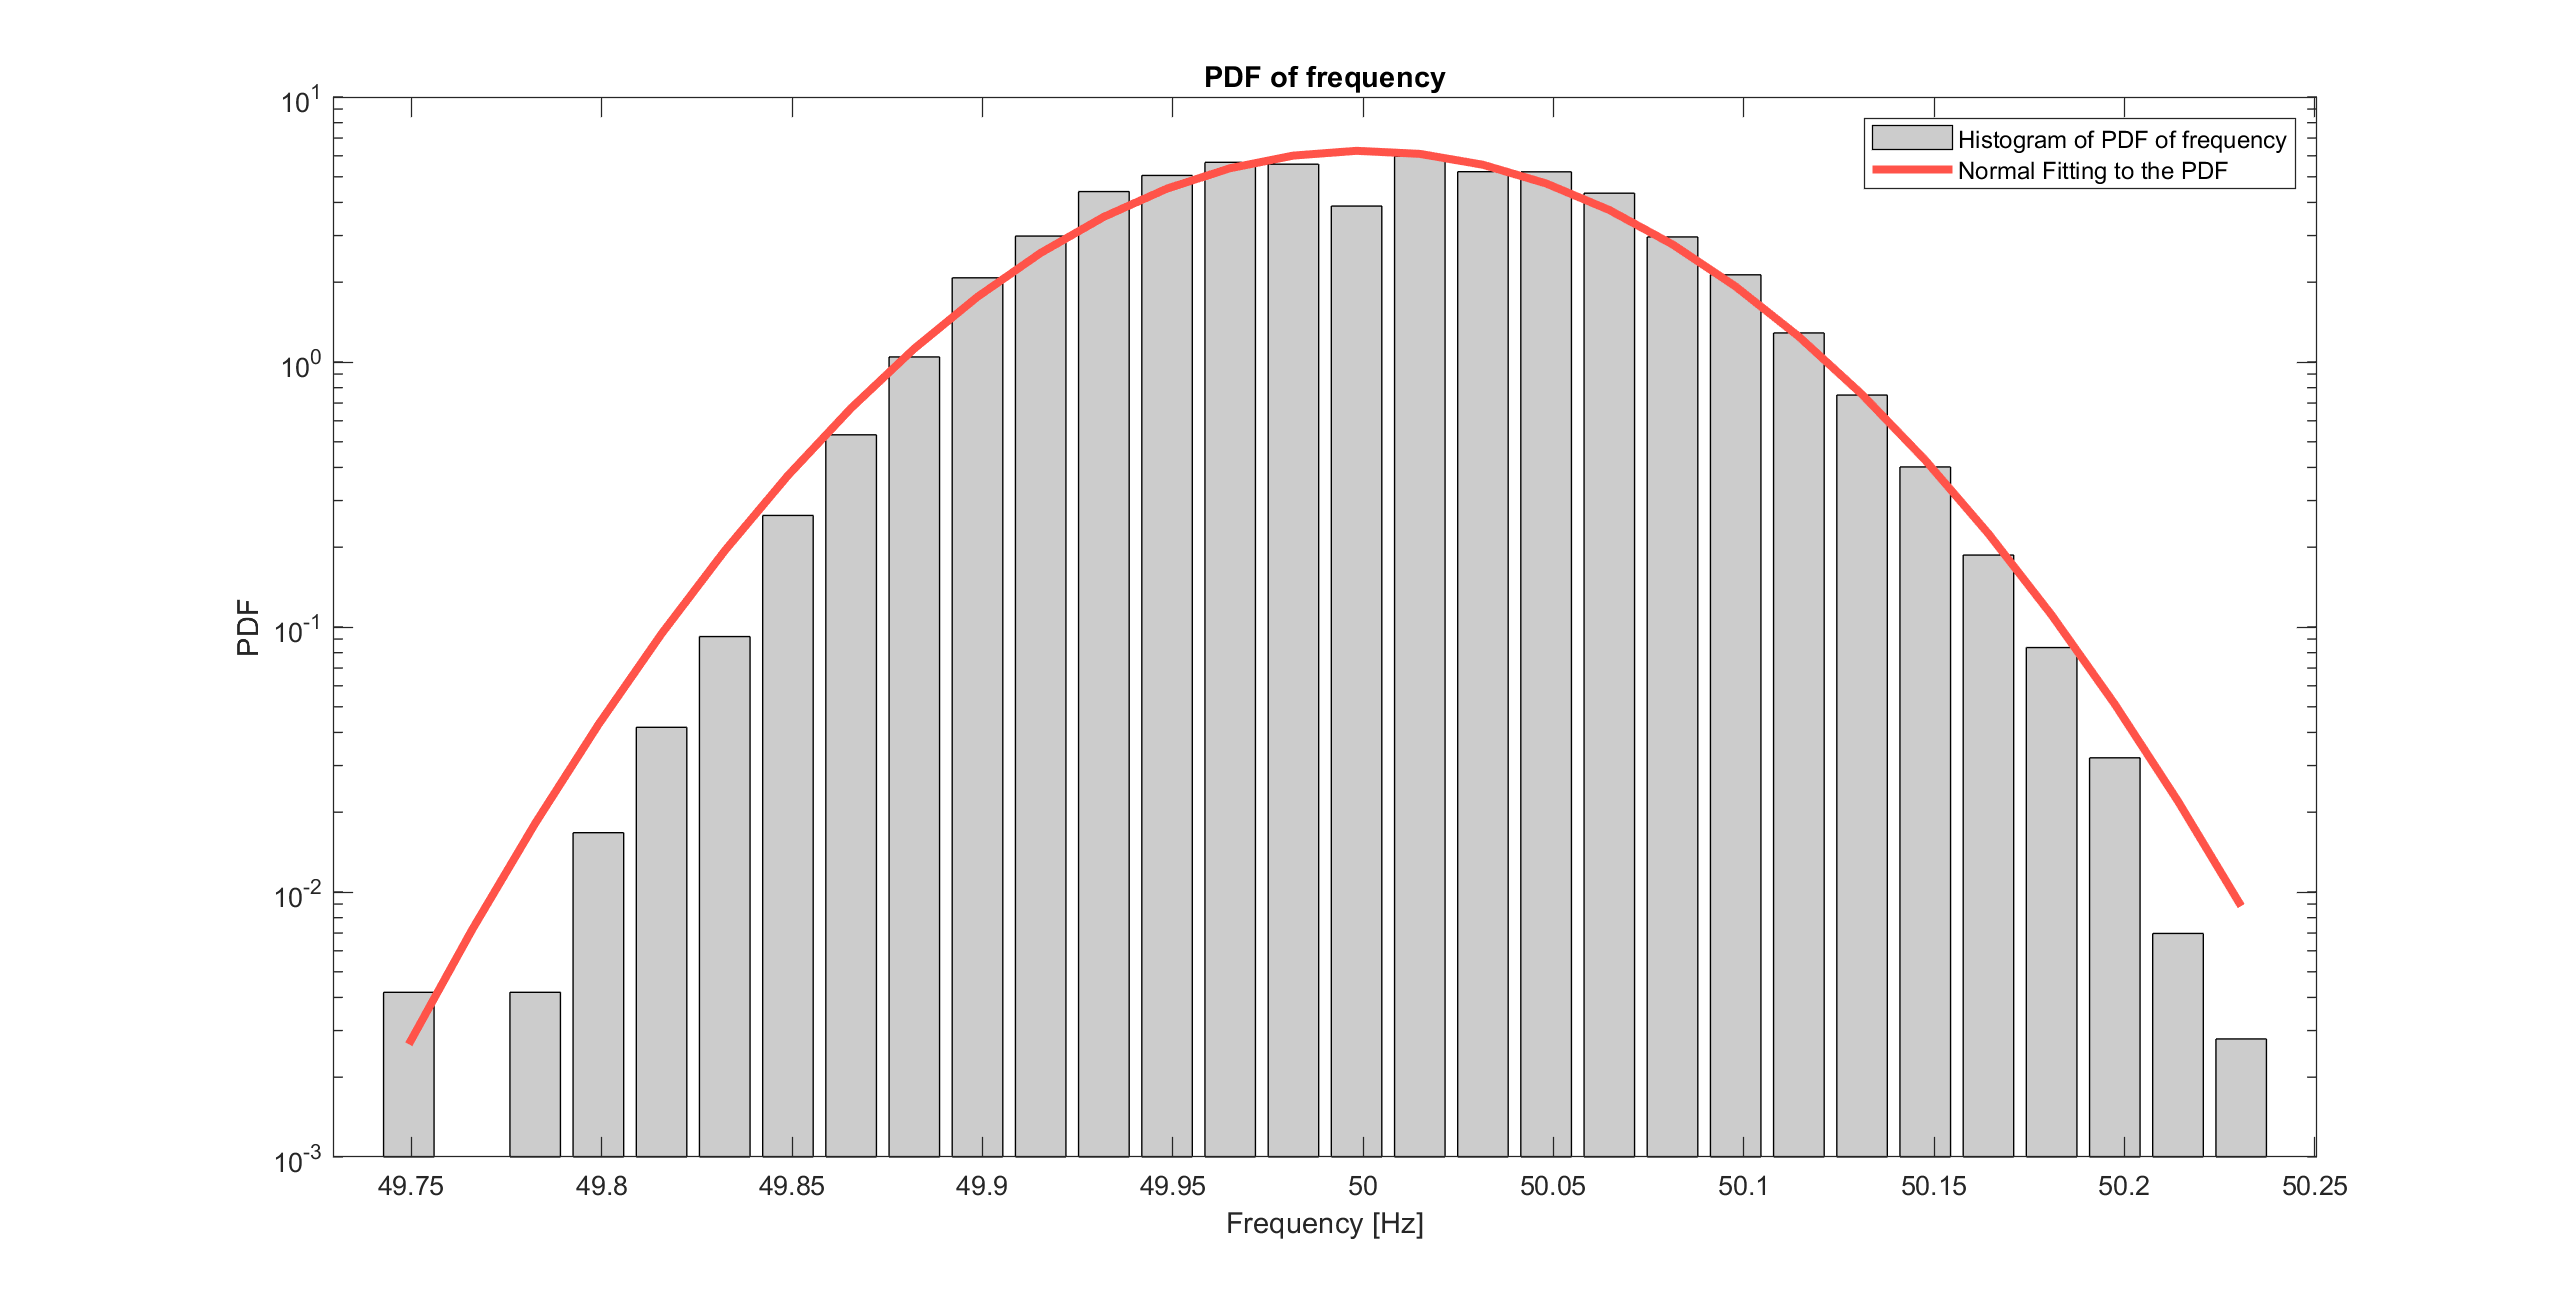
\includegraphics[scale=0.25]{../figures/pdf/pdf_frequency_uk_2020_04}
		\caption{Frequency Probability Density Function plot for the Great Britain grid for April 2020.}
	\end{subfigure}

	\caption{Some sets of grids show an appreciable level of deviation from the Gaussian distribution in that: they have heavier tails, such as for the French RTE Grid, or they have a bimodal distribution (two peaks), such as for the Great Britain Grid.}
\end{figure}

\begin{figure}[!ht]
	\centering
	\begin{subfigure}{\textwidth}
		\centering
		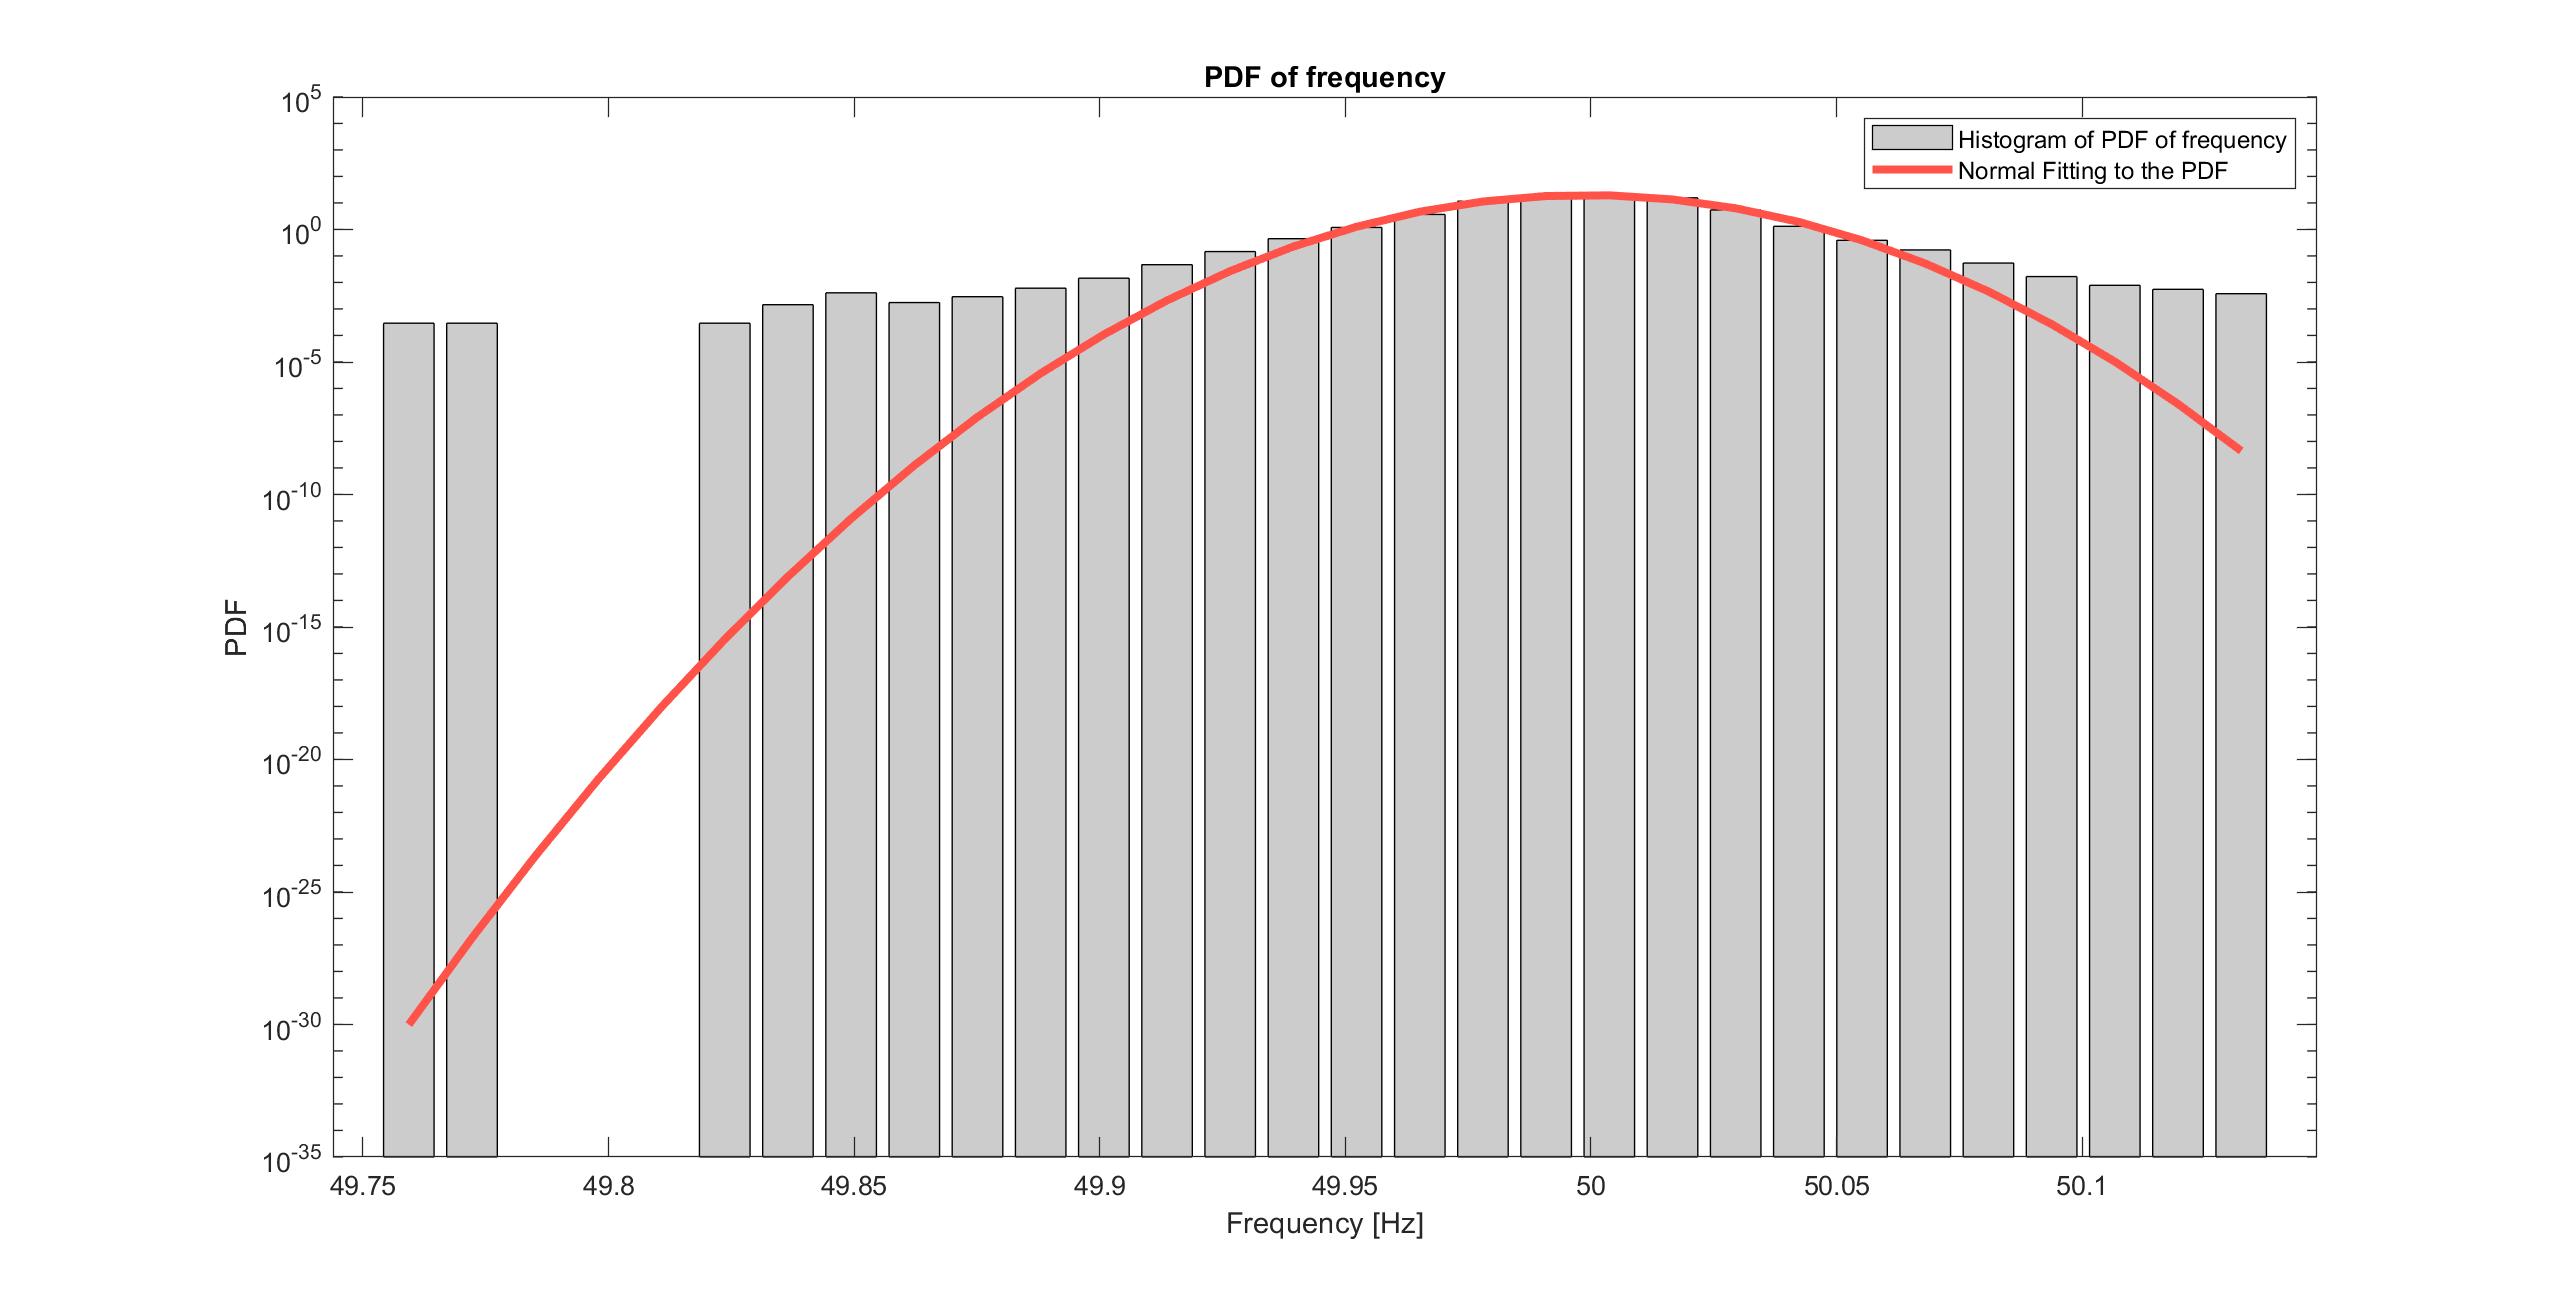
\includegraphics[scale=0.25]{../figures/pdf/pdf_frequency_rte_2021_01_blackout}
		\caption{Frequency Probability Density Function plot for the French RTE grid for January 2021.}
	\end{subfigure}
	
	\begin{subfigure}{\textwidth}
		\centering
		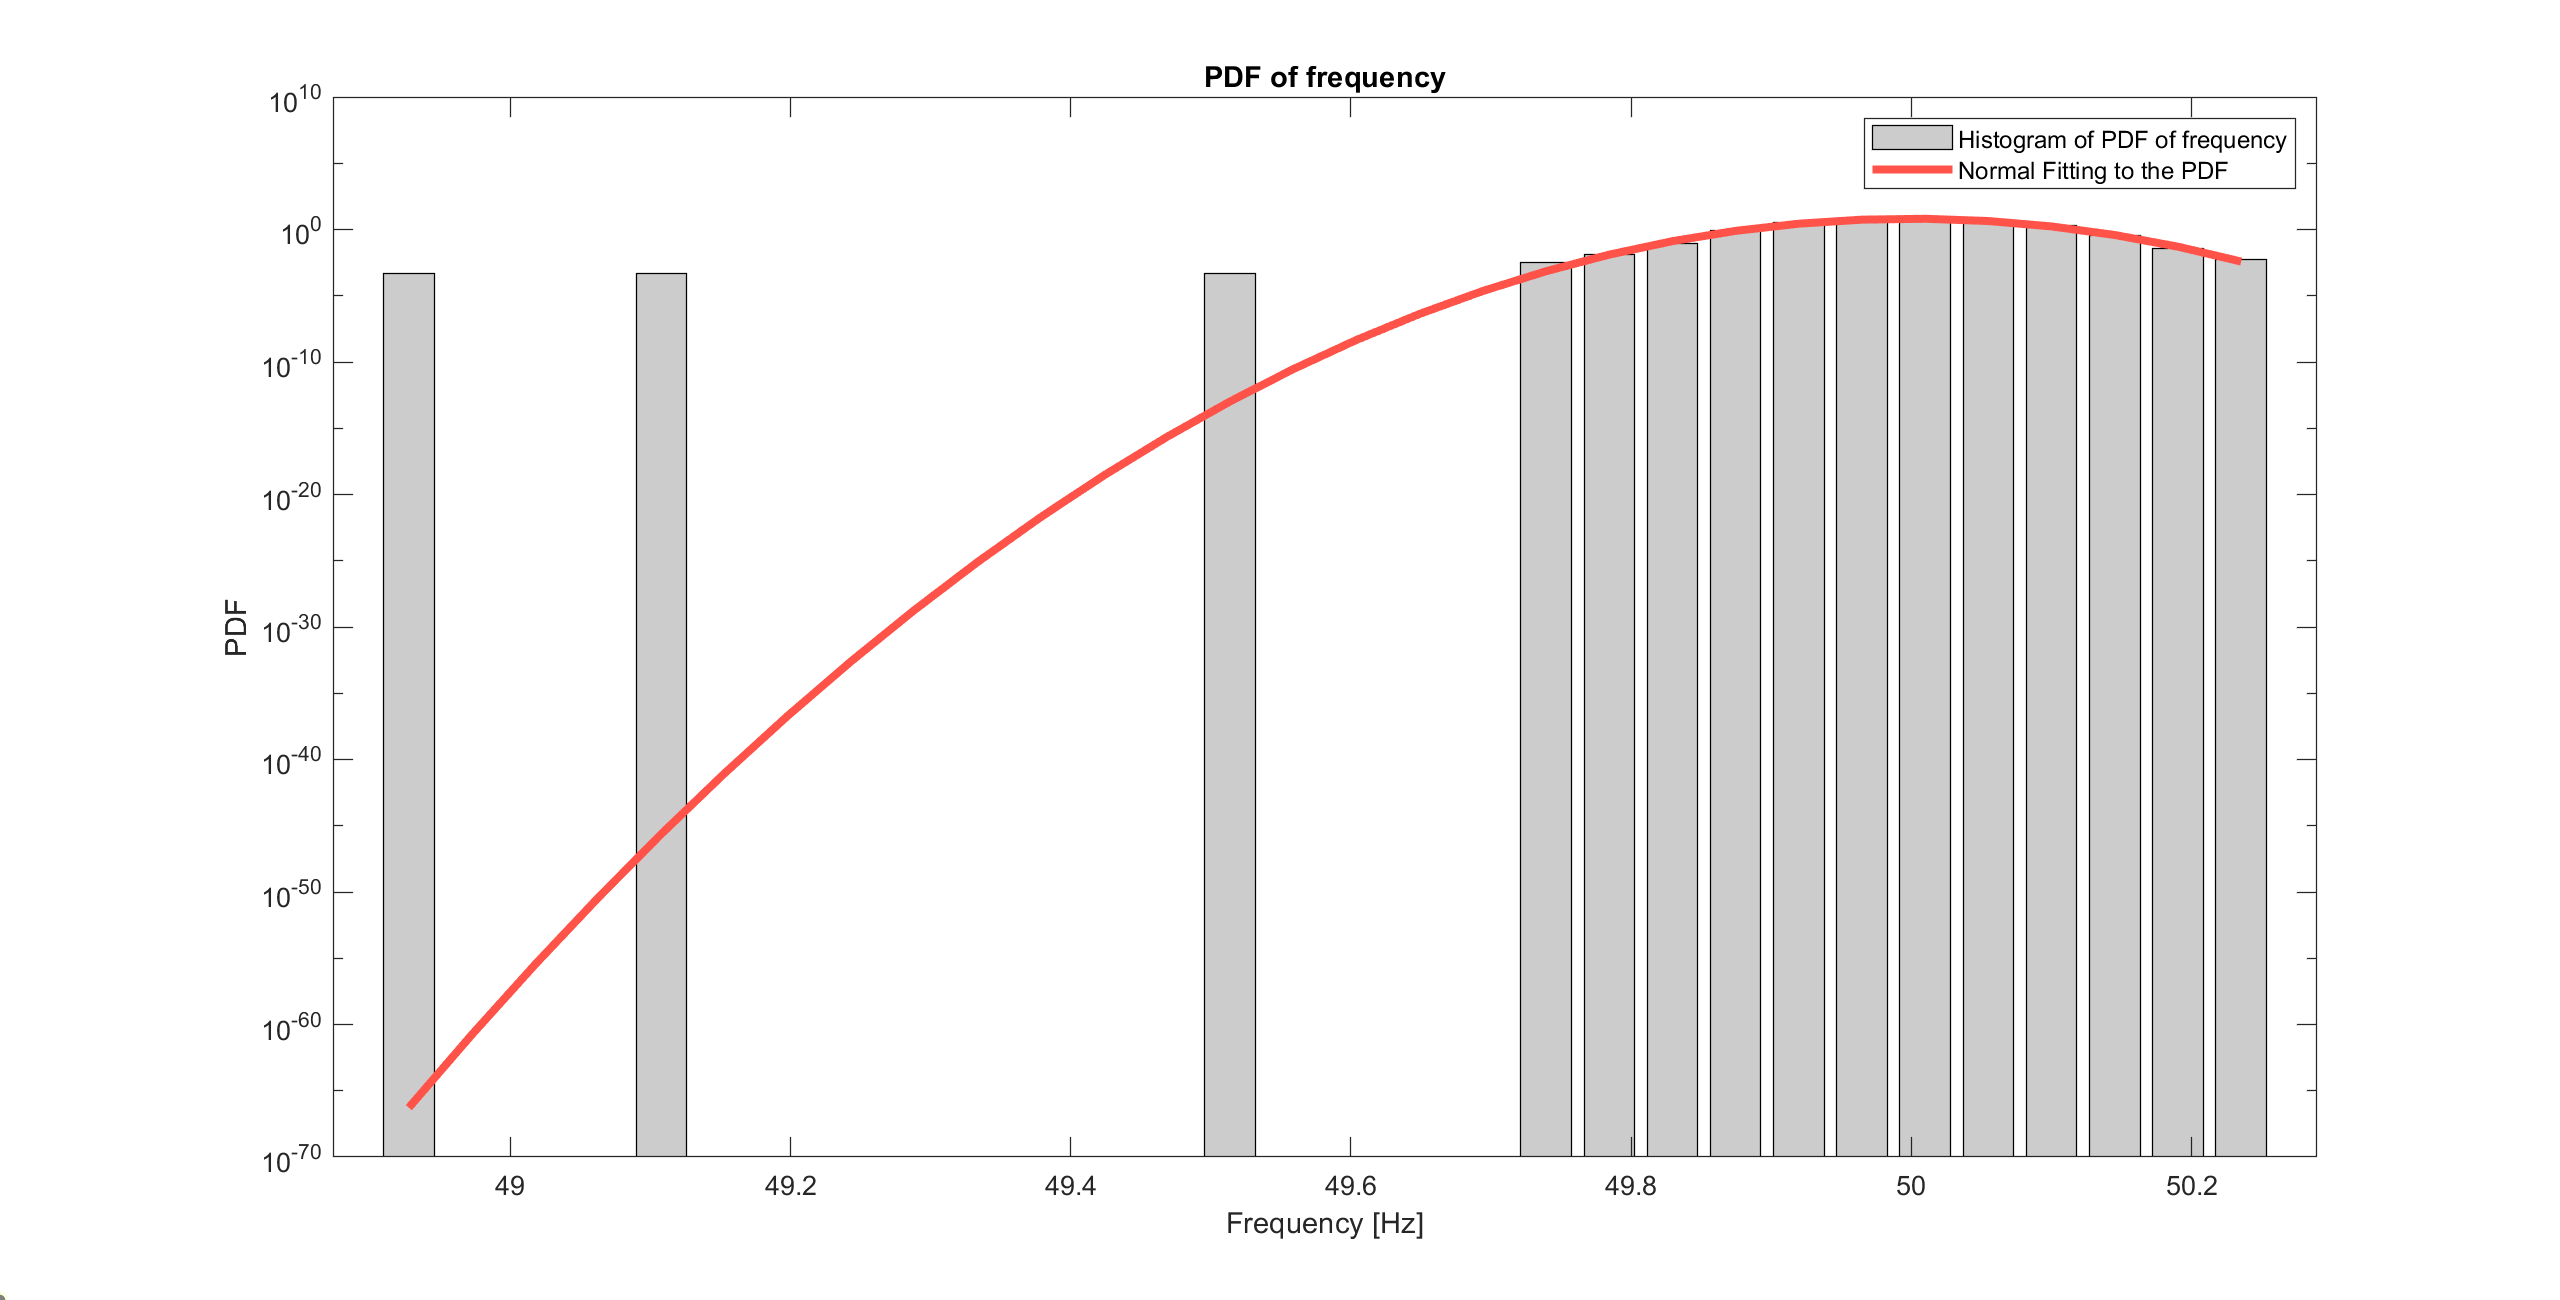
\includegraphics[scale=0.25]{../figures/pdf/pdf_frequency_uk_2019_08_blackout}
		\caption{Frequency Probability Density Function plot for the Great Britain grid for August 2019.}
	\end{subfigure}
	\caption{Blackouts are easily singled out in visual post mortem analysis of grid frequency PDFs. A frequency PDF of a grid plotted for a time duration incorporating a blackout is generally too anomalous from the `usual' non-blackout PDFs. In the above plots, the severe outliers in the PDFs of the French RTE and the Great Britain grids were the results of occurrence of a 10 minute blackout on 08 January 2021 and a 5 minute blackout on 09 August 2019 respectively.}
\end{figure}

\begin{figure}[!ht]
	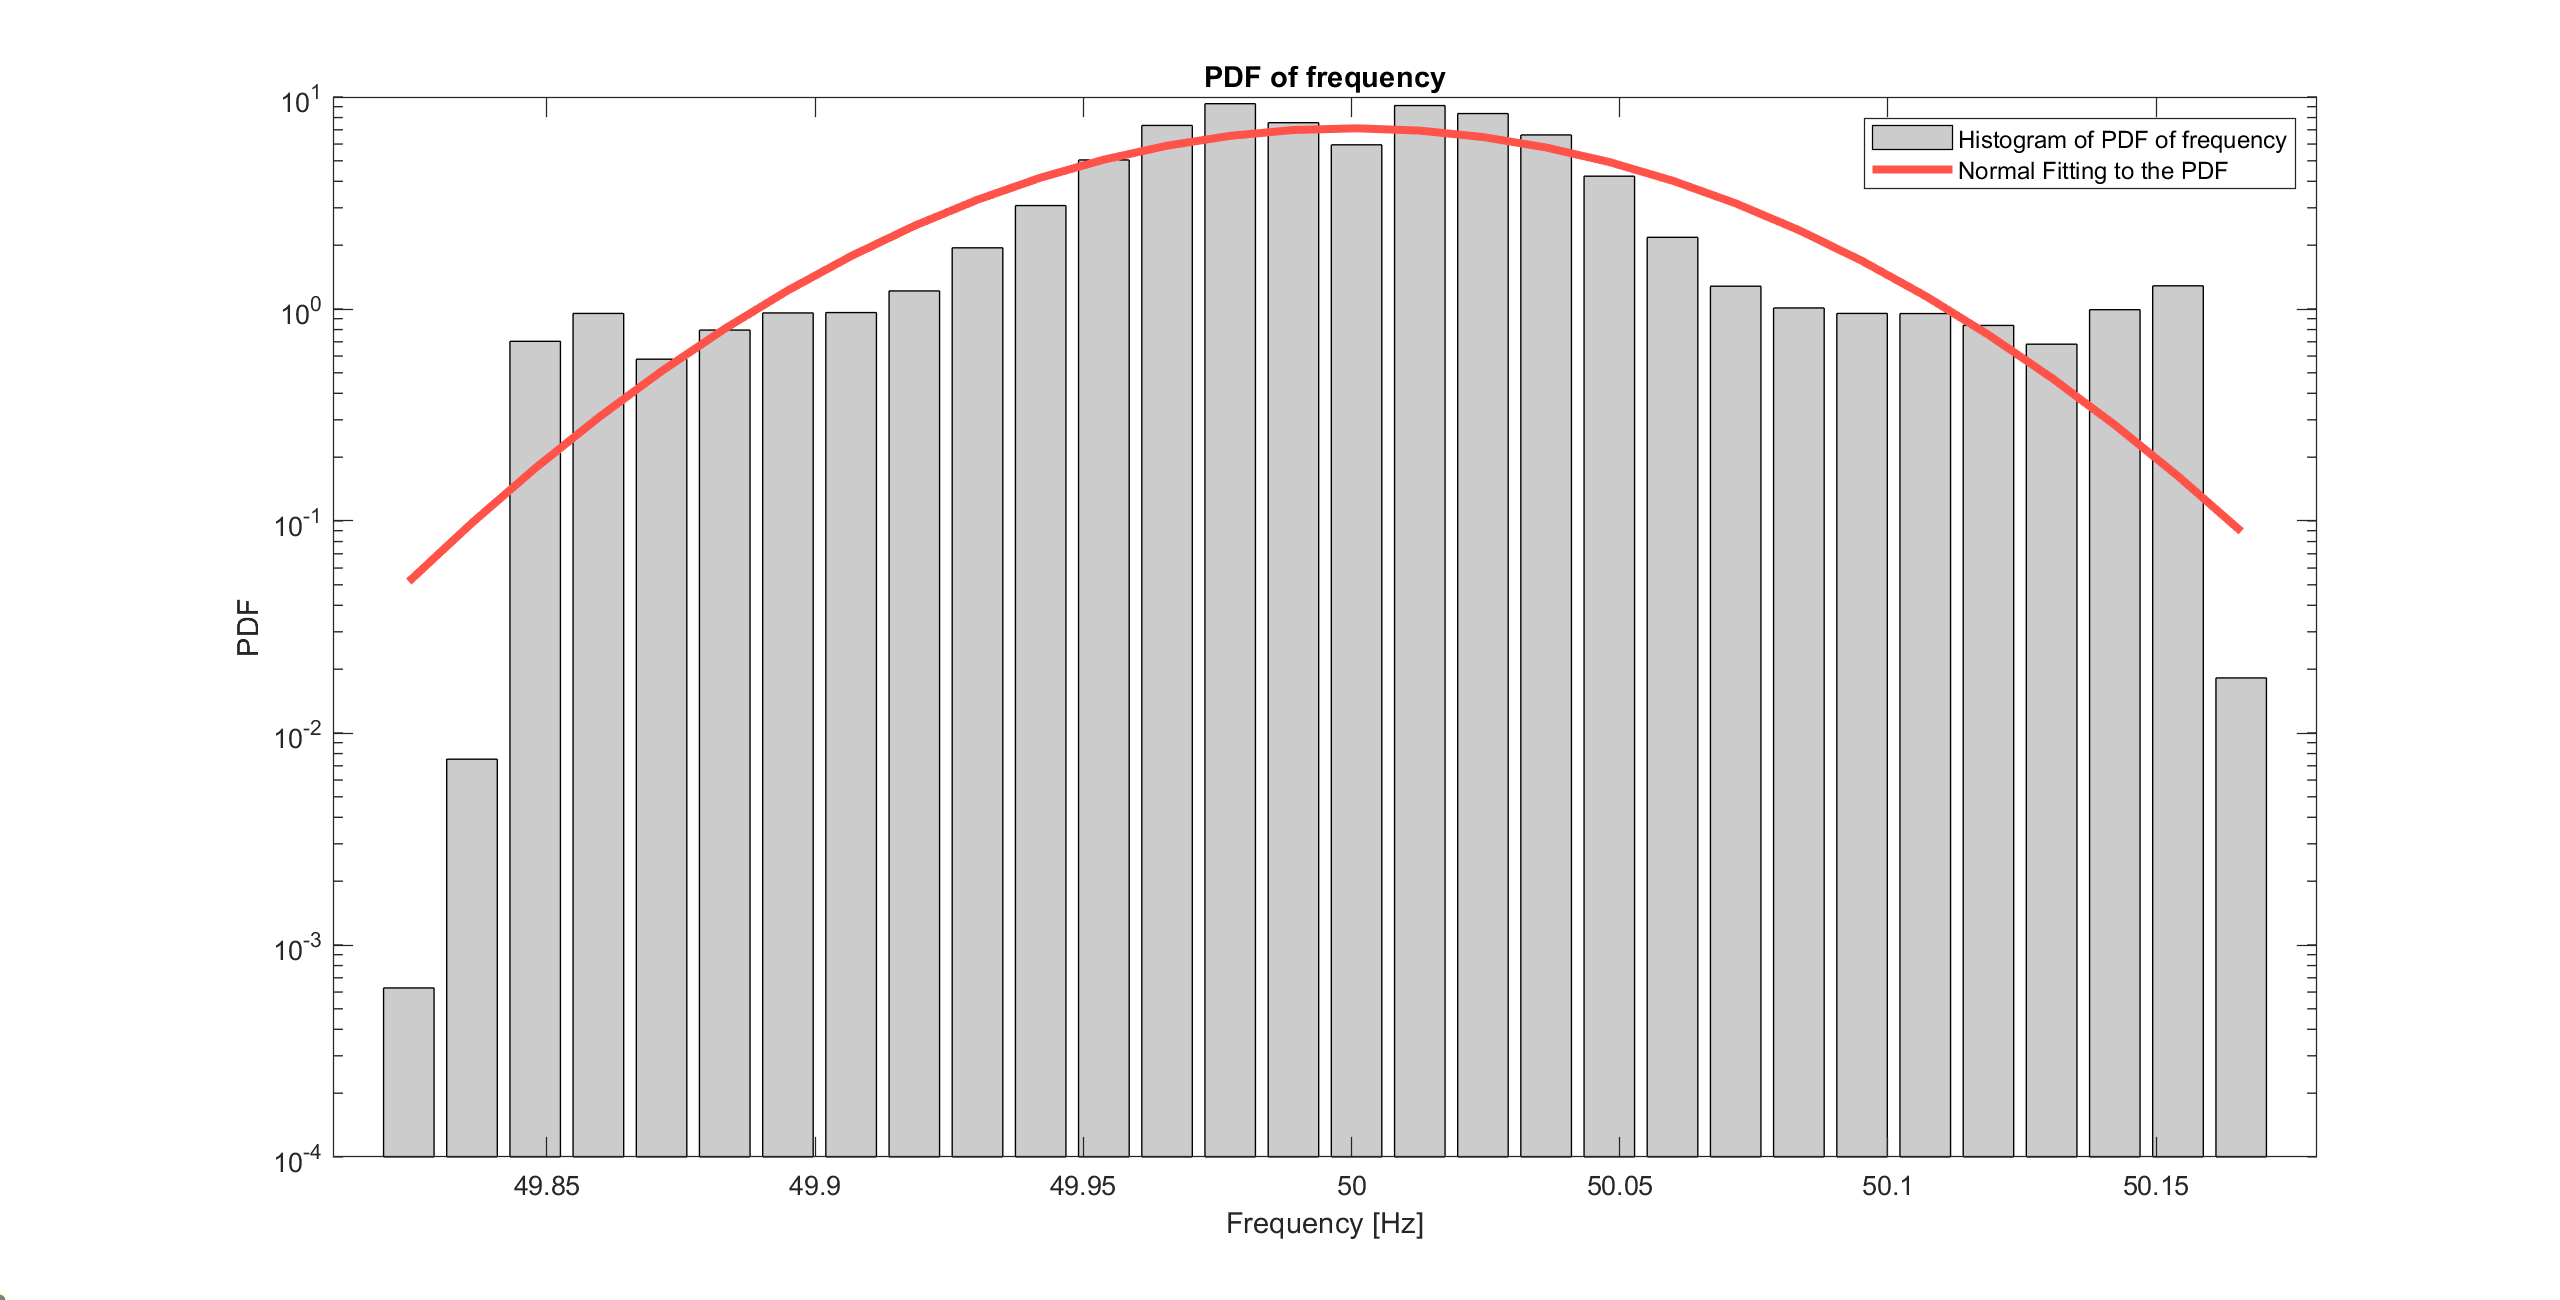
\includegraphics[scale=0.25]{../figures/pdf/pdf_frequency_spain_mallorca_2019_05_f1}
	\caption{Frequency Probability Density Function plots for the Spanish Mallorcan grid for the May 2019. There is high degree of deviation of the actual PDF values (grey bars) from the closest Gaussian model fitted to the same data (red curve). Apart from the heavier tails, the frequency distribution appears to have multiple peaks.}
\end{figure}


The plotted bulk distribution PDFs visually revealed insights including any deadbands \cite{francesca01, vorobev01} mandated in their grid operation, their skewness, thickness of their tails, etc. A quantitative study of their moments like kurtosis and skewness was not conducted as was done in \cite{schafer01}.

\begin{figure}[ht]
	\centering
	\resizebox{0.75\linewidth}{!}{\import{../figures/autocorr}{comparison_five_no_title.tex}}
	\caption{Fixed Time Autocorrelation plots for five different power grids. The different rates of exponential decay in autocorrelation values indicates the difference in their relative damping strengths. The Continental European and Great Britain grids display peaks every $15$ minutes which may be explained from their energy dispatch routine.}
	\label{fig:comp5}
\end{figure}

In the plotted autocorrelation decay curves, all grids showed exponentially decreasing autocorrelations $c(\tau$) for smaller values of $\tau$. 

\begin{equation}
	c(\tau) \propto exp{\left(-\frac{\tau}{t_{corr}}\right)}
\end{equation}

where $t_{corr}$ is the correlation constant for the grid (the time period in which autocorrelation decays to $\frac{1}{e}$th of its original value). This is in agreement with the usual autocorrelation decay trends observed for natural stochastic processes, such as the Ornstein-Uhlenbeck Process \cite{numericalSolutionForStochasticDifferentailEquationsKloedenEckhard}. 
Instead of the autocorrelation decay constant $t_{corr}$, sometimes its reciprocal, inverse-time autocorrelation decay constant $\frac{1}{t_{corr}}$ or simply $t_{corr}^{-1}$ is used.   
In order to confirm if the decrease was indeed exponential with a grid-specific inverse-time autocorrelation decay constant, semi-log graphs ($\log(c(\tau))$ vs $\tau$) were also plotted. The decay constants were computed by calculating the slopes of the semi-log graphs and it was found that the grids which were bigger, more robust and showed bulk distribution PDFs which were less-deviating from Gaussian distributions, had greater values of inverse-time correlation ${t_{corr}}^{-1}$. This parameter can also be construed as $\alpha$, the relative damping strength of the grid for small oscillations and can be an indicator of the overall robustness of the grid. Refer to Table \ref{tab:invCorr} for the computed values.

\documentclass[varwidth=\maxdimen]{standalone}
\usepackage{tabularx}
\usepackage{textcomp}
\usepackage{booktabs}

\begin{document}
	\begin{table}[h]
		\caption{Inverse-correlation values for different grids}
		\centering
		\label{tab:invCorr}
		\begin{tabular}{ c  c}
			\toprule
			Grid name & Inverse-correlation value $T^{-1}$ $[min^{-1}]$\\[0pt]
			\midrule
			Mallorca & $0.0654$\\[0pt]
	
			Western Interconnection & $0.0498$\\[0pt]

			Nordic & $0.0235$\\[0pt]
	
			Continental Europe & $0.0829$\\[0pt]

			Great Britain & $0.0879$\\[0pt]
			\bottomrule			
		\end{tabular}
	\end{table}
\end{document}

\subsection*{Effect of sampling duration on consistency of offline analysis of data}
\label{app:effectOfSamplingDuration}

Different grids can have their own set of `events', such as firing up of boilers or other kinds of switching events, or `cycles' of changes, such as sub-hourly power dispatches, semi-diurnal variation in solar generation, hourly wind power fluctuations, etc. A question then arises: Can the `statistical nature' of a grid be really generalized if it itself doesn't show a constant characteristic in its dynamics? The answer is: Yes, but only if a `sufficient' duration of data has been collected for analysis, such that all kinds of cyclical variations are `averaged-out' over the duration, displaying a somewhat consistent statistical signature irrespective of the actual time the analysis was made or data collected from.

Data for different years or months of select grids (Great Britain, France RTE, Nordic, Japan) mentioned in Table \ref{tab:realGridSamplingData} were compared in terms of their Fixed Time Autocorrelation plots (Autocorrelation Decay Curves). The plots were a mixture of year-wise (Nordic), month-wise (Great Britain, France RTE, Tokyo) and day-wise (Indian NRLDC) data. It was concluded that, barring some small vertical shifts among the autocorrelation values, the trends were consistently displayed for year-wise and month-wise plots, but did not show consistency in their day-to-day plots. 

\begin{figure}[!ht]
	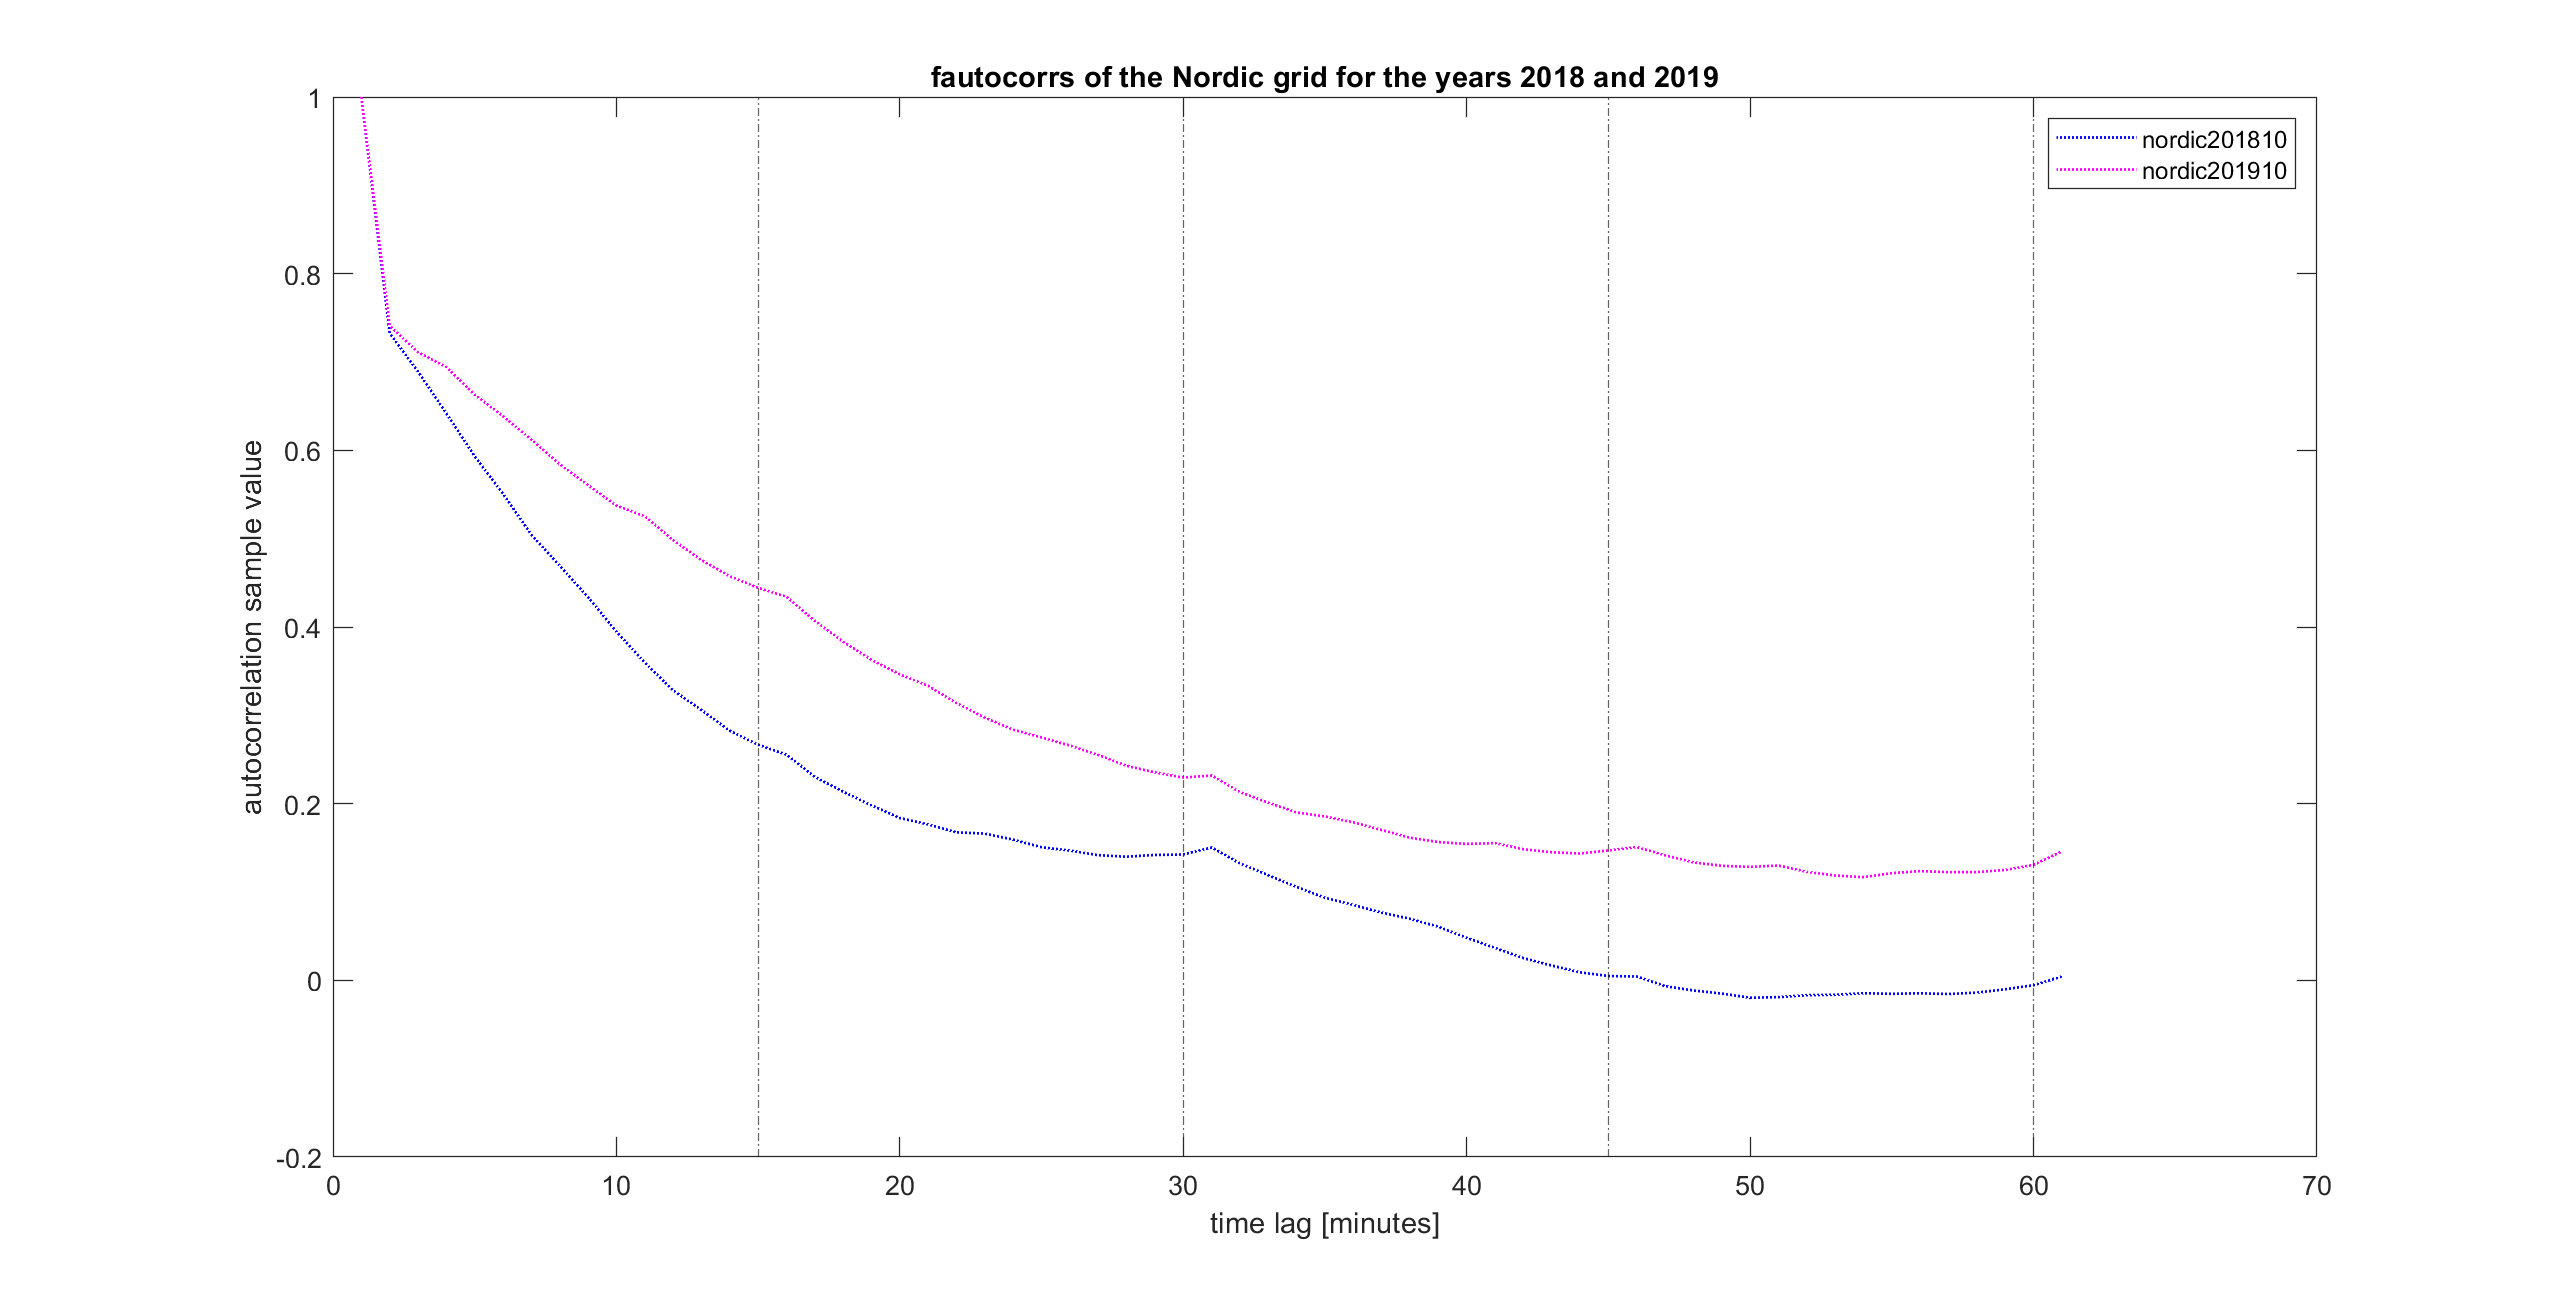
\includegraphics[scale=0.25]{../figures/autocorr/fautocorrs_nordic_201801_to_201912}
	\caption{Fixed Time Autocorrelation plots for the Nordic Grid for two consecutive years, 2018 and 2019. They present a fairly consistent picture of the grid's dynamics, with only a minor difference in the magnitude of the autocorrelation values.}
\end{figure}


\begin{figure}[!ht]
	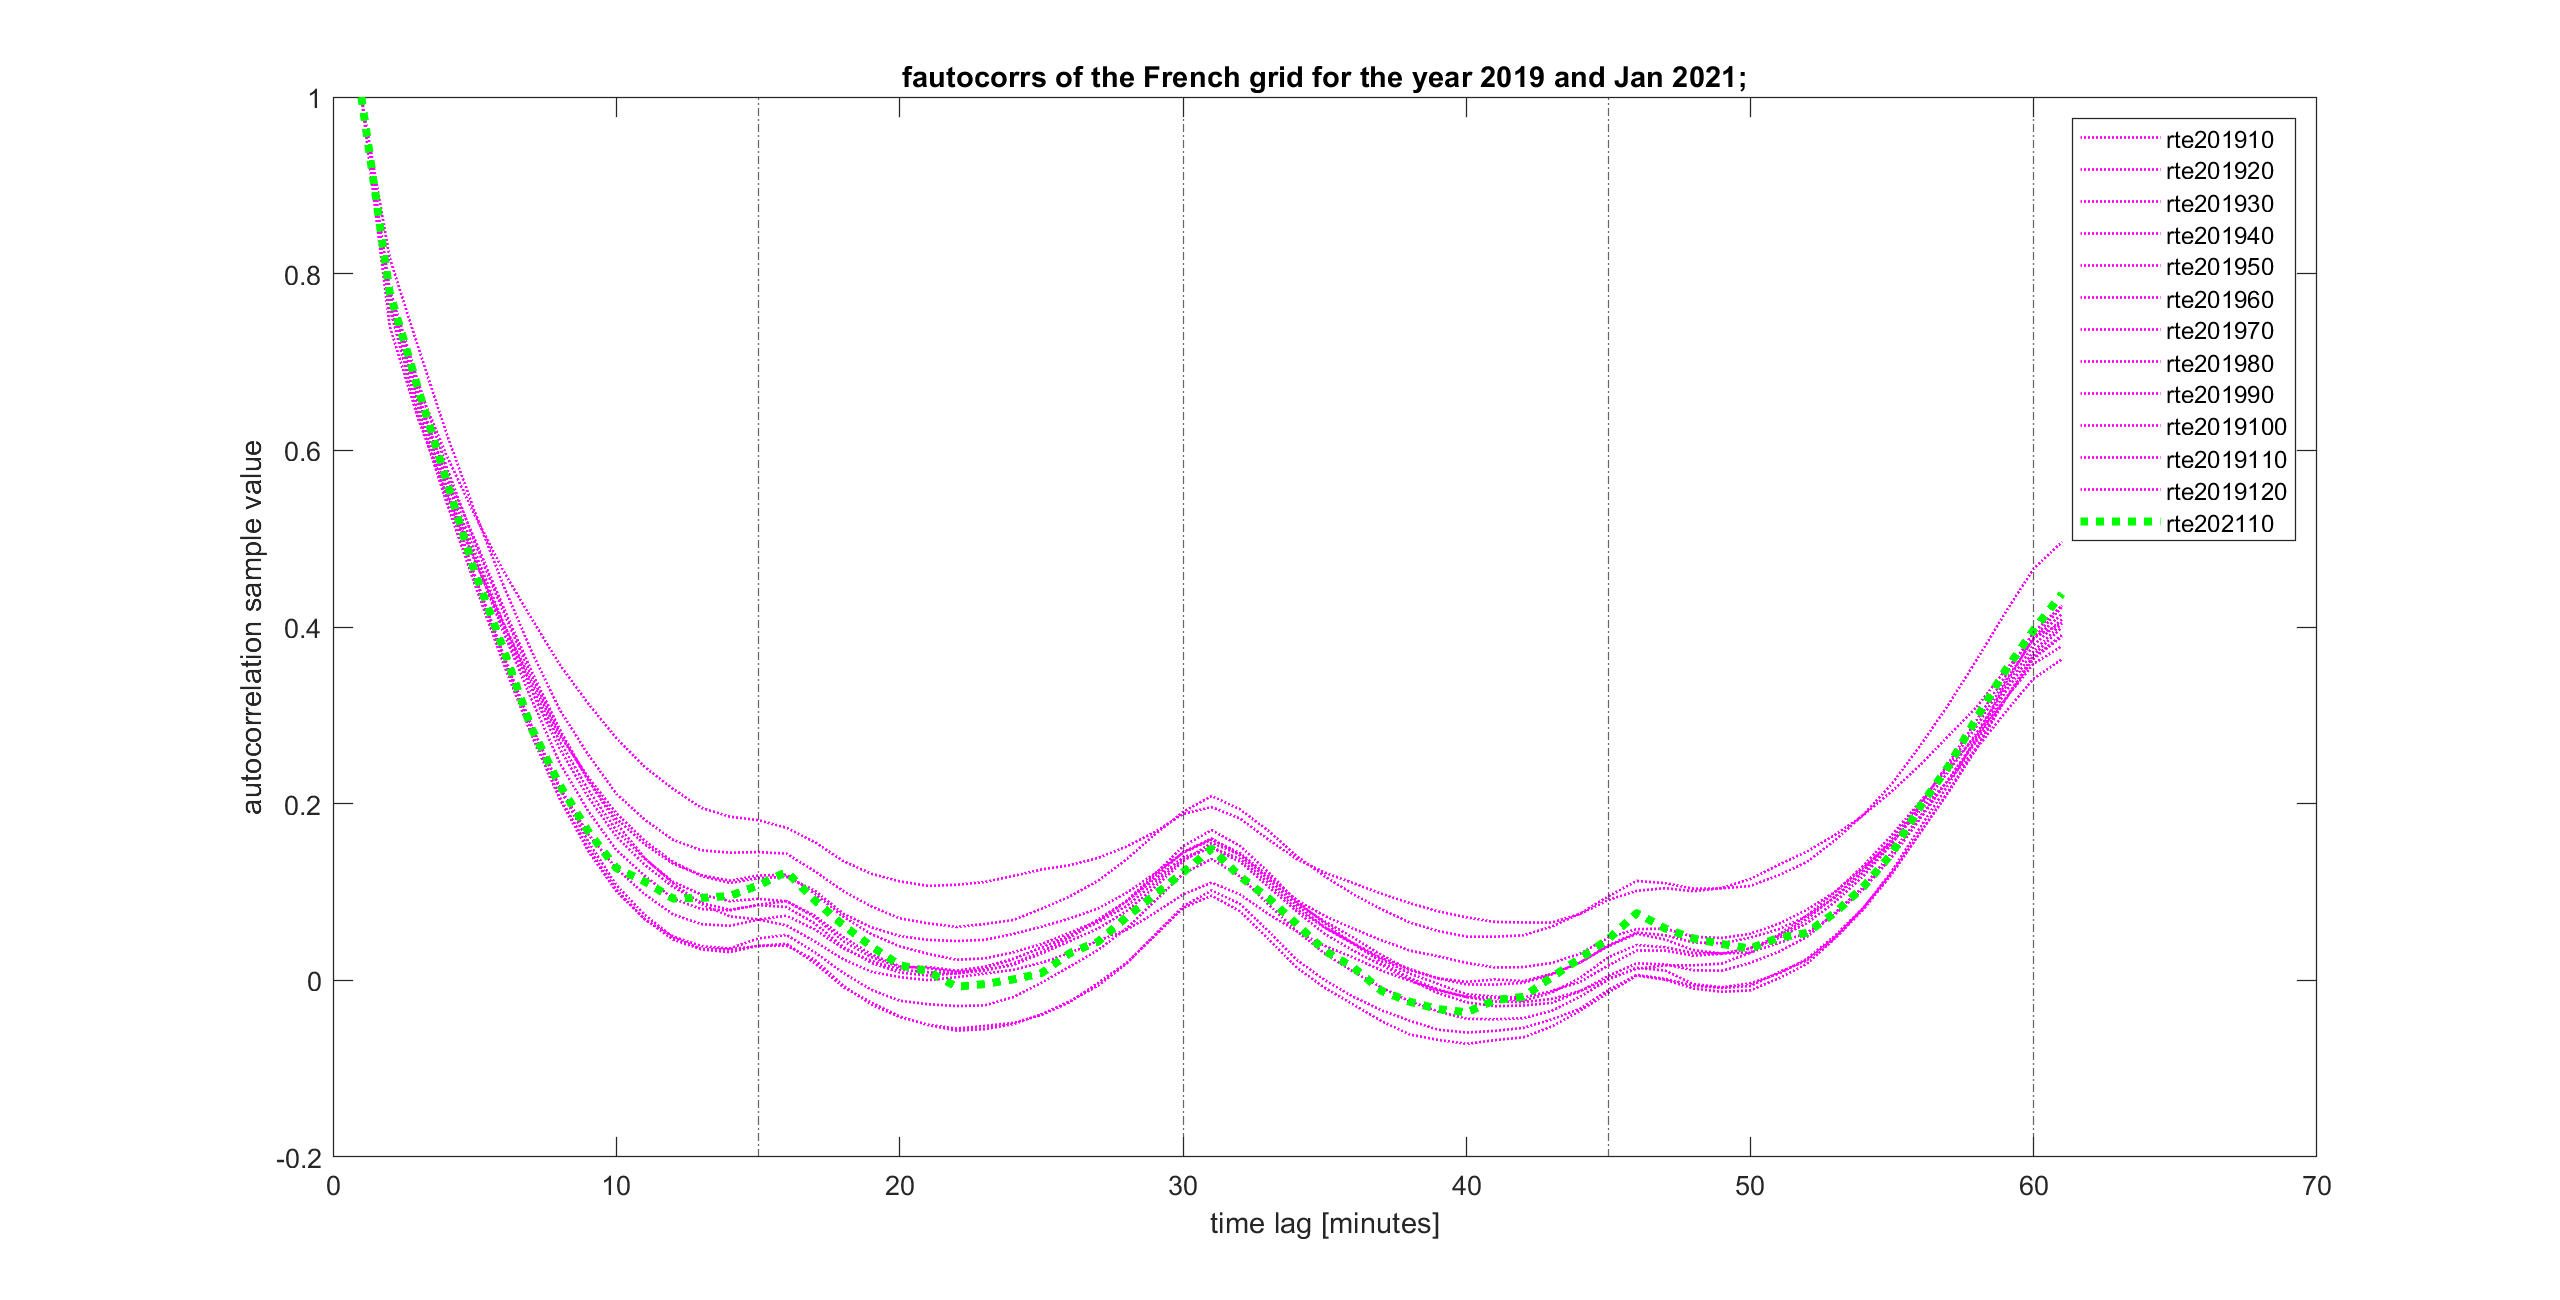
\includegraphics[scale=0.25]{../figures/autocorr/fautocorrs_rte_201901_to_201912_202101}
	\caption{Fixed Time Autocorrelation plots for the French Grid for twelve months of the year 2019 and January 2021. They present a fairly consistent picture of the grid's dynamics.}
\end{figure}

\begin{figure}[!ht]
	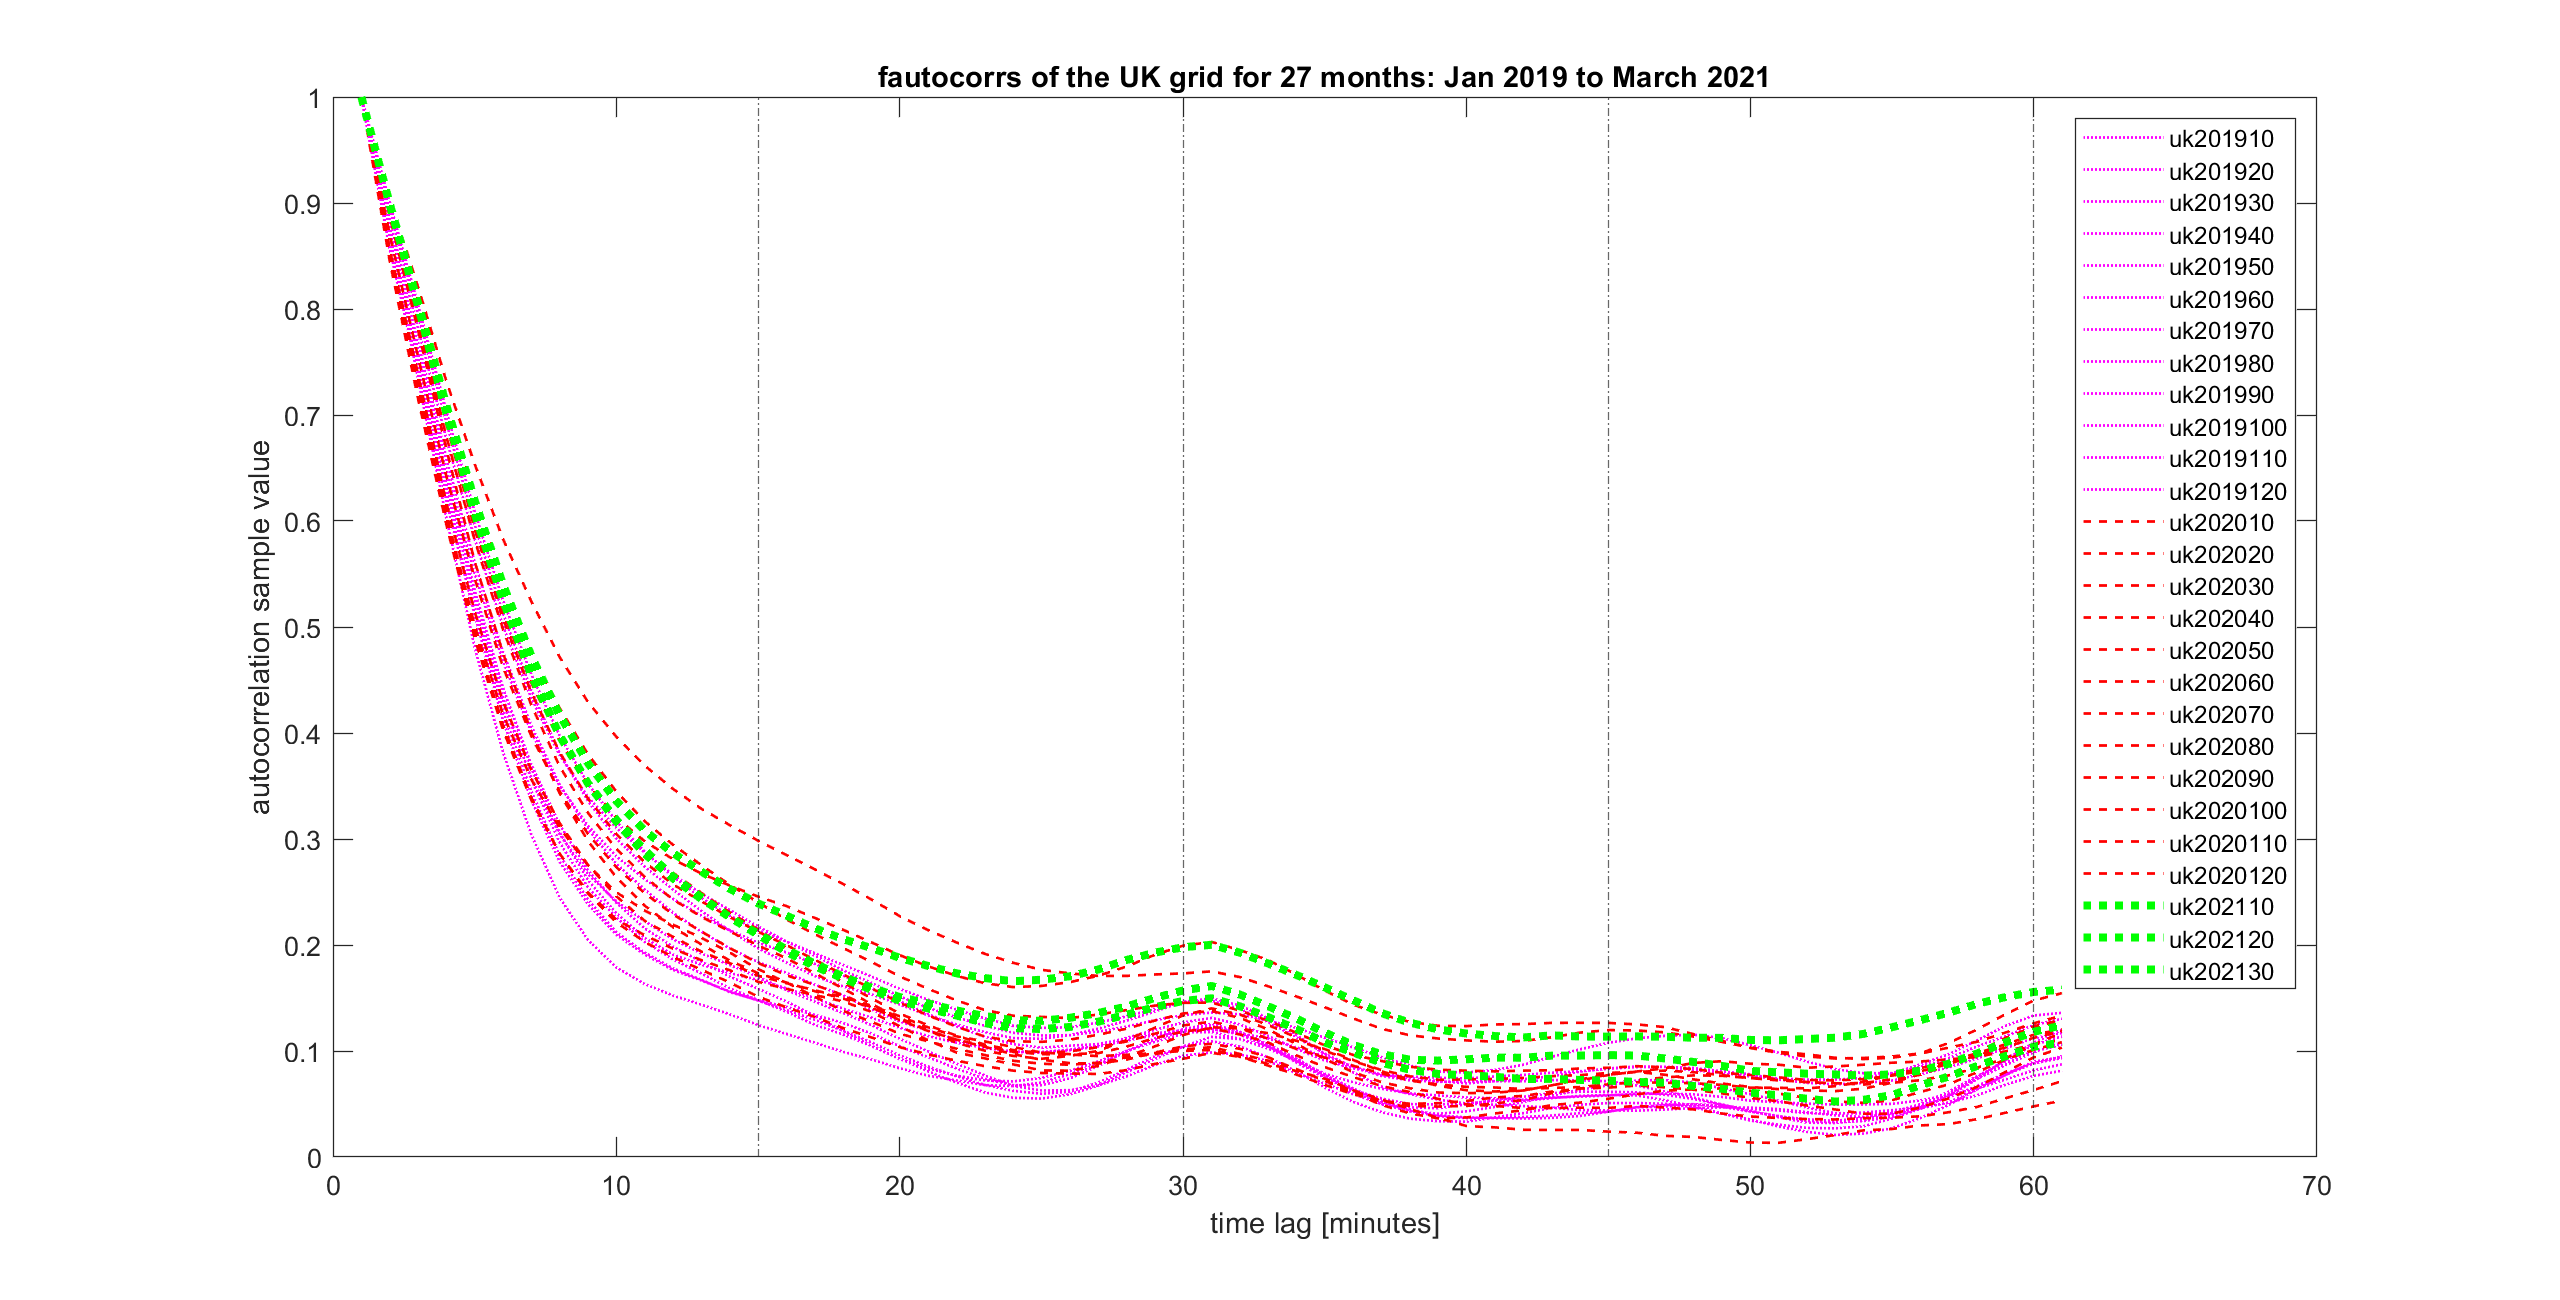
\includegraphics[scale=0.25]{../figures/autocorr/fautocorrs_uk_201901_to_202103_2}
	\caption{Fixed Time Autocorrelation plots for the Great Britain Grid for twenty seven continuous months, from January 2019 to March 2021. They present a fairly consistent picture of the grid's dynamics.}
\end{figure}

\begin{figure}[!ht]
	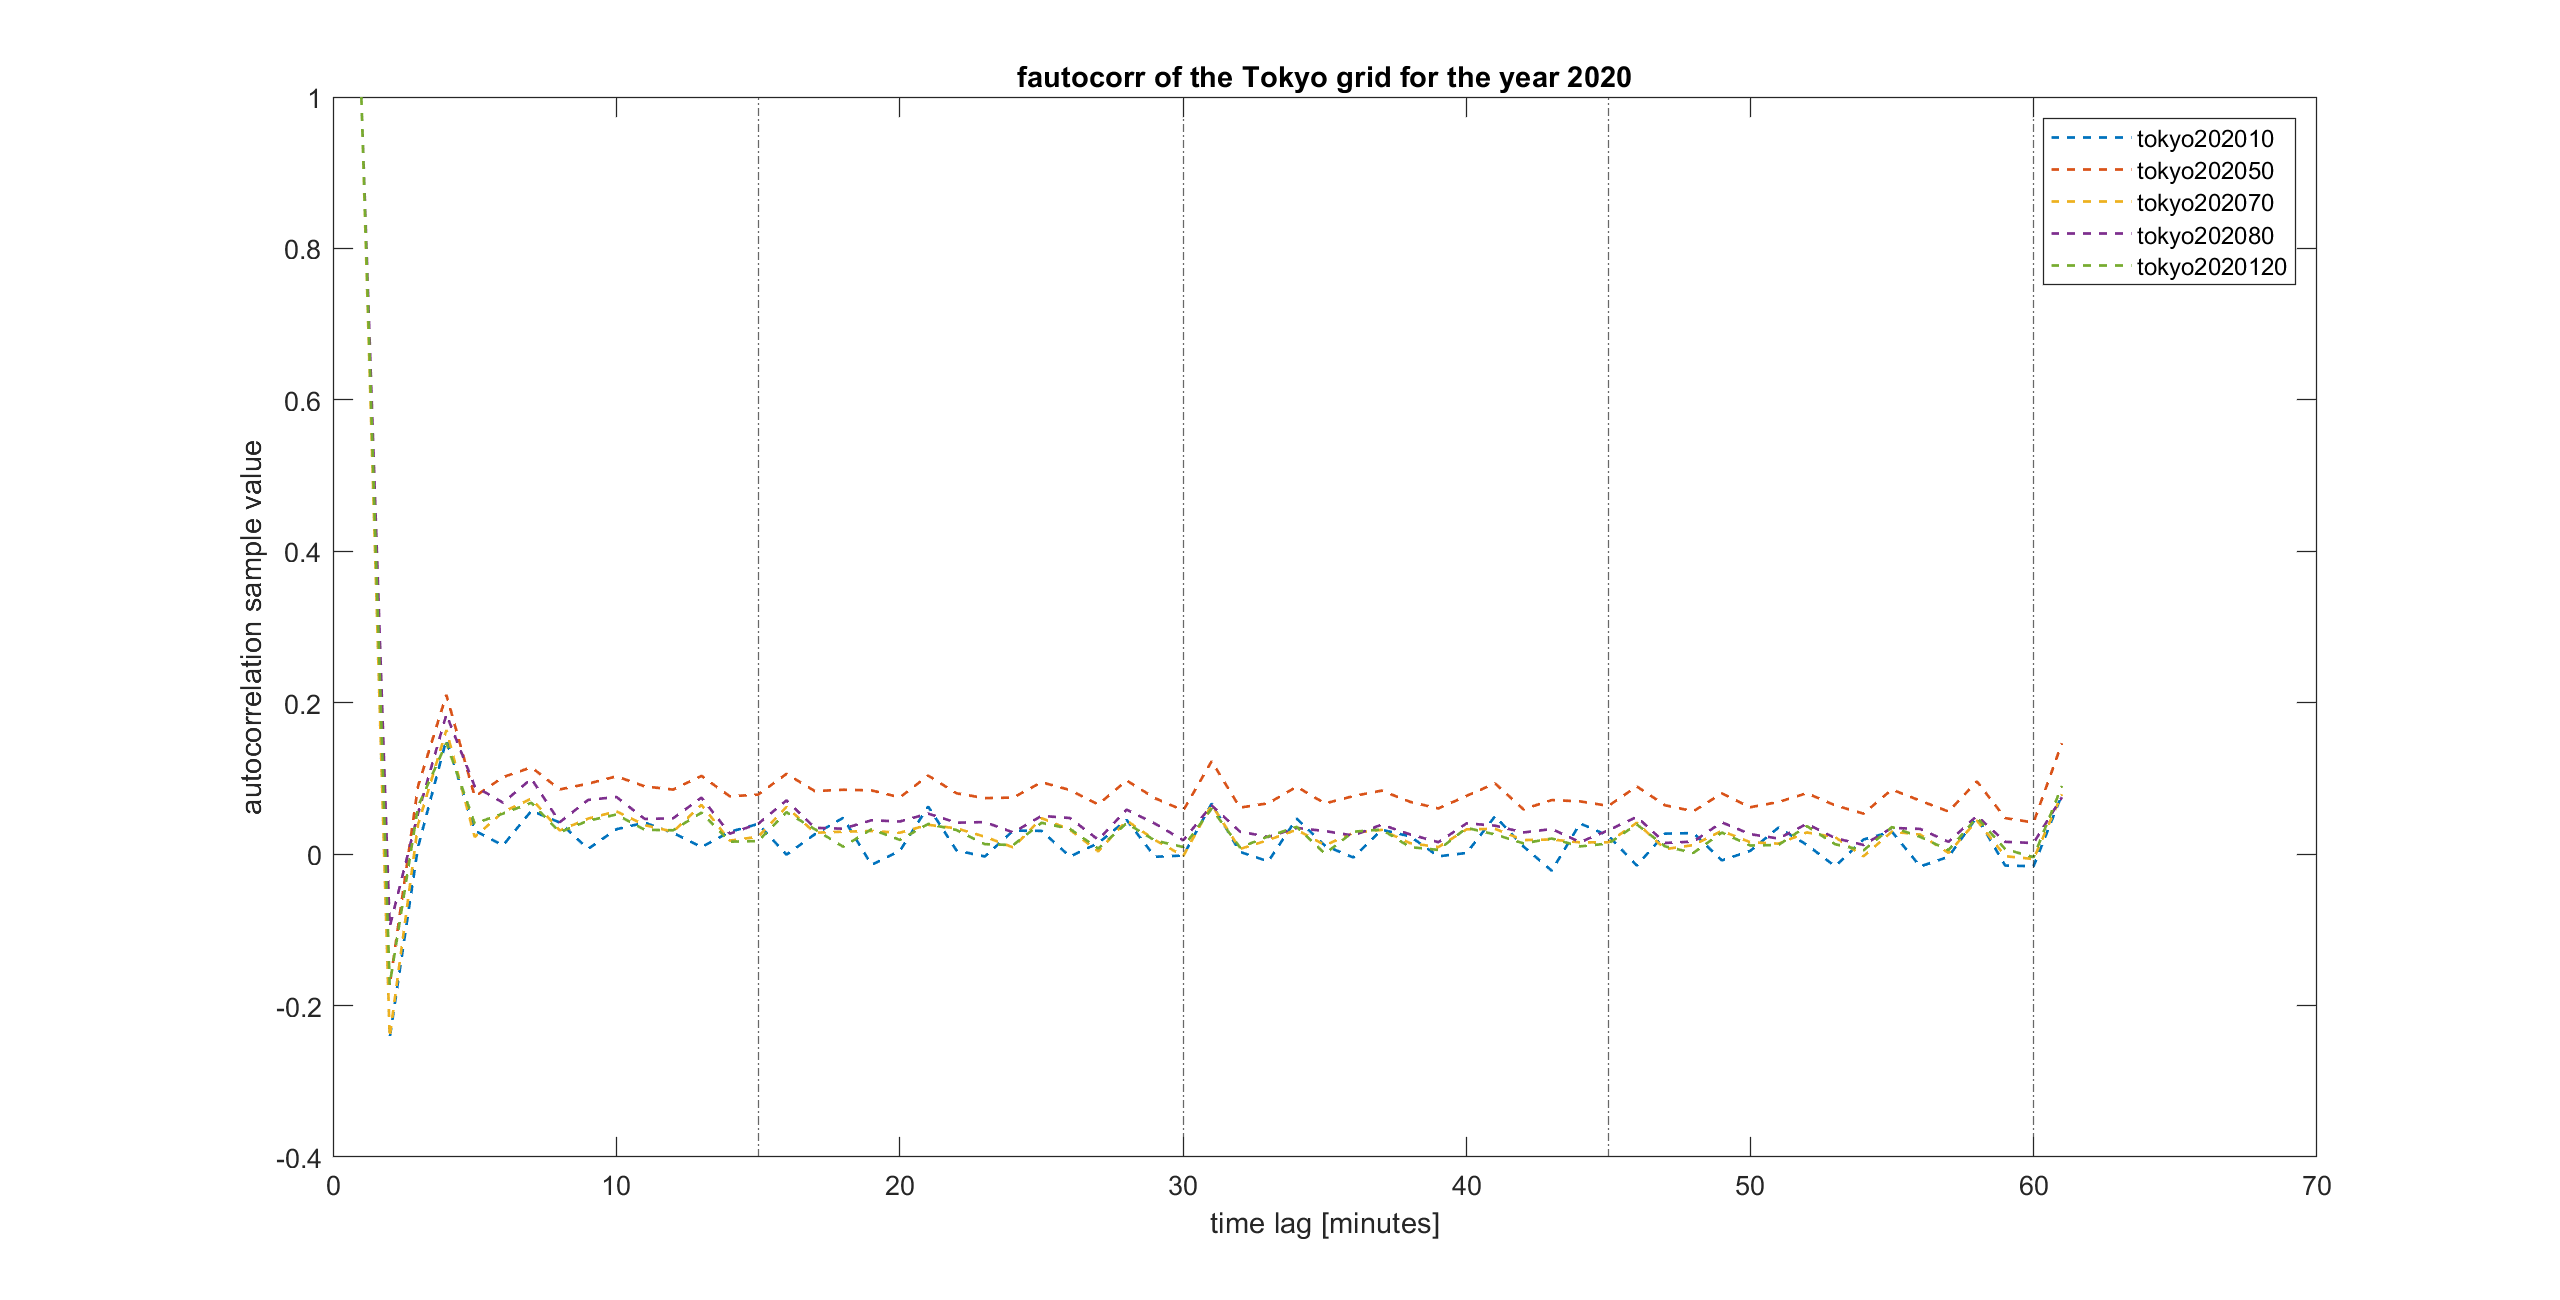
\includegraphics[scale=0.25]{../figures/autocorr/fautocorrs_tokyo_202001_to_202012}
	\caption{Fixed Time Autocorrelation plots for the Tokyo Grid for five non-continuous months of the year 2020: January, May, July, August and December. They present a fairly consistent picture of the grid's dynamics.}
\end{figure}

Data for six non-continuous days (07 April 2019, 03 July 2019, 08 August 2019, 14 December 2019, 01 February 2020 and 05 April 2020) for the Indian grid (NRLDC) was also compared in a similar fashion. Some of the days have also been marked with attributes to indicate notable demand-generation characteristics associated with the day, including: Day with minimum renewable generation, Day with maximum renewable generation contribution (07 April 2019), Day with minimum solar power contribution (08 August 2019), Day with lowest power demand (14 December 2019) and Day with lowest renewable generation contribution (01 February 2020). The plots were inconsistent and therefore a day's worth of data could be considered insufficient to average-out all the dynamic differences in a grid's statistical signature.

\begin{figure}[!ht]
	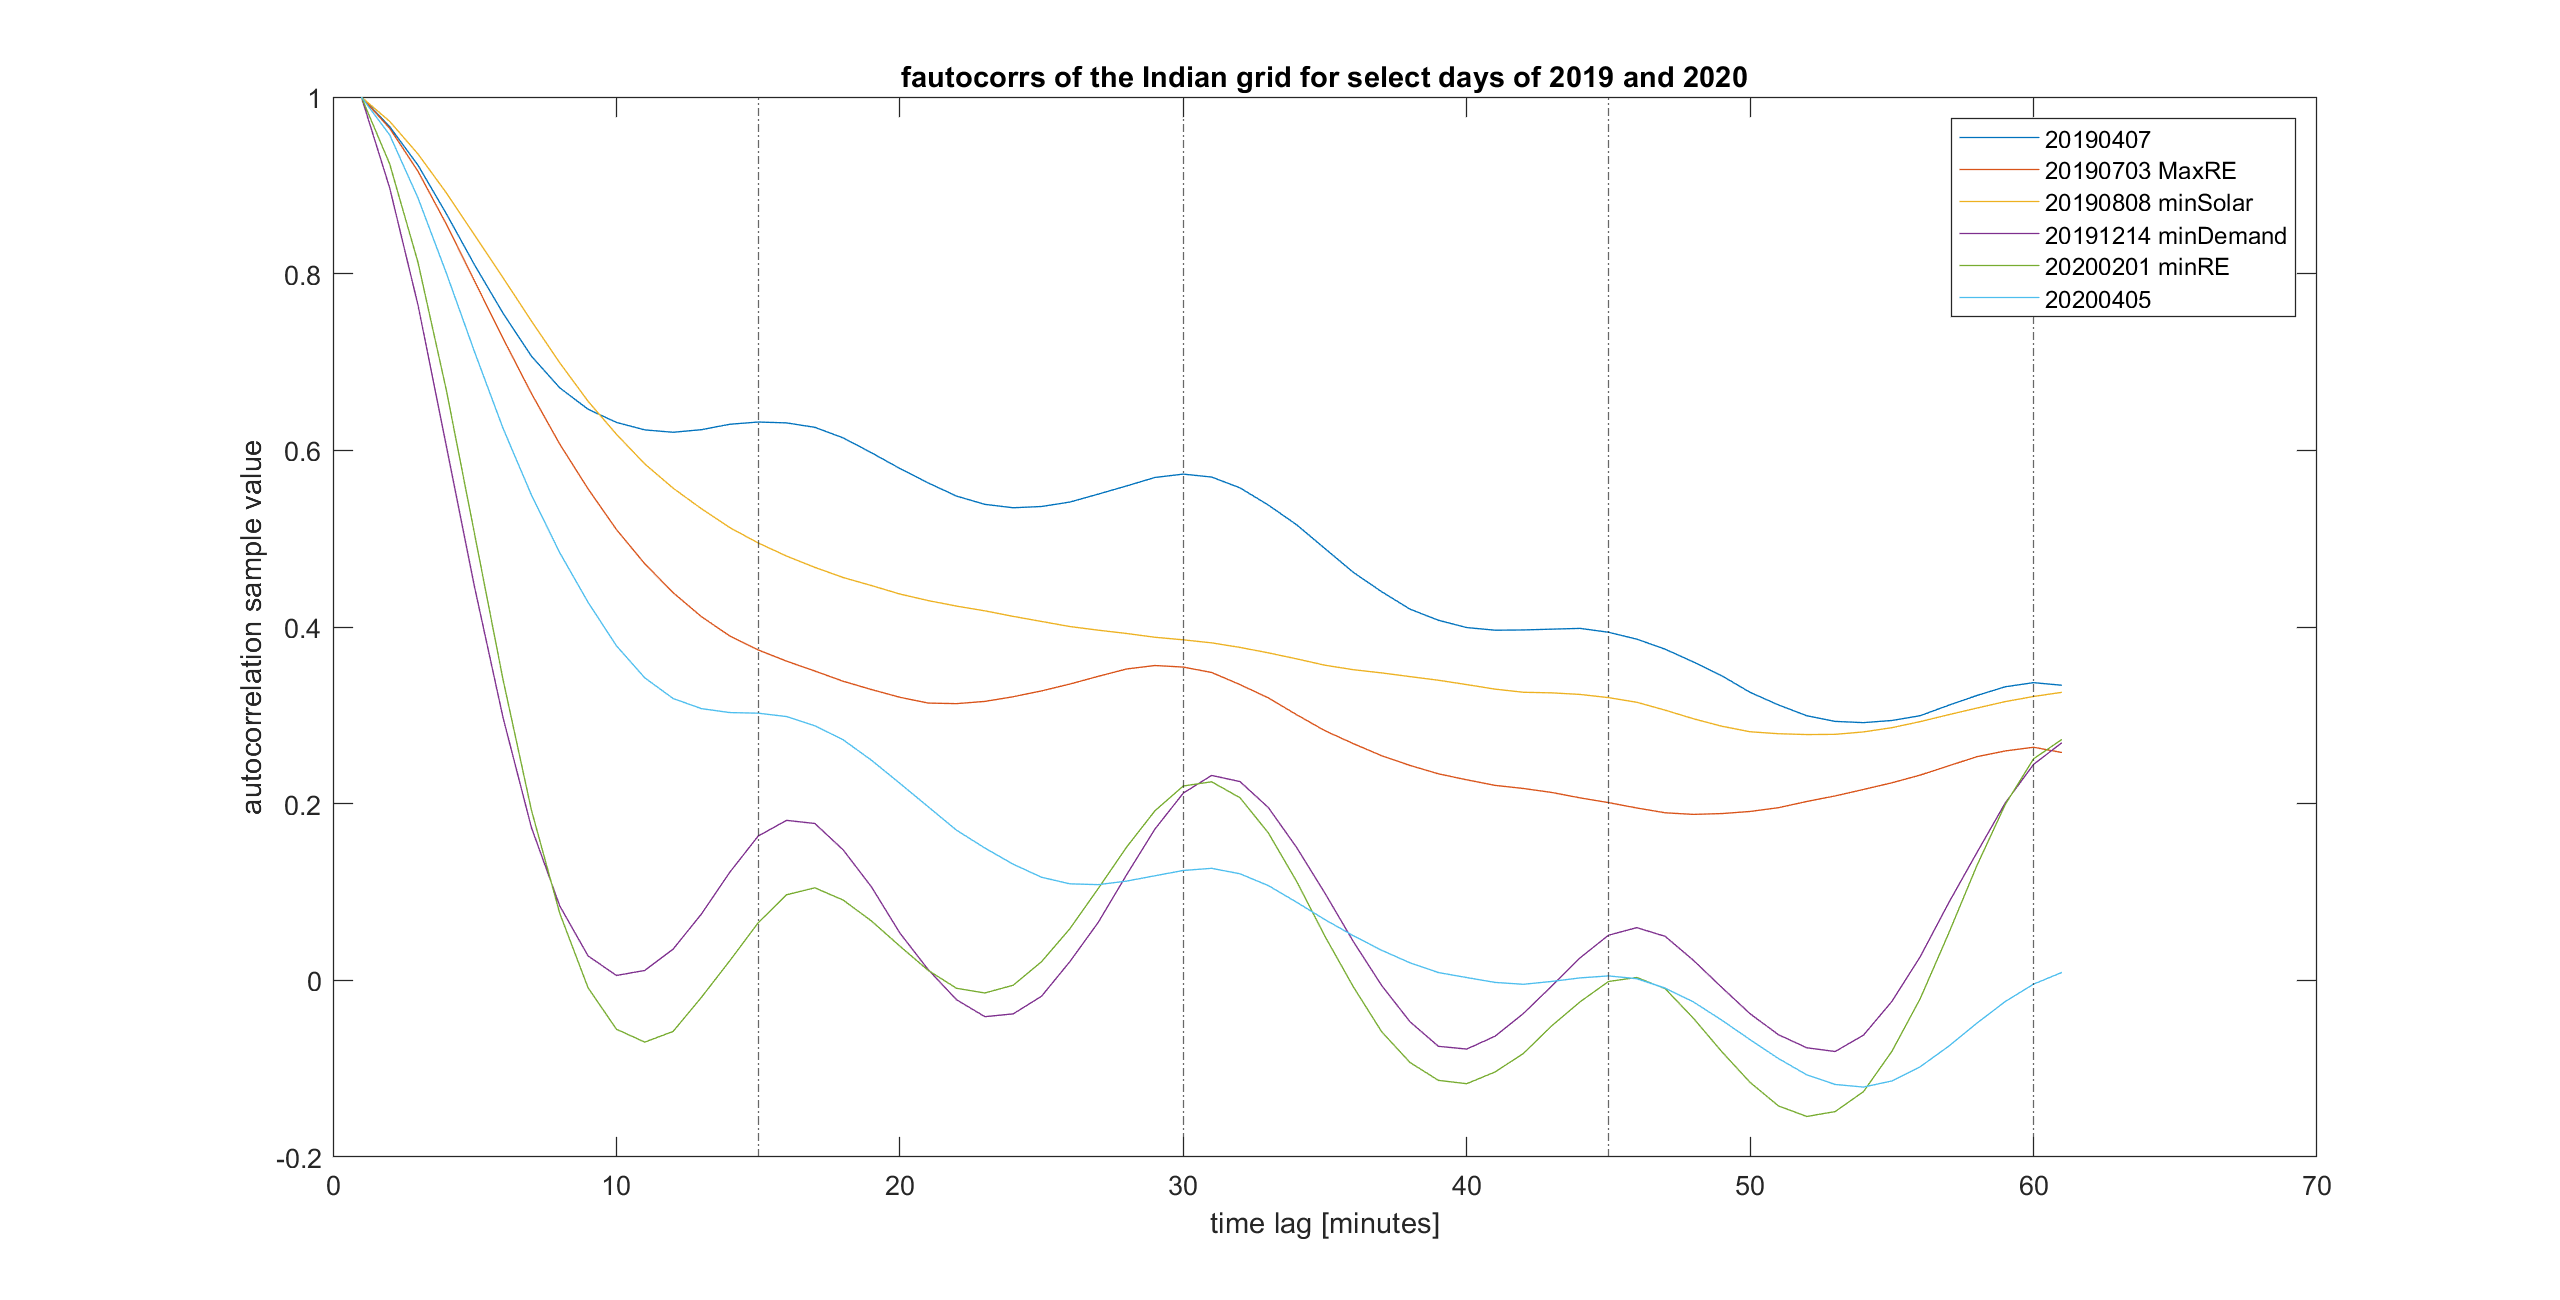
\includegraphics[scale=0.25]{../figures/autocorr/fautocorrs_nrldc_201904_to_202004}
	\caption{Fixed Time Autocorrelation Plots for Six non-continuous days of the Indian Grid: 07 April 2019, 03 July 2019, 08 August 2019, 14 December 2019, 01 February 2020 and 05 April 2020. Some of the days have also been marked with attributes with notable demand-generation characteristics associated with the day.}
\end{figure}

\begin{figure}[htp]
	\centering
	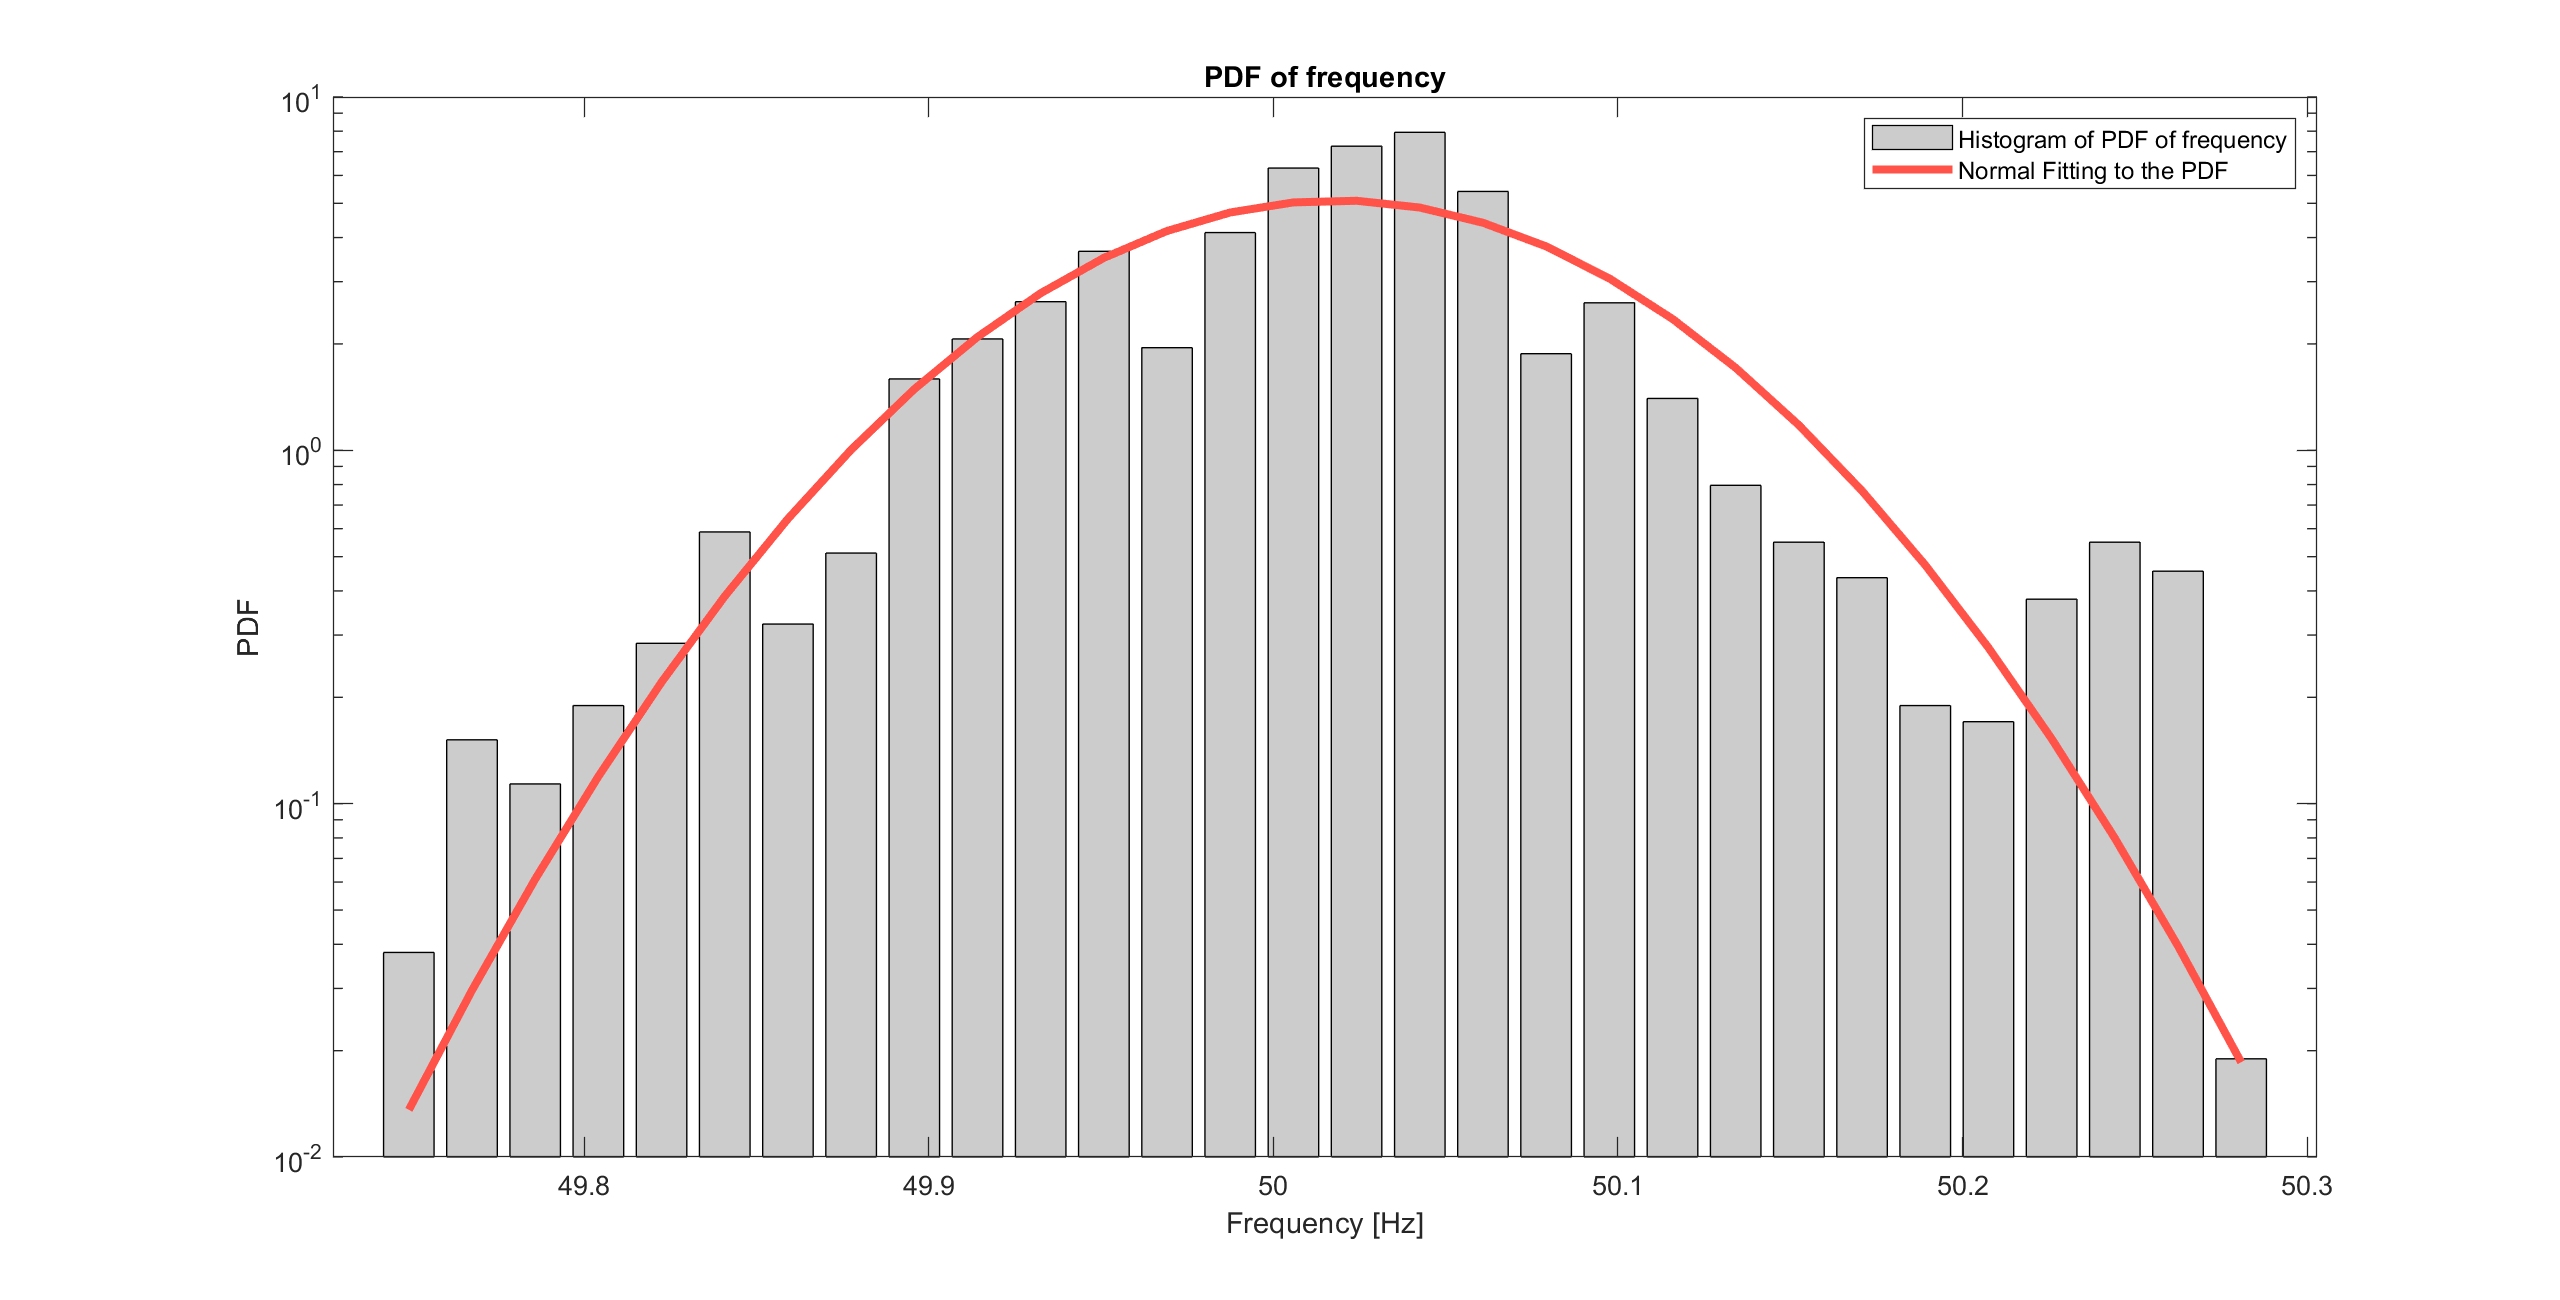
\includegraphics[width=.45\textwidth]{../figures/pdf/nrldc/pdf_frequency_nrldc_01}\quad
	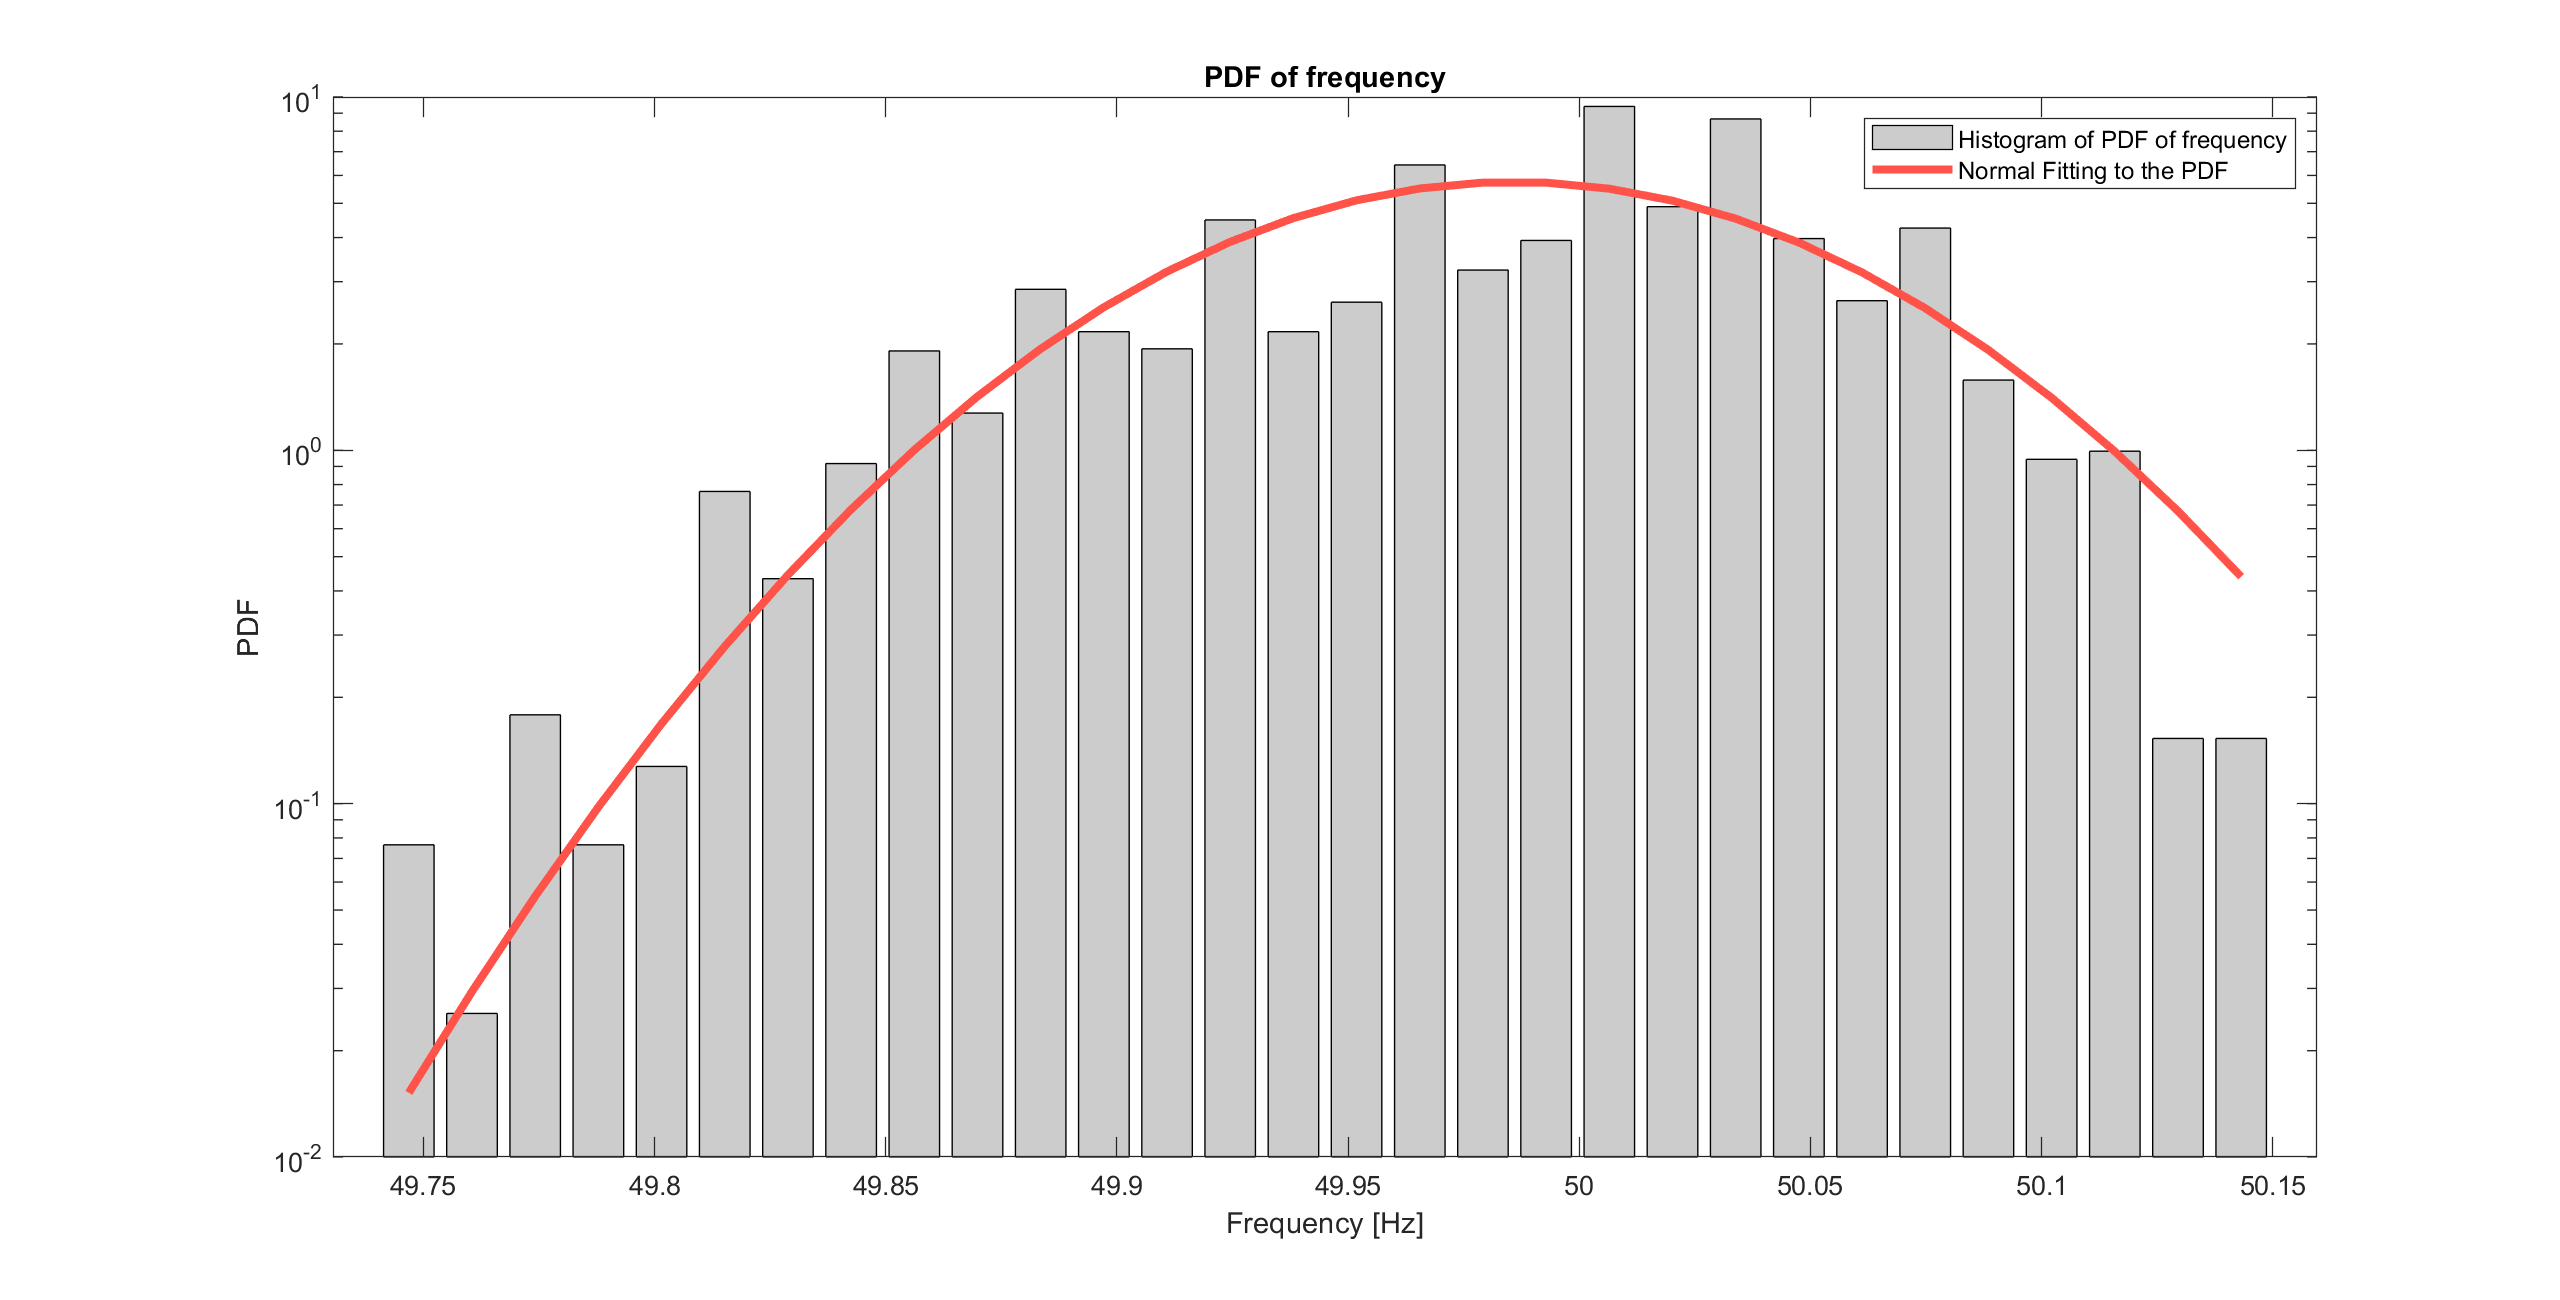
\includegraphics[width=.45\textwidth]{../figures/pdf/nrldc/pdf_frequency_nrldc_02}
	
	\medskip
	
	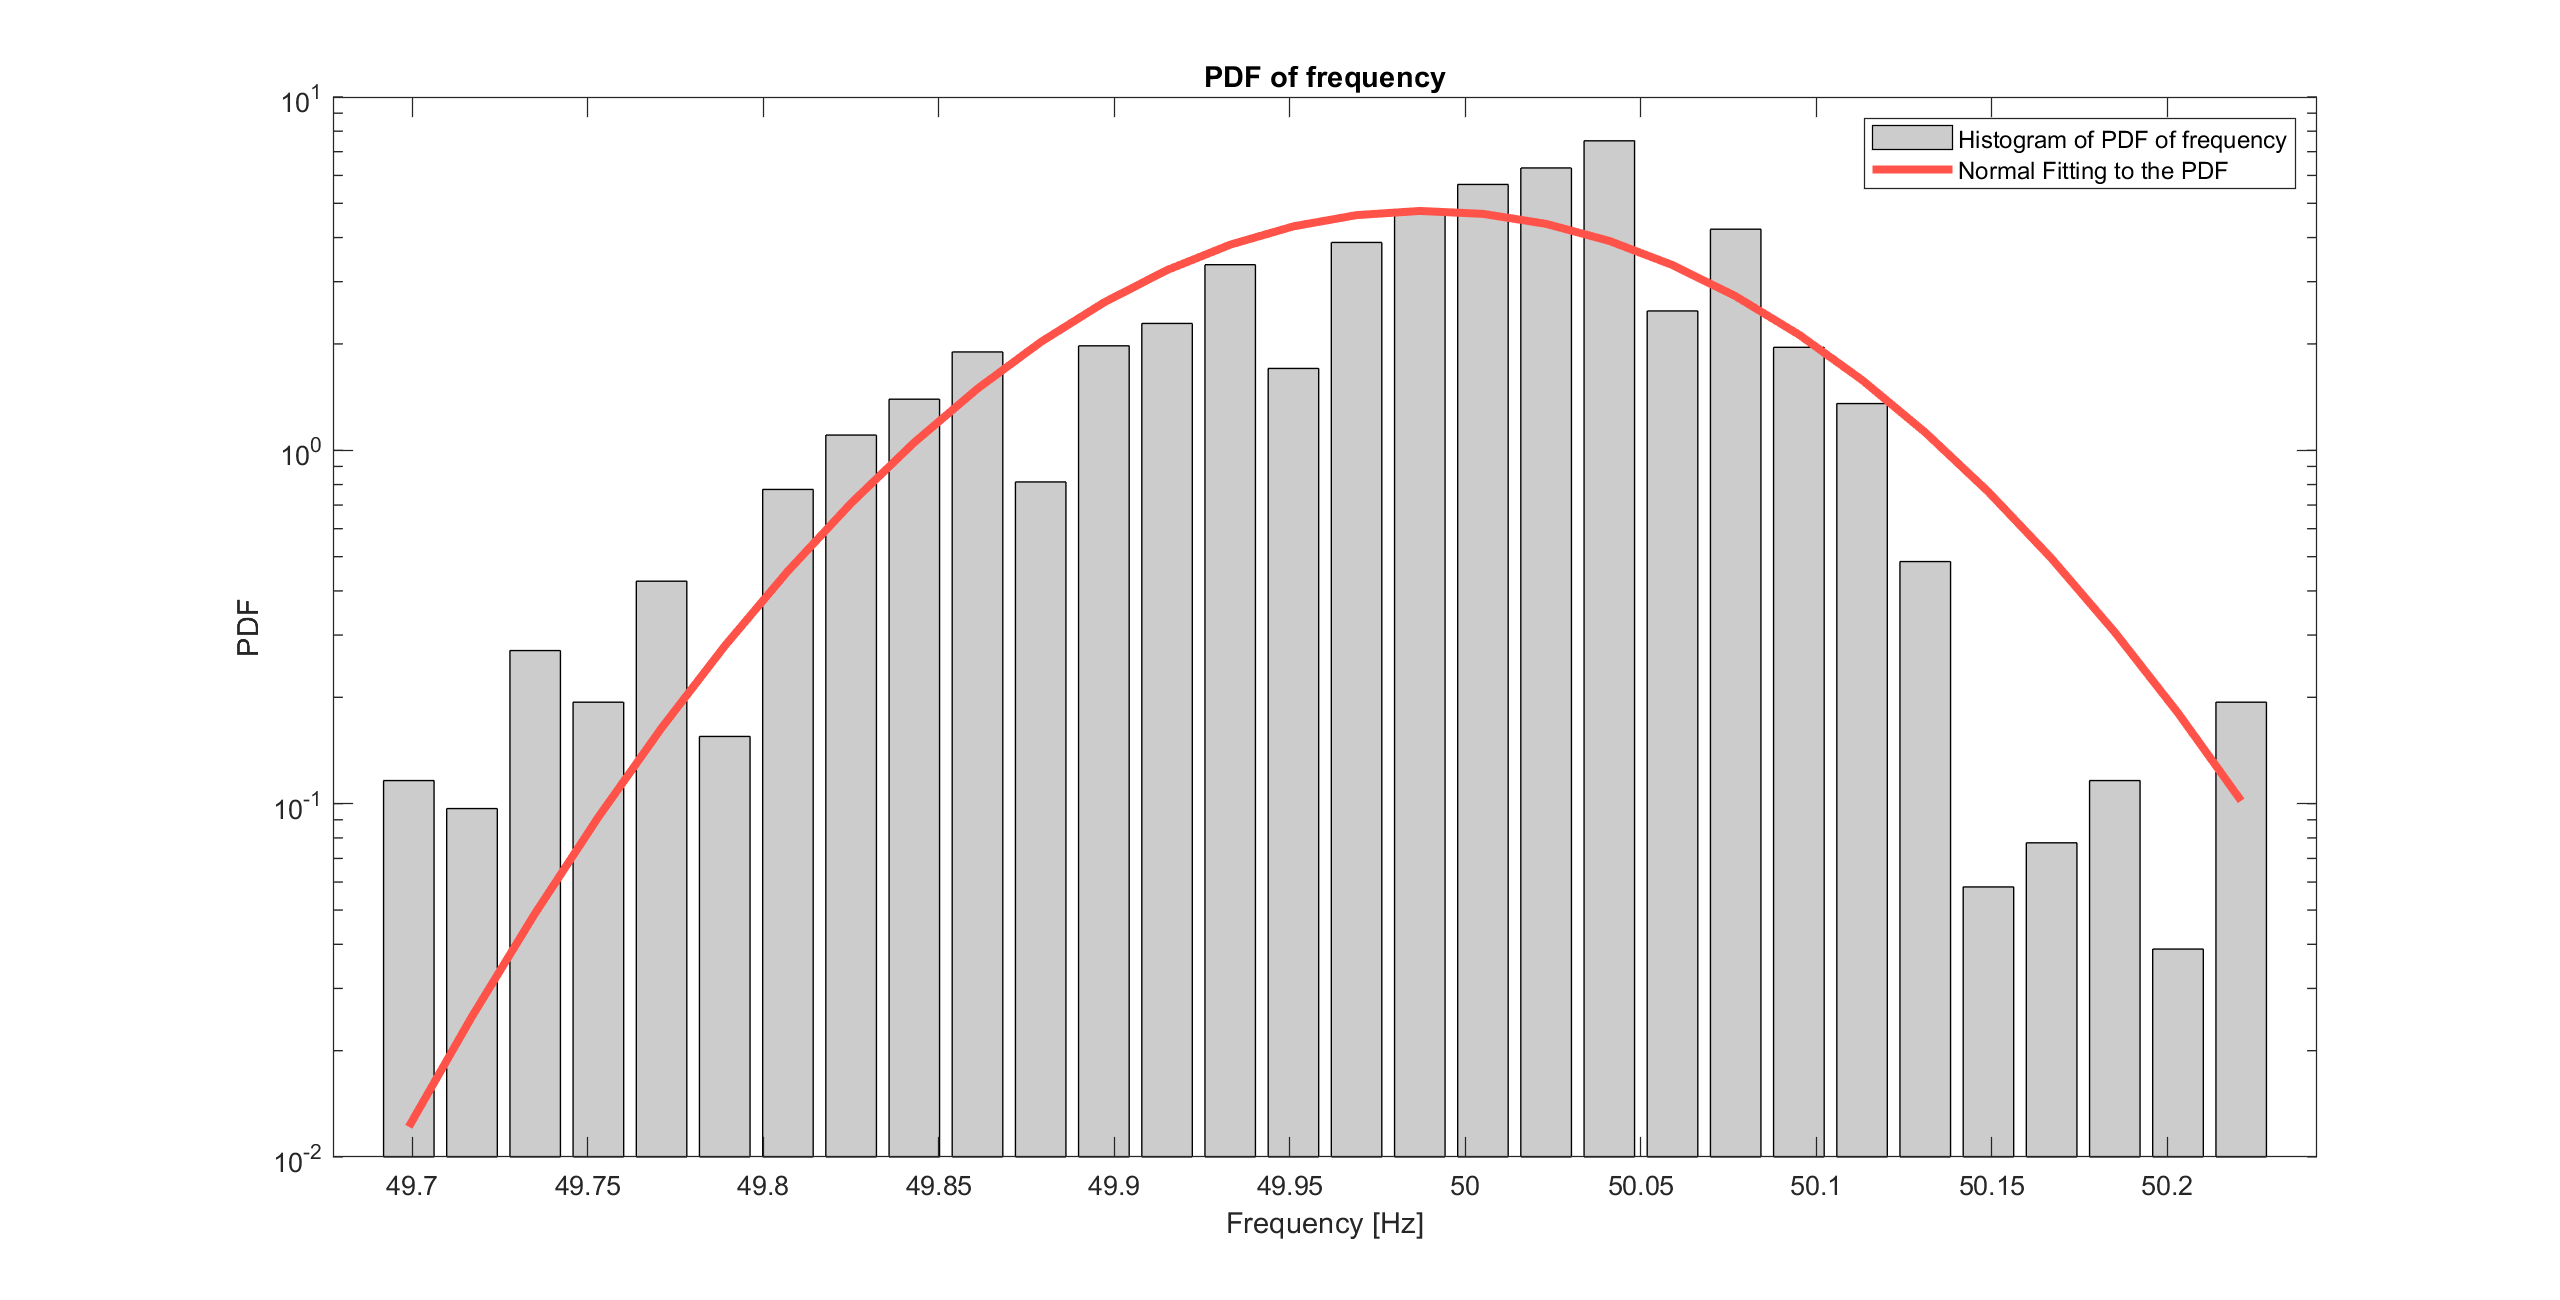
\includegraphics[width=.45\textwidth]{../figures/pdf/nrldc/pdf_frequency_nrldc_03}\quad
	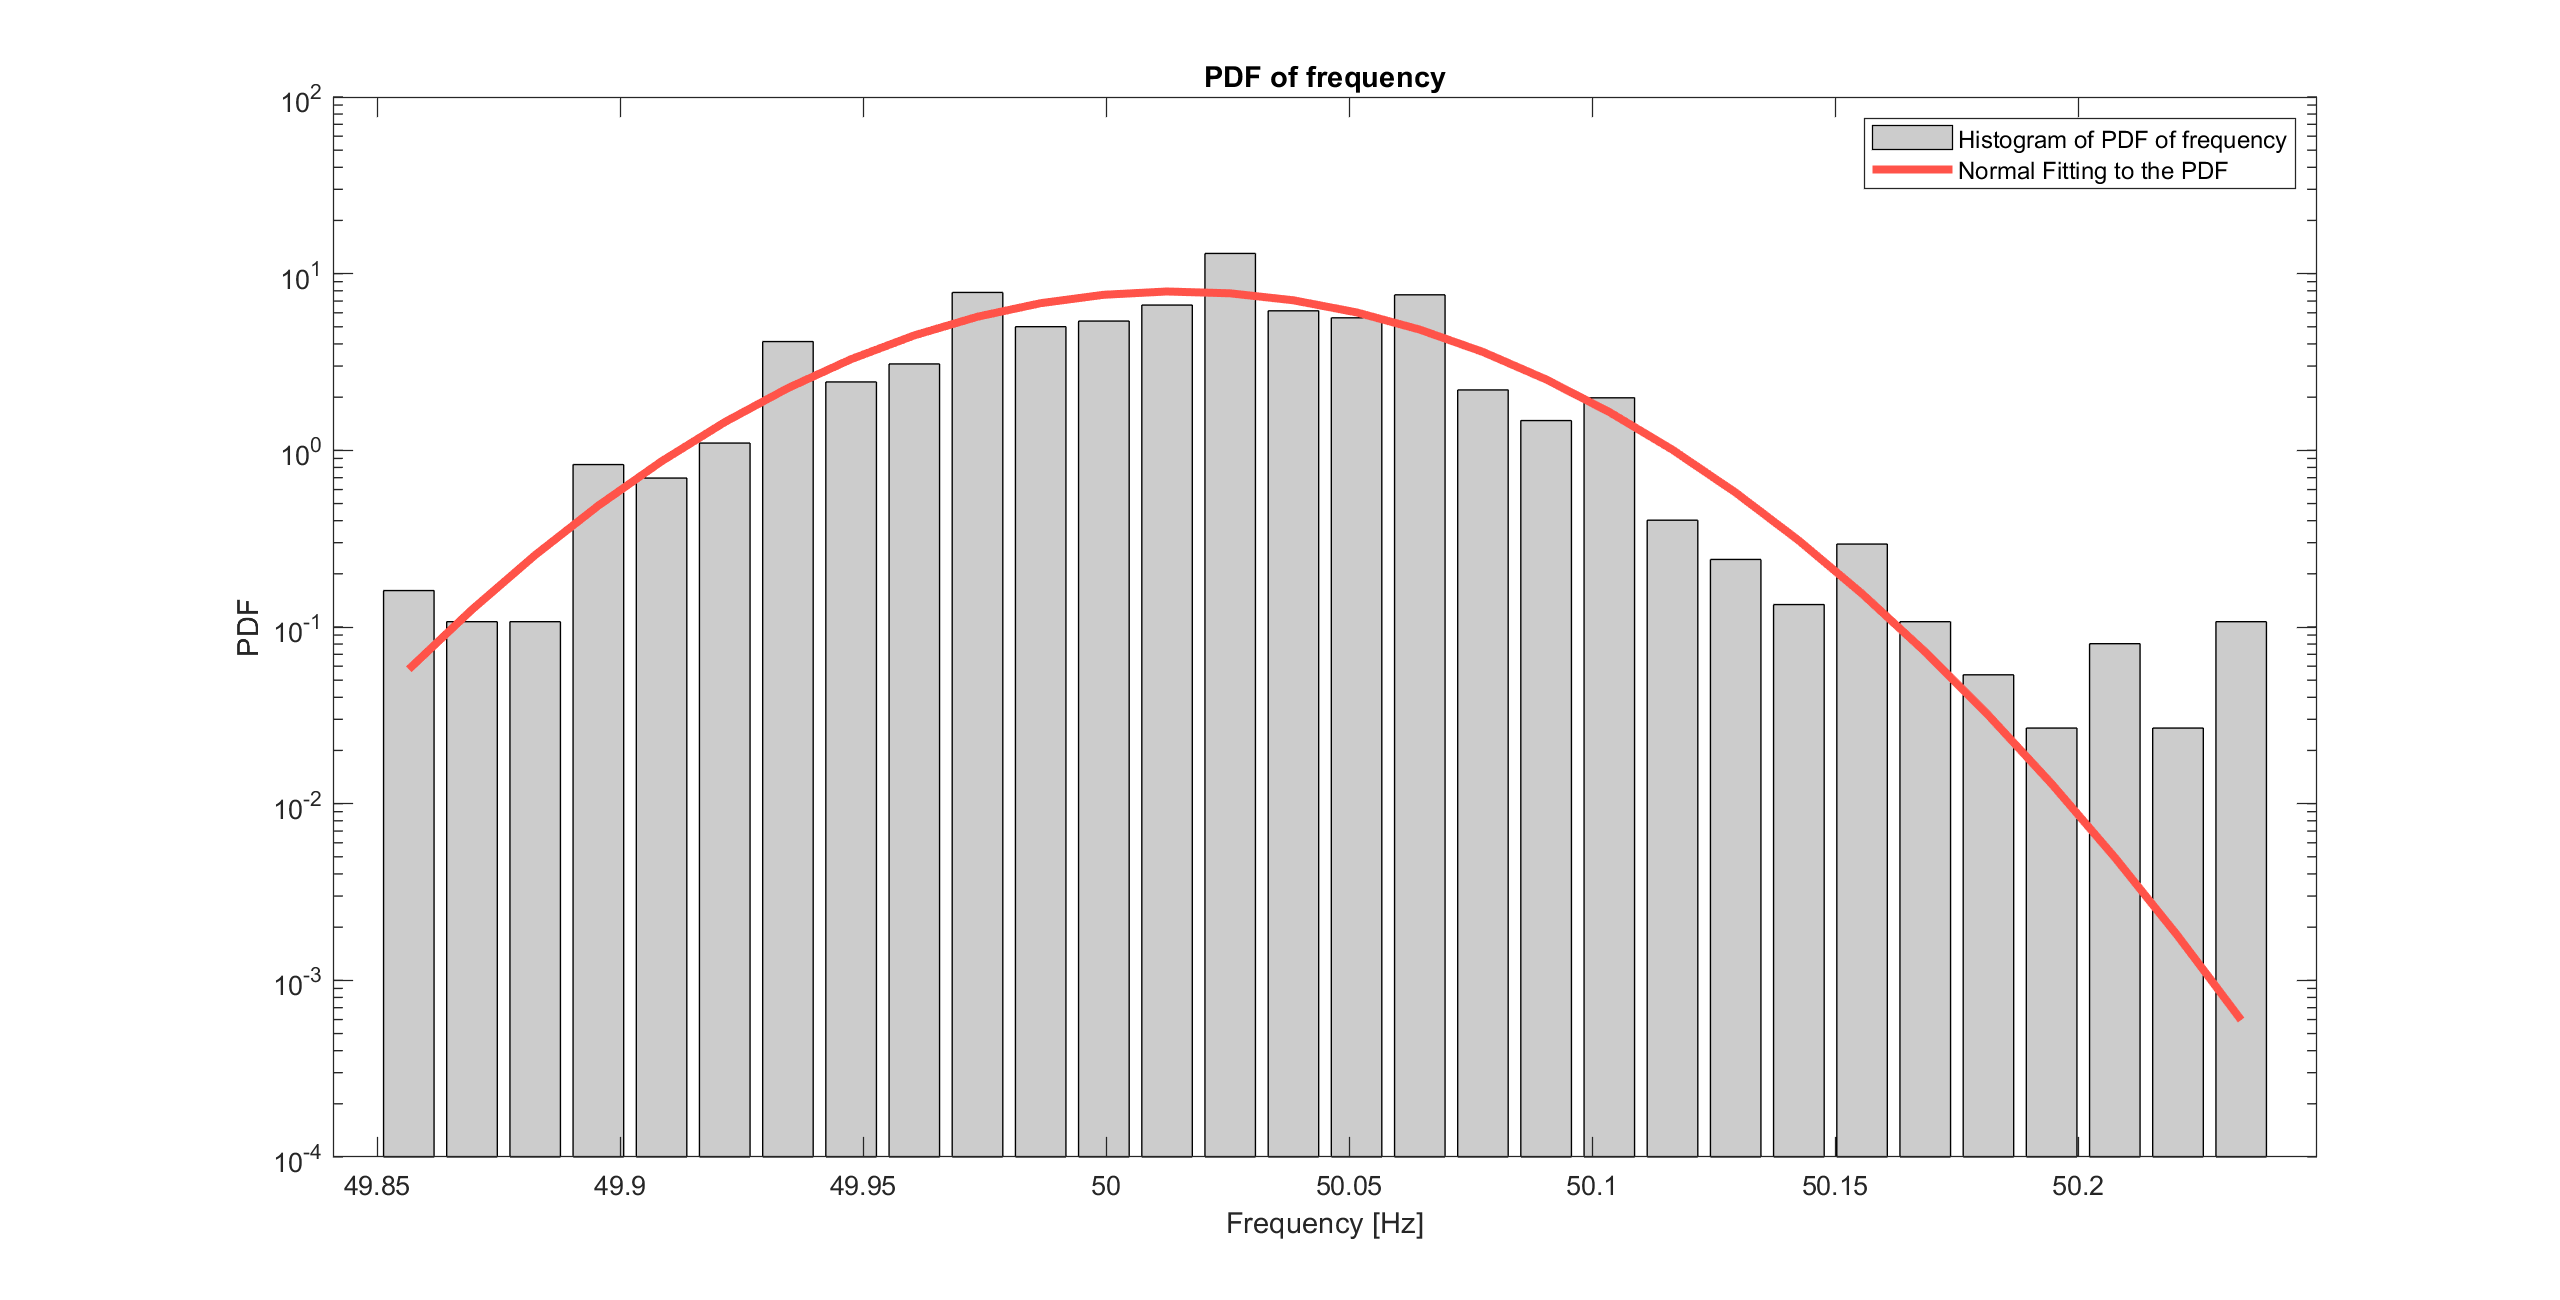
\includegraphics[width=.45\textwidth]{../figures/pdf/nrldc/pdf_frequency_nrldc_04}
	
	\medskip
	
	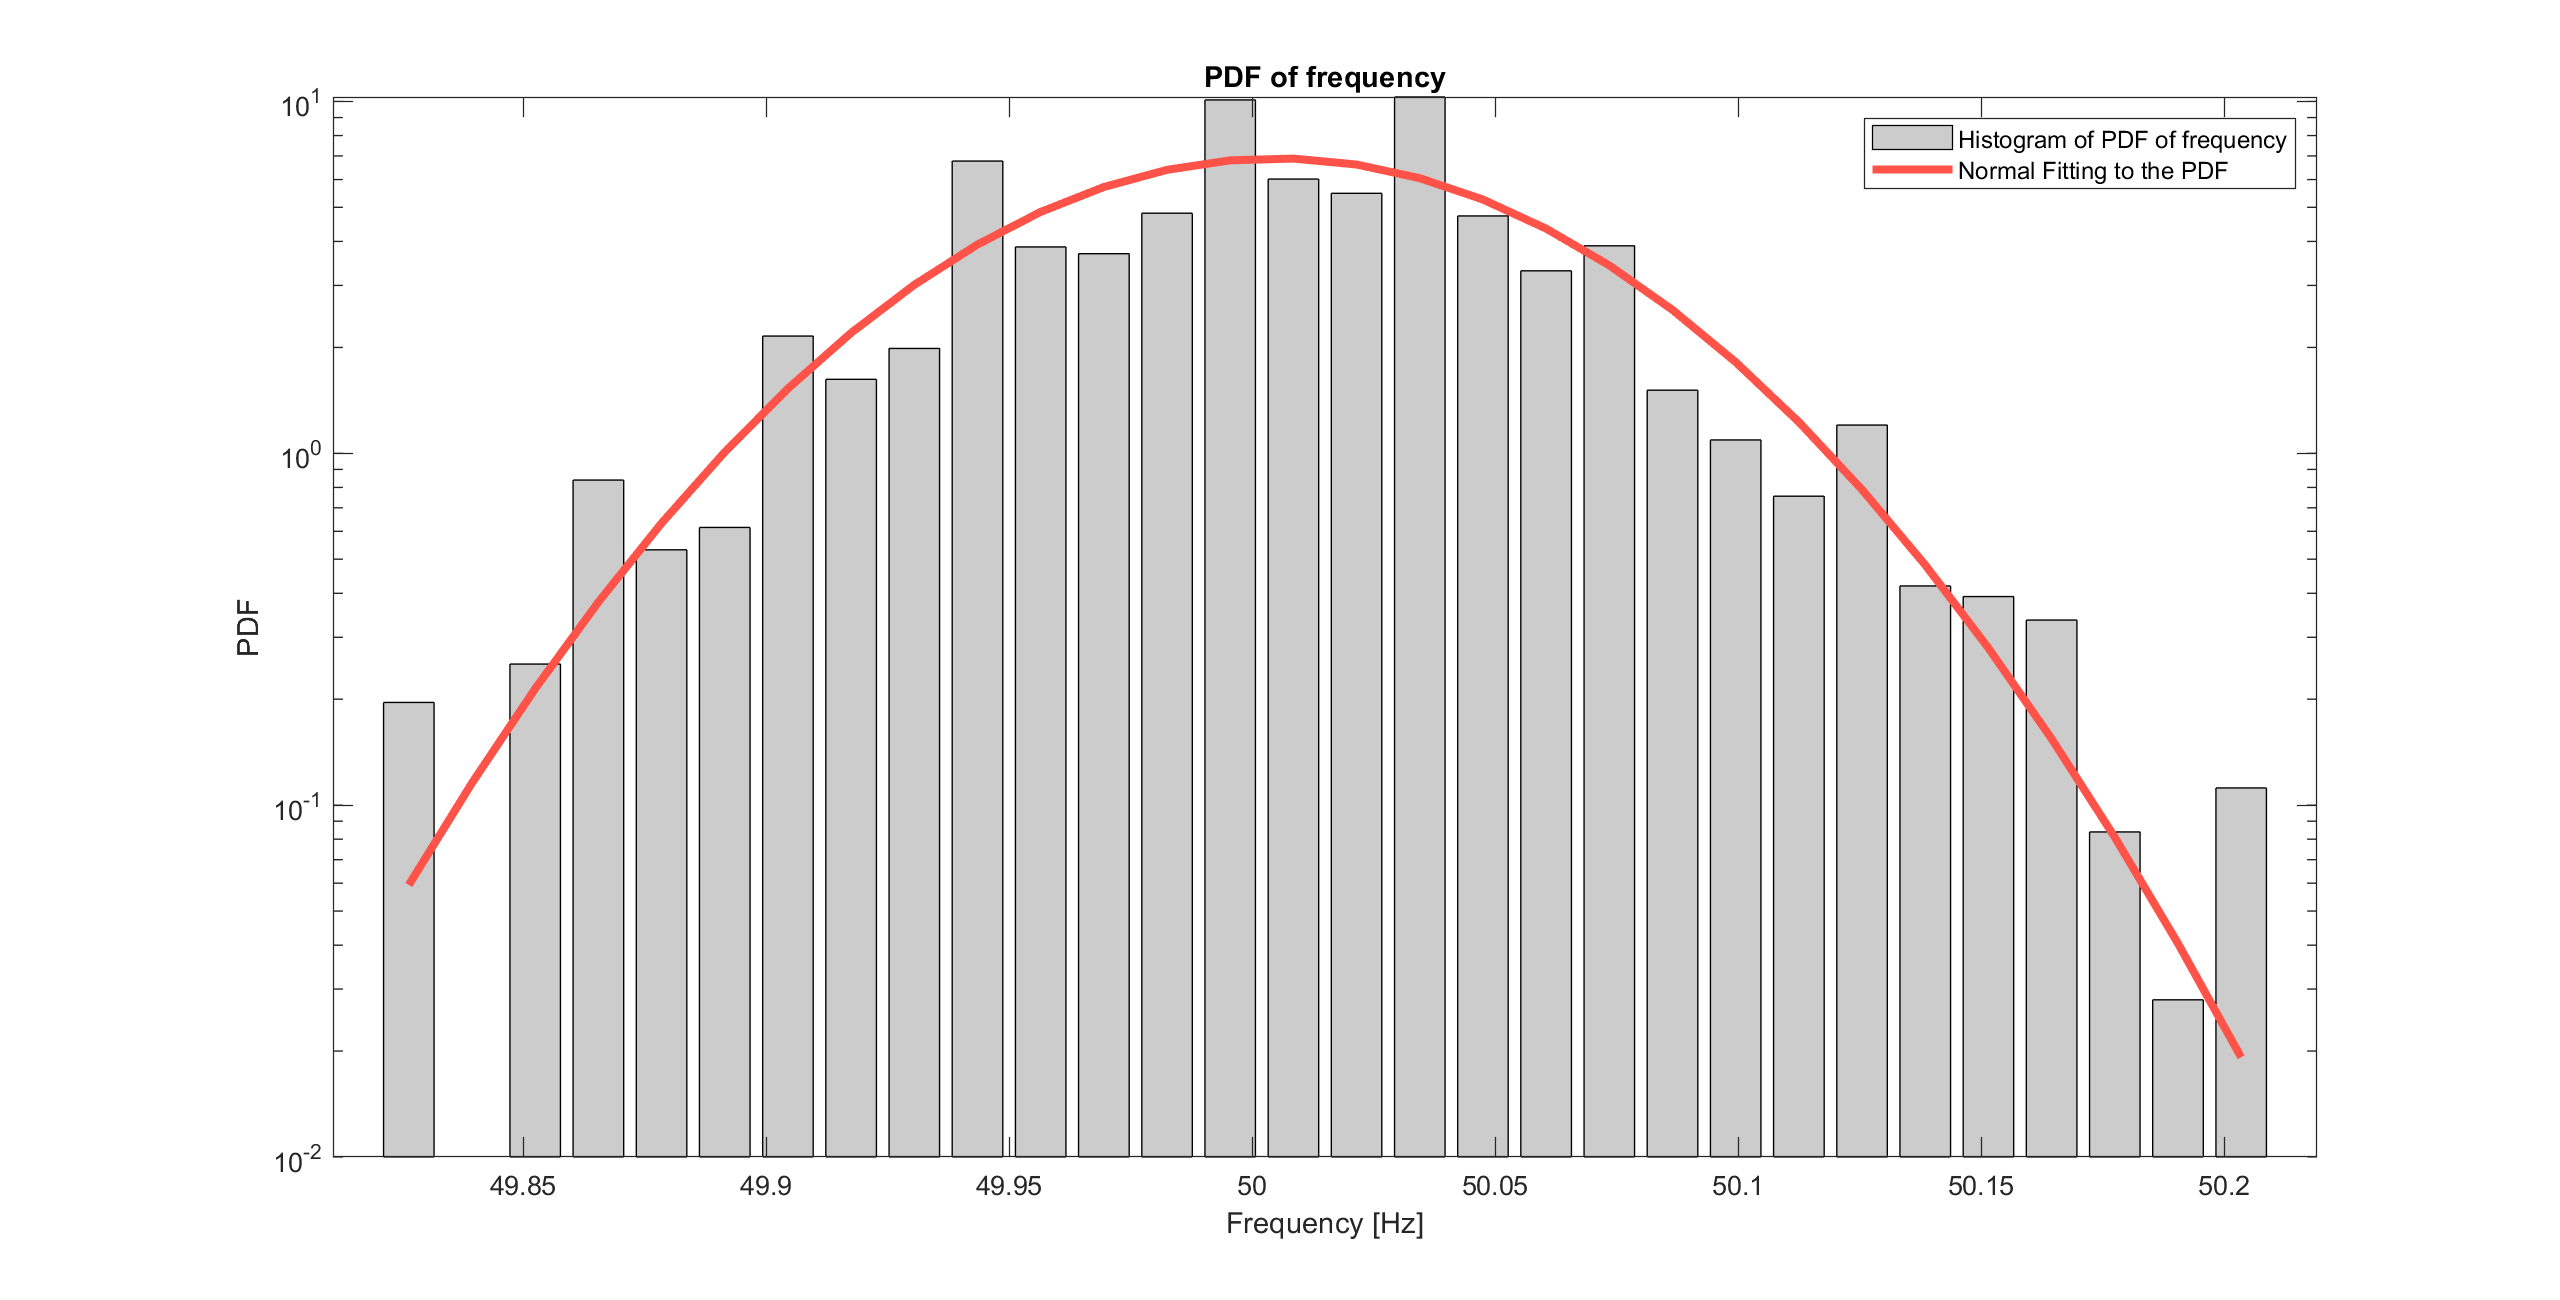
\includegraphics[width=.45\textwidth]{../figures/pdf/nrldc/pdf_frequency_nrldc_05}\quad
	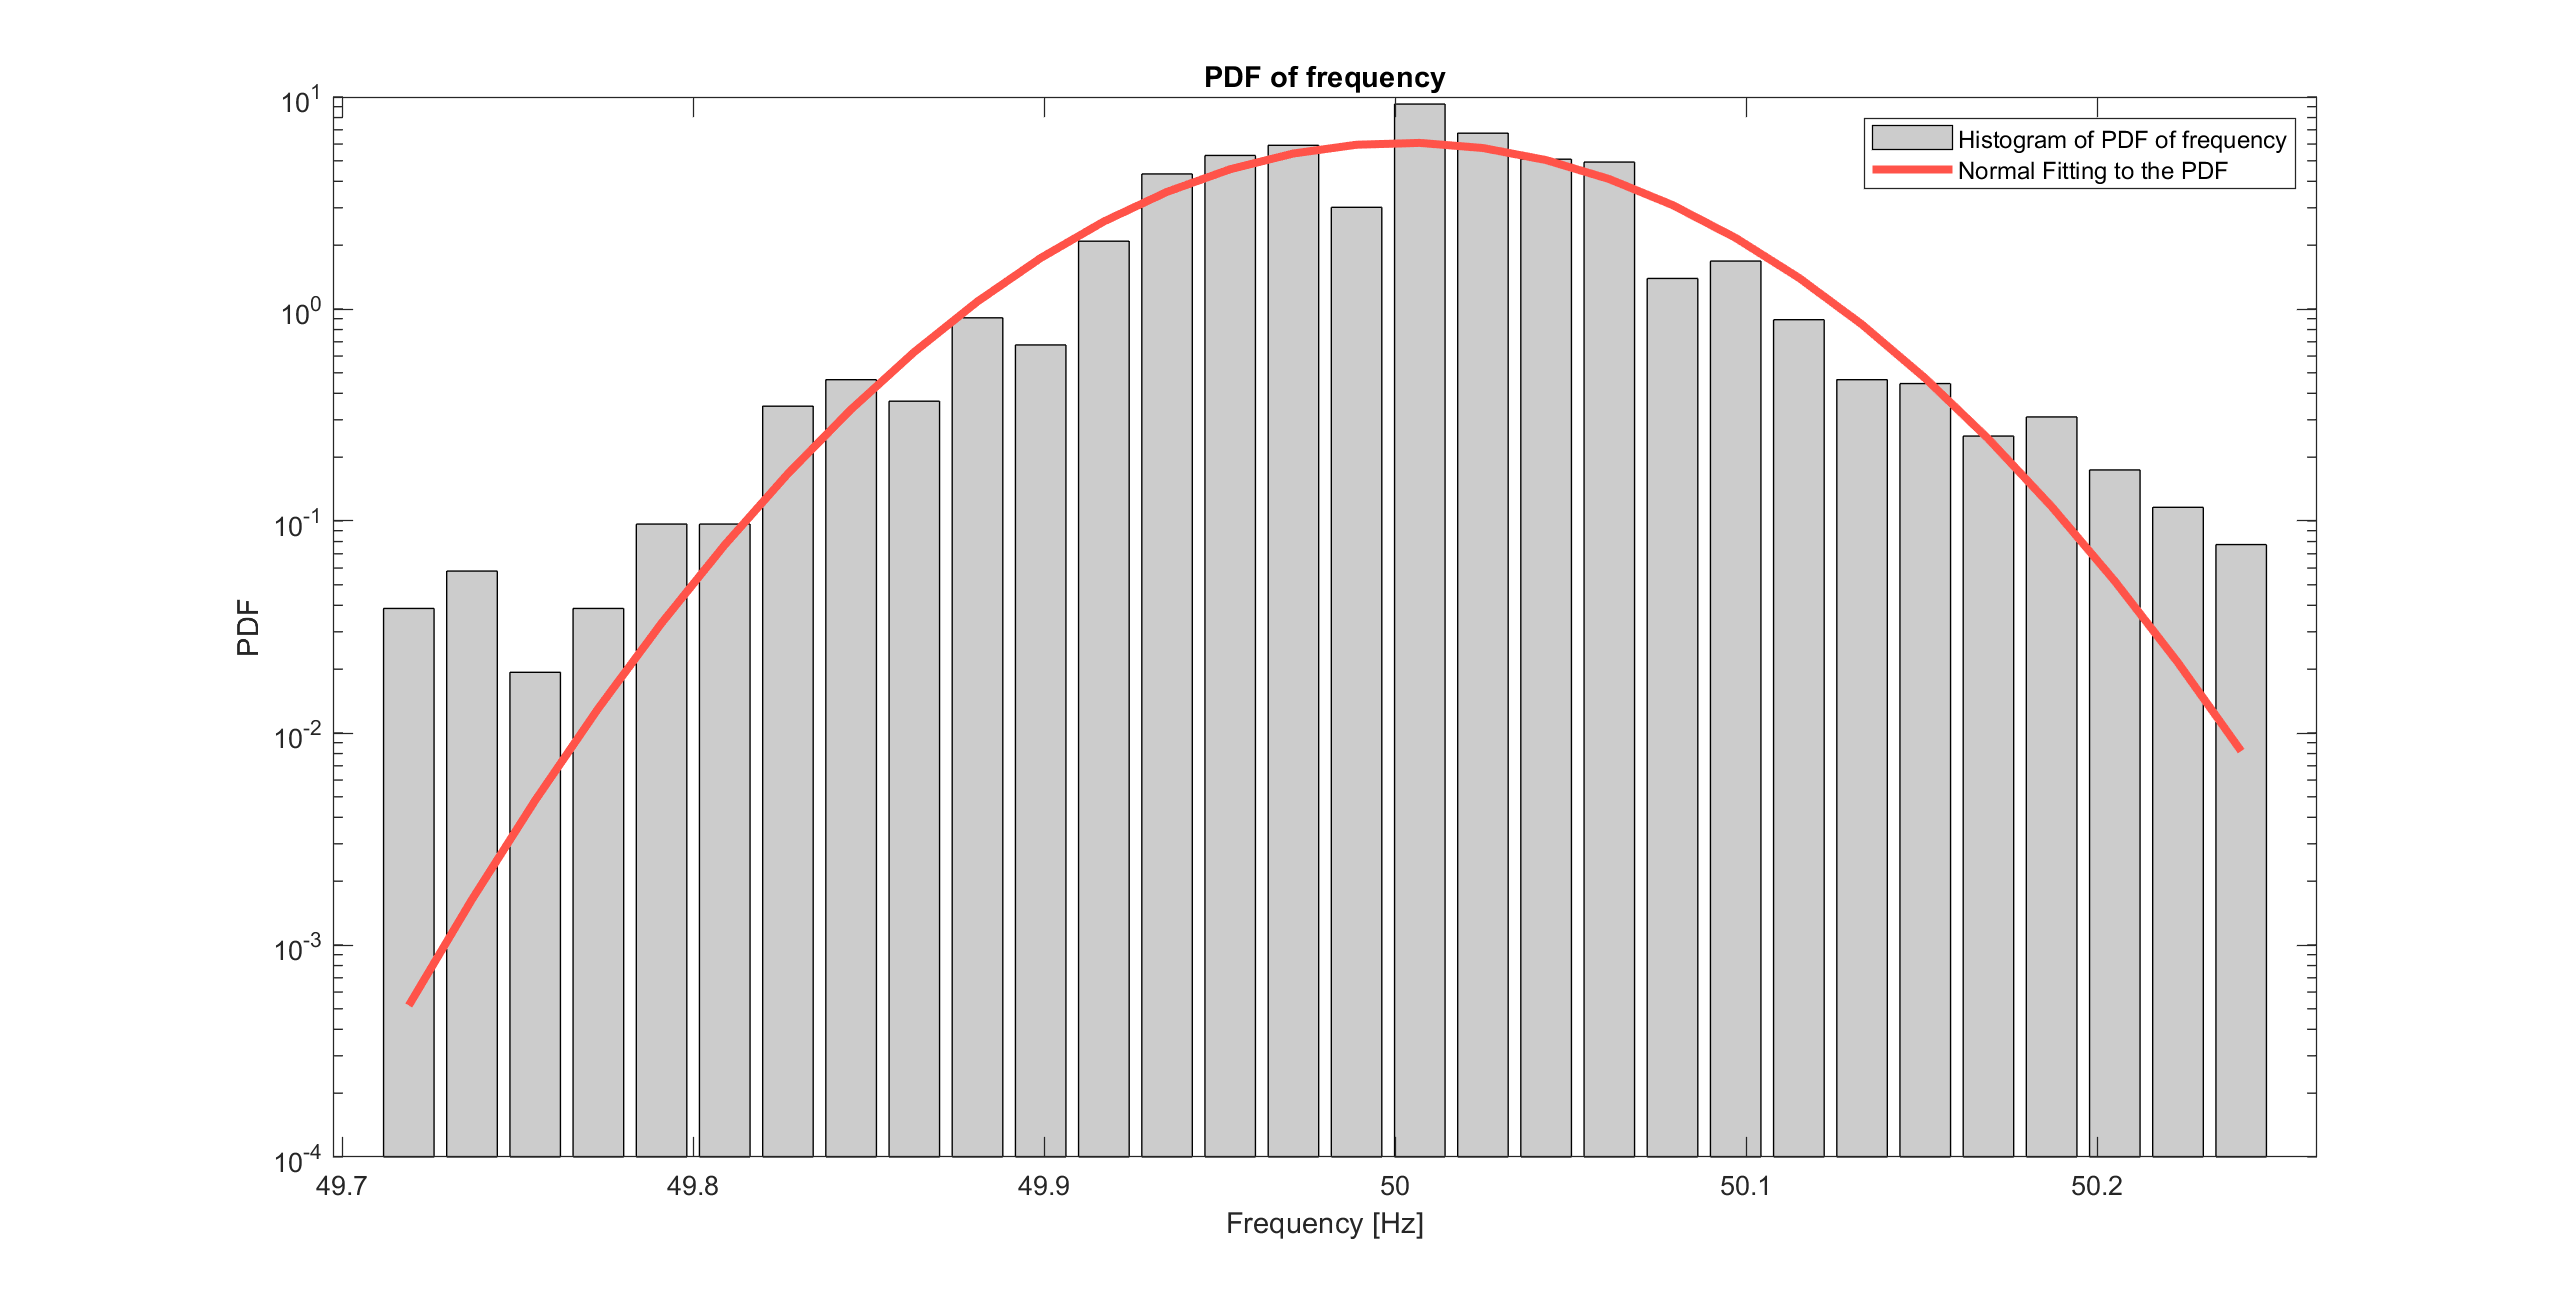
\includegraphics[width=.45\textwidth]{../figures/pdf/nrldc/pdf_frequency_nrldc_06}
	
	\caption{Frequency Probability Density Function Plots for six non-continuous days of the Indian grid (NRLDC). The frequency PDFs show considerable difference among themselves.}
\end{figure}

Similarly, for smaller total sampling durations, the bulk distribution frequency PDF plots are also susceptible to outliers and therefore not ideal for modelling the grid frequency distributions. For example, the available data for the Western Connection Grids and the Texas Grid, both from USA, was small at 3 days and 7 days respectively.

\begin{figure}[!ht]
	\centering
	\begin{subfigure}{\textwidth}
		\centering
		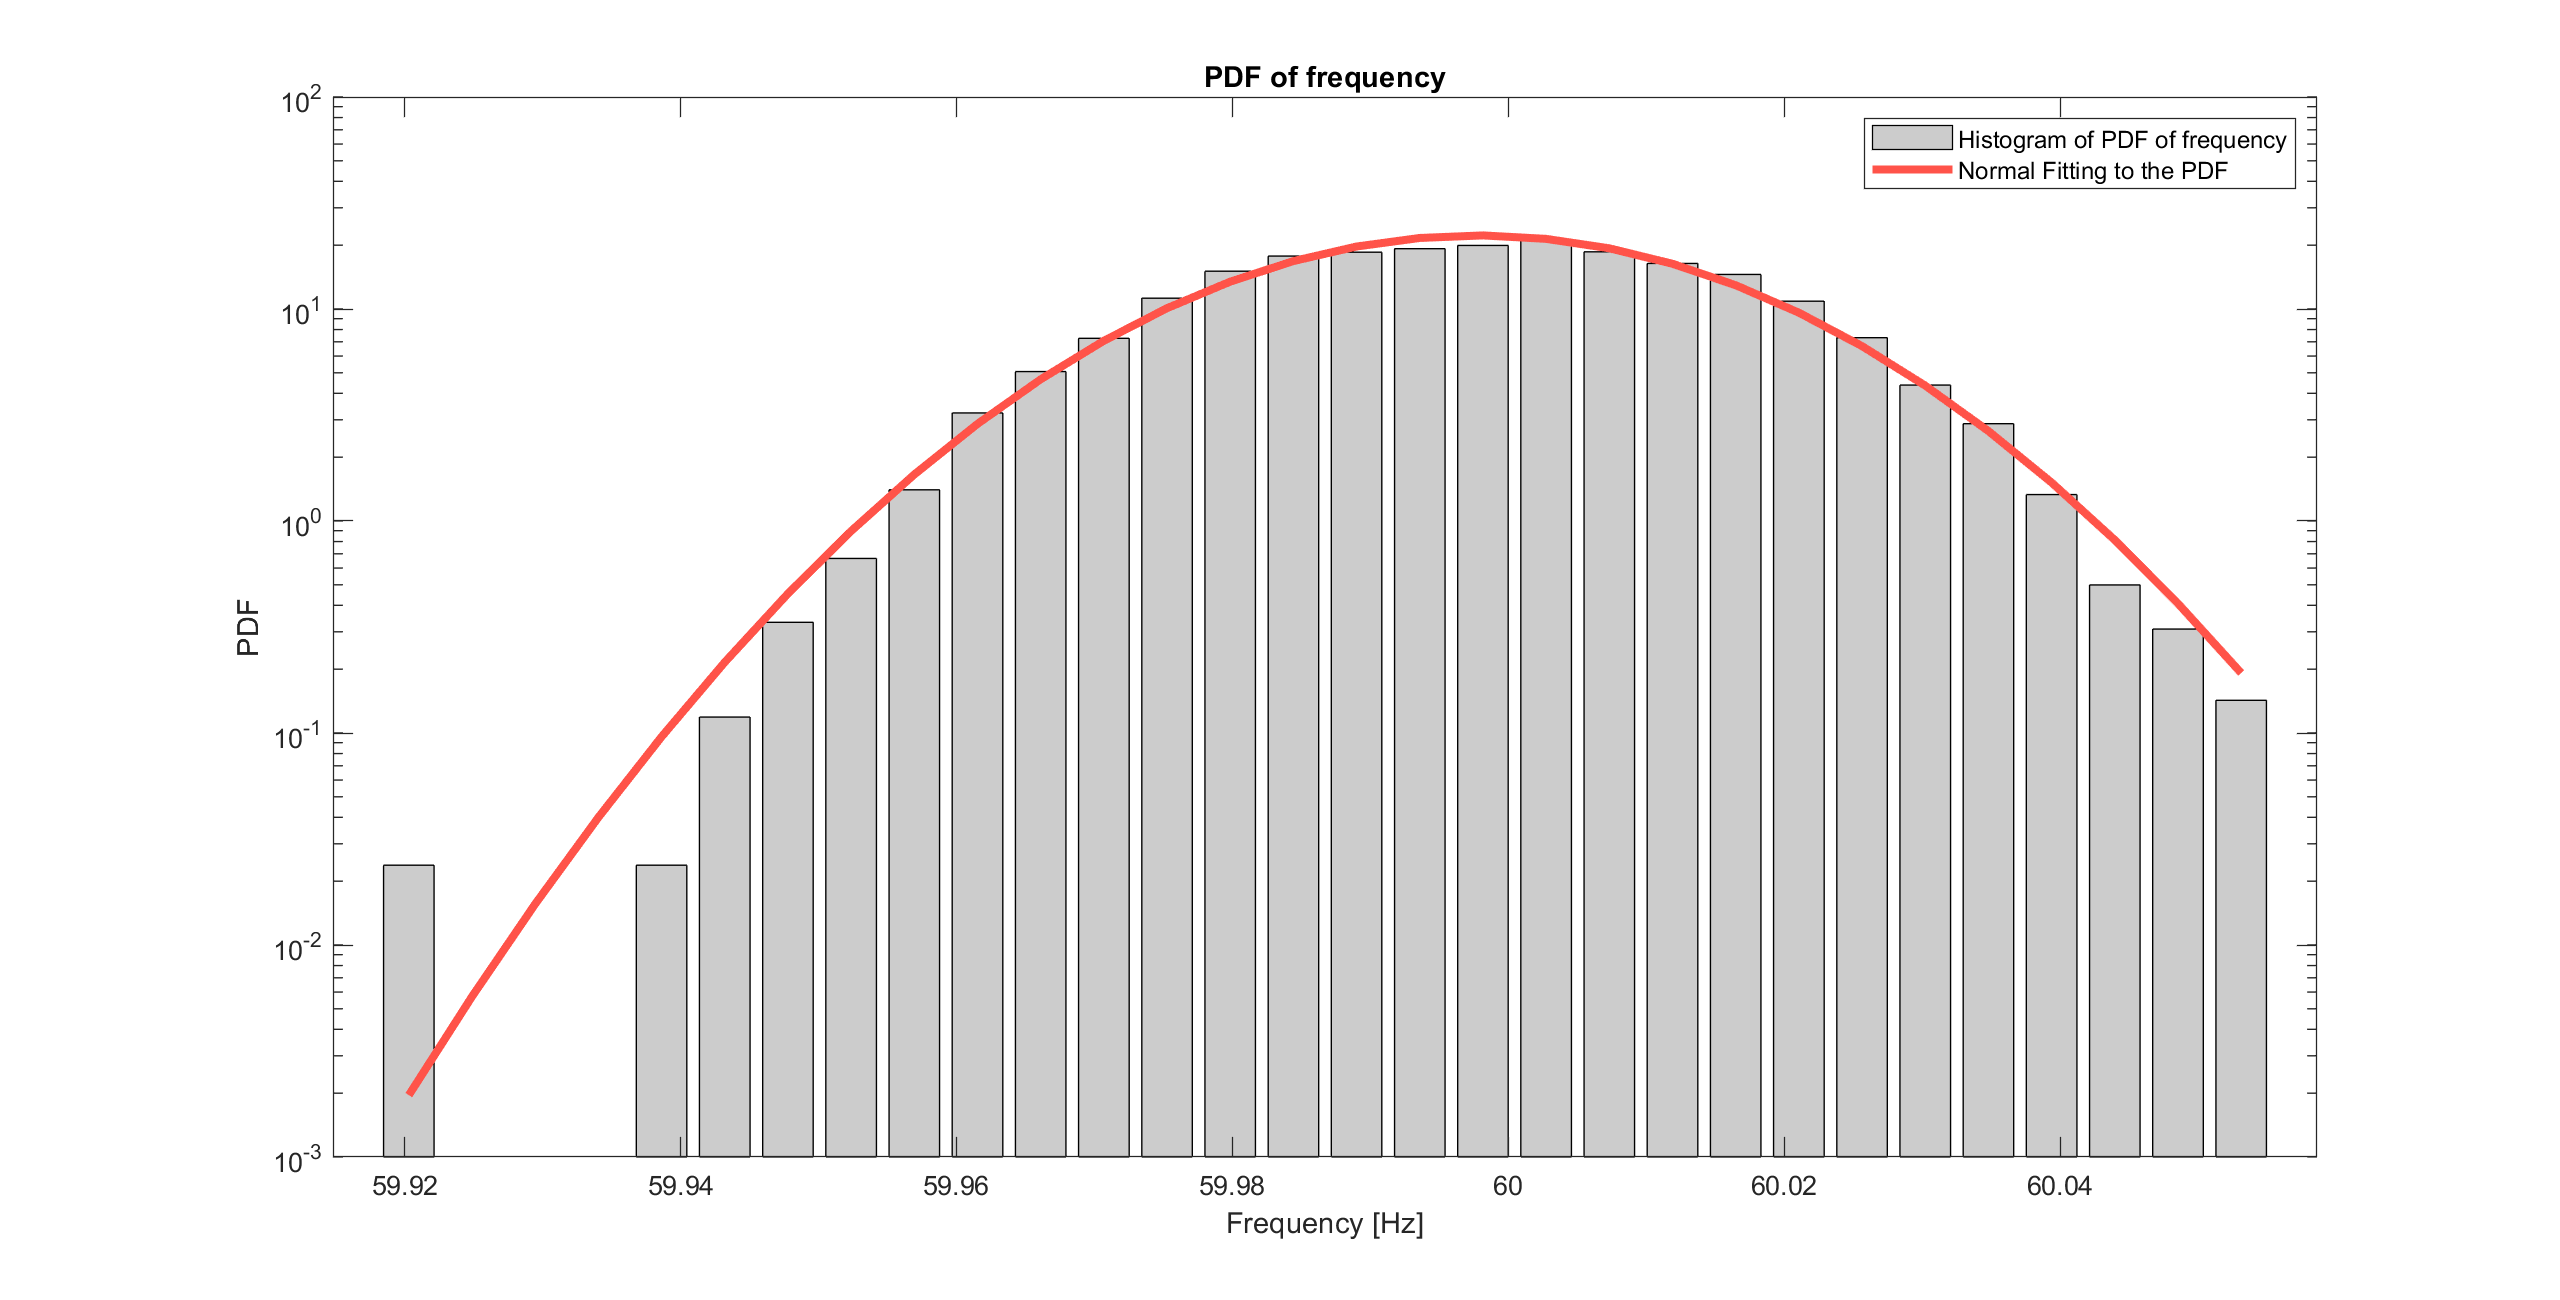
\includegraphics[scale=0.25]{../figures/pdf/pdf_frequency_us_wi_2019_05}
		\caption{Frequency Probability Density Function plot for the Western Interconnection grid in USA for 7 days of May 2019.}
	\end{subfigure}
	
	\begin{subfigure}{\textwidth}
		\centering
		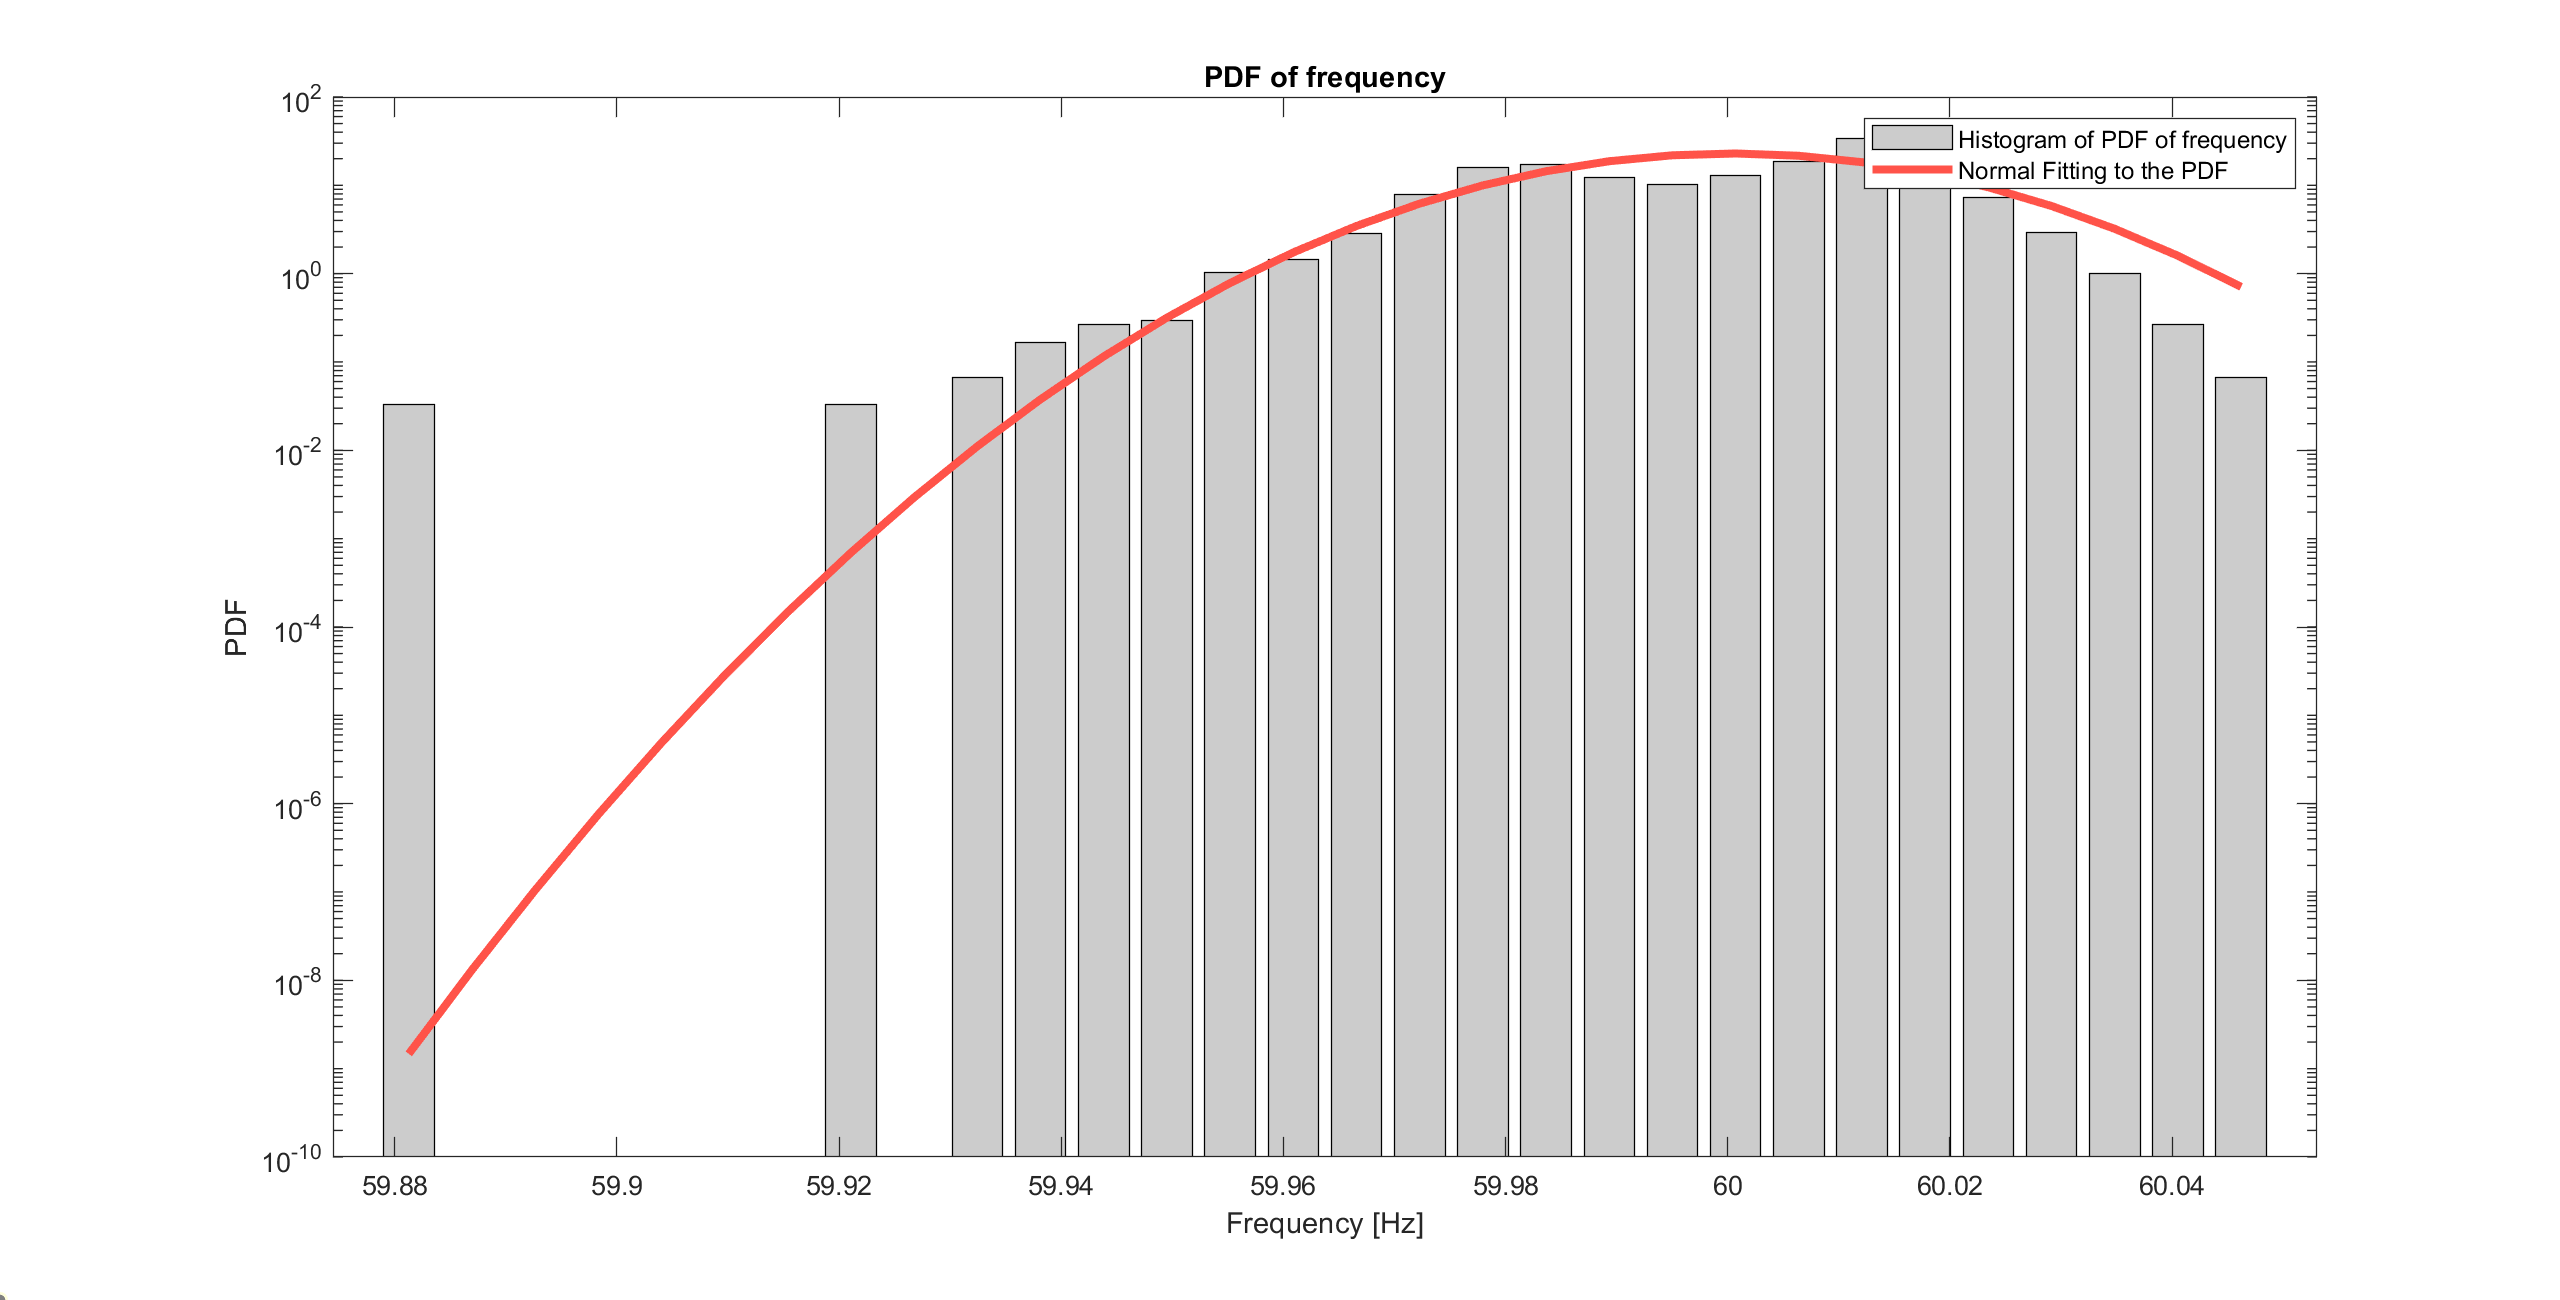
\includegraphics[scale=0.25]{../figures/pdf/pdf_frequency_us_tx_2019_05}
		\caption{Frequency Probability Density Function plot for the Texas Grid for 3 days of May 2019.}
	\end{subfigure}
	\caption{The Texas and Western Interconnection grid frequencies both show outliers in the distribution PDFs, despite not having any faults or major incidences during the sampling period. If the total sampled durations are too low, the frequency distribution PDFs are too susceptible to any major fluctuations, and therefore not reliable models to assume the actual grid frequency distribution PDFs on.}
\end{figure}

Thus a minimum of one month could be considered a sufficient duration to model the bulk characteristics of a grid.